\section{Strato limite su placca piana}\label{c9}
La presente esercitazione si pone come obiettivo la caratterizzazione dello strato limite su una placca piana mediante l'utilizzo dell'anemometria a filo caldo. In particolare, si vuole:
\begin{itemize}
    \item Misurare i profili di velocità per diverse ascisse $x$ con assegnata $U_\infty$;
    \item Caratterizzare la struttura dello strato limite:
    \begin{itemize}
        \item diagrammare i profili di velocità $u=u(x,y)$ e della deviazione standard delle fluttuazioni turbolente longitudinali $u_{rms}(x,y)$;
        \item valutare lo spessore geometrico $\delta(x)$, lo spessore di spostamento $\delta^*(x)$, lo spessore di quantità di moto $\theta(x)$ e il parametro di forma $H(x)$;
        \item verificare la condizione dello strato limite: laminare, transizionale o turbolento;
        \item diagrammare i profili di velocità media e fluttuante nella forma adimensionale: $u/U_\infty = f(y/\delta)$ e $u_{rms}/U_\infty = f(y/\delta)$.
    \end{itemize}
\end{itemize}

\subsection{Descrizione dell'esperimento}
A governare il campo di moto è il numero di Reynolds e in relazione al valore assunto localmente ($Re_{x}=U_\infty\cdot x/\nu$) lo strato limite può essere laminare oppure turbolento.
\begin{figure}[H]
    \centering
    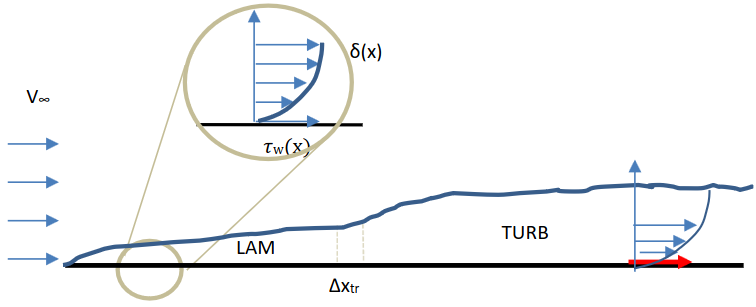
\includegraphics[width=.8\textwidth]{images/9/slimage.png}
    \caption{Rappresentazione dello strato limite}
\end{figure}

\noindent Se il numero di Reynolds locale supera il numero di Reynolds critico $Re_{cr}$ allora si ha strato limite turbolento, altrimenti si ha strato limite laminare. Dal numero di Reynolds critico si può quindi individuare la coordinata $x_{tr}$ di transizione:
\begin{equation*}
    Re_{cr}=\frac{U_\infty \cdot x_{tr}}{\nu}=5\cdot10^5
\end{equation*}
Per una placca piana posta ad incidenza nulla in un flusso senza turbolenza il numero di Reynolds critico vale $Re_{cr}\approx5\cdot10^5$. Se invece è presente turbolenza la transizione dello strato limite è anticipata, pertanto il numero di Reynolds critico risulta inferiore.\\\\
Per una data lunghezza $L$ della placca e conoscendo il valore della velocità della corrente a monte è possibile definire il numero di Reynolds globale della placca:
\begin{equation*}
    Re_L = \frac{U_\infty \cdot L}{\nu}
\end{equation*}
Nel caso di strato limite laminare la soluzione delle equazioni porta alla soluzione di Blasius, che definisce il profilo di velocità adimensionale sotto forma di tabella:
\begin{equation*}
    \eta(x,y) \approx \frac{y}{\delta(x)} = y\sqrt{\frac{U_\infty}{\nu x}} \qquad f^\prime = \frac{u}{V_\infty}
\end{equation*}
Per lo strato limite laminare sono valide le seguenti relazioni empiriche:
\begin{equation*}
    \delta(x) = \frac{5x}{\sqrt{Re_x}} \qquad \delta^*(x) = \frac{1.73x}{\sqrt{Re_x}} \qquad \theta(x) = \frac{0.664x}{\sqrt{Re_x}} \qquad H(x) = \frac{\delta^*}{\theta}
\end{equation*}
\begin{equation*}
    \tau_w(x) = 0.332 \sqrt{\frac{\rho \mu U_\infty^3}x} \qquad c_f(x) = \frac{0.664}{\sqrt{Re_x}} \qquad c_D = \frac{1.328}{\sqrt{Re_L}}
\end{equation*}
Nel caso di strato limite turbolento è presente una struttura multi-strato costituita principalmente da due regioni: inner layer ed outer layer.\\\\
L'inner layer, che copre una frazione pari al 10\%-20\% dello spessore dello strato limite $\delta$, a sua volta è costituito da tre substrati: il sottostrato viscoso, il buffer layer e la regione logaritmica.
\begin{figure}[H]
    \centering
    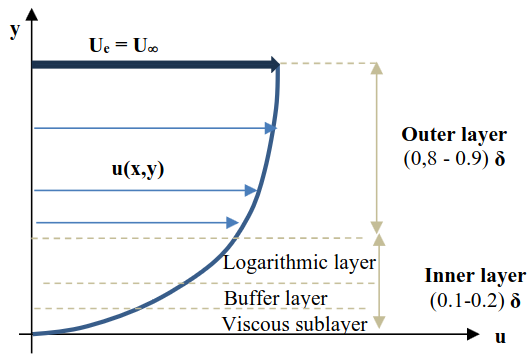
\includegraphics[width=.55\textwidth]{images/9/sltimage.png}
    \caption{Rappresentazione del profilo di velocità in uno strato limite turbolento}
\end{figure}

\noindent Per lo strato limite turbolento si definisce la velocità di attrito:
\begin{equation*}
    u_\tau = \sqrt{\frac{\tau_w}{\rho}}
\end{equation*}
E la lunghezza di attrito:
\begin{equation*}
    l_\tau = \frac{\nu}{u_\tau}
\end{equation*}
Se la velocità $u(y)$ si adimensionalizza rispetto alla velocità di attrito $u_\tau$ e la distanza da parete $y$ rispetto alla lunghezza di attrito $l_\tau$, la distribuzione di velocità si può presentare nella forma adimensionale più appropriata per lo studio dello strato limite turbolento, ovvero si esprime $u^+ = f(y^+)$. Le nuove variabili sono quindi definite come:
\begin{equation*}
    y^+ = \frac{y}{l_\tau} \qquad u^+ = \frac{u}{u_\tau}
\end{equation*}
Trattandosi di strato limite turbolento la velocità è da intendersi come velocità media nel tempo. Per il sottostrato viscoso e la regione logaritmica dell'inner layer sono definite opportune leggi di distribuzione della velocità $u^+=f(y^+)$:
\begin{itemize}
    \item Sottostrato viscoso: $0 \le y^+ \le 5$
    \begin{equation*}
        u^+ = y^+
    \end{equation*}
    \item Regione logaritmica: $30 \le y^+ \le 500$
    \begin{equation*}
        u^+ = \frac{1}{k}log(y^+) + B
    \end{equation*}
    con $k = 0.41$ (costante di Von Karman) e $B = 5.2$ (costante di Coles).
\end{itemize}

\noindent L'estremo superiore (500) della regione logaritmica in generale dipende dal numero di Reynolds e dal gradiente di pressione.
\begin{figure}[H]
    \centering
    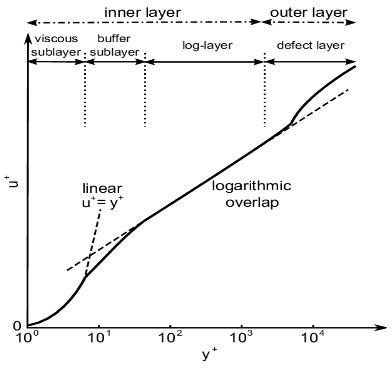
\includegraphics[width=.55\textwidth]{images/9/slinnerimage.png}
    \caption{Rappresentazione del profilo di velocità nell'inner layer}
\end{figure}

\noindent Per lo strato limite turbolento incomprimibile valgono le seguenti relazioni empiriche:\\\\
\textbf{Bassa turbolenza ($5\cdot10^5<Re<10^7$)}
\begin{equation*}
    \delta(x) = \frac{0.370x}{Re_x^{1/5}} \qquad q^*(x) = \frac{0.04625 x}{Re_x^{1/5}} \qquad \theta(x) = \frac{0.0360 x}{Re_x^{1/5}} \qquad H=\frac{\delta^*(x)}{\theta(x)}
\end{equation*}
\begin{equation*}
    \tau_w(x) = \frac{0.0288 \rho U^2}{Re_x^{1/5}} \qquad c_f = \frac{0.0576}{Re_x^{1/5}} \qquad \overline \tau_w = \frac{0.036\rho U^2}{Re_L^{1/5}} \qquad c_D = \frac{0.074}{Re_L^{1/5}}
\end{equation*}
\textbf{Alta turbolenza ($Re>10^7$)}
\begin{equation*}
    \delta(x) = \frac{0.232x}{Re_x^{1/7}} \qquad q^*(x) = \frac{0.0193 x}{Re_x^{1/5}} \qquad \theta(x) = \frac{0.0164 x}{Re_x^{1/5}} \qquad H=\frac{\delta^*(x)}{\theta(x)}
\end{equation*}
\begin{equation*}
    \tau_w(x) = \frac{0.0115 \rho U^2}{Re_x^{1/7}} \qquad c_f = \frac{0.0230}{Re_x^{1/7}} \qquad \overline \tau_w = \frac{0.0134\rho U^2}{Re_L^{1/7}} \qquad c_D = \frac{0.0295}{Re_L^{1/7}}
\end{equation*}

\subsection{Catena di misura}
La galleria del vento è del tipo a circuito aperto-aspirato con camera di prova circolare e chiusa.\\\\
All'interno della camera di prova è posta una placca piana, a contatto con le pareti della galleria in modo da rendere il flusso il più bidimensionale possibile.\\\\
La sonda a filo caldo è posizionata in prossimità della placca piana mediante un movimentatore verticale elettromeccanico passo-passo, in grado di spostare verticalmente la sonda di un millimetro per ogni 200 passi.\\\\
Il sistema sonda-movimentatore passo-passo, è posizionato lungo la mezzeria della galleria placca piana, ad una distanza $x$ misurata approssimativamente dal bordo di attacco.\\\\
Nella catena di misura è inoltre presente un tubo di Pitot necessario per regolare la velocità del flusso nella galleria del vento ed un sistema di acquisizione dati.
\begin{figure}[H]
    \centering
    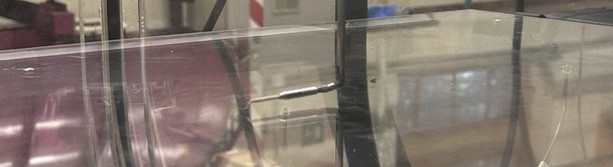
\includegraphics[width=.8\textwidth]{images/9/sonda.jpg}
    \caption{Sonda a filo caldo posizionata in prossimità della placca piana}
\end{figure}

\begin{figure}[H]
    \centering
    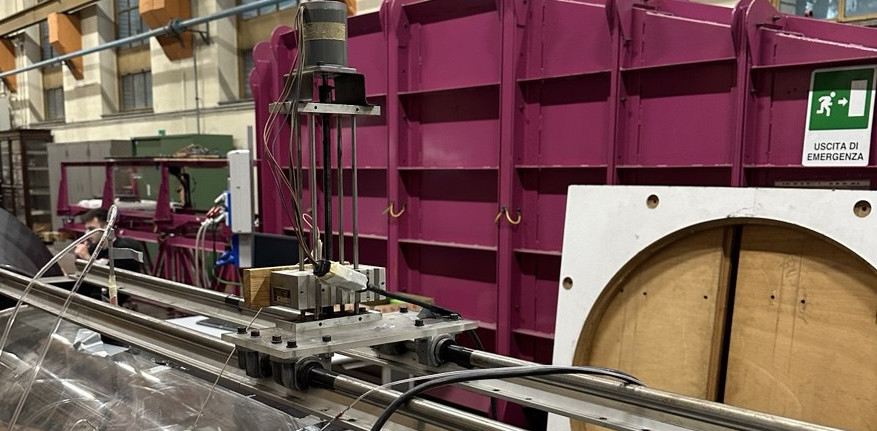
\includegraphics[width=\textwidth]{images/9/passopasso.jpg}
    \caption{Motore passo-passo e slitta per il posizionamento della sonda}
\end{figure}
\begin{figure}[H]
    \centering
    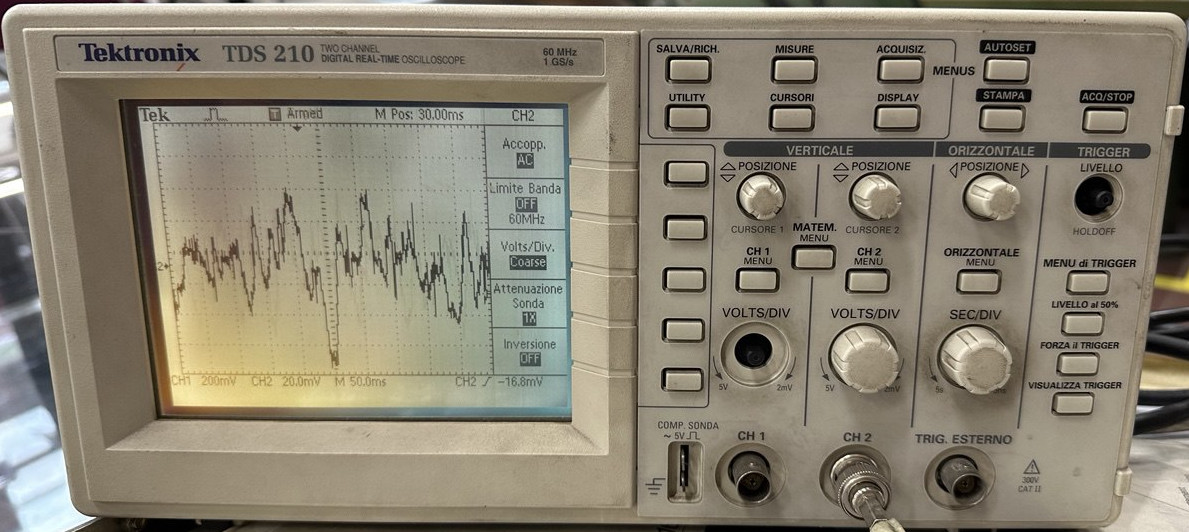
\includegraphics[width=\textwidth]{images/9/anem1.jpg}
    \caption{Anemometro}
\end{figure}

\newpage
\subsection{Procedura sperimentale}
Come prima operazione si calcola la densità e la viscosità dinamica, a partire dalla pressione e dalla temperatura ambiente, utilizzando la legge dei gas perfetti e la legge di Sutherland:
\begin{equation*}
    \rho = \frac{p_{amb}}{RT_{amb}} \qquad \mu = 1.46\cdot10^{-6} \frac{T_{amb}^{3/2}}{T_{amb}+110}
\end{equation*}
Ogni esperimento viene effettuato ad una determinata distanza $x$, misurata in modo approssimativo dal bordo d'attacco della placca piana. La galleria del vento è inoltre impostata ad una velocità costante $U_\infty$, misurata dal tubo di Pitot. Si eseguono misure su due configurazioni $(x,U_\infty)$ per ognuna delle quattro squadre, per un totale di otto configurazioni:\\
Squadra 1: ($x = 0.55$ m, $U_\infty= 8.7$ m/s), ($x = 0.9$ m, $U_\infty= 8.7$ m/s)\\
Squadra 2: ($x = 0.50$ m, $U_\infty= 10.9$ m/s), ($x = 0.9$ m, $U_\infty= 10.9$ m/s)\\
Squadra 3: ($x = 0.9$ m, $U_\infty= 11$ m/s), ($x = 0.9$ m, $U_\infty= 3.6$ m/s)\\
Squadra 4: ($x = 0.7$ m, $U_\infty= 3.1$ m/s), ($x = 0.7$ m, $U_\infty= 10.8$ m/s)\\\\
Prima di azionare la galleria del vento, è bene misurare la tensione di offset $E_0$ della sonda a filo caldo, in modo da poter ricavare la costante $A$ della legge di King per ognuna delle configurazioni:
\begin{equation*}
    E^2 = A + BU^n \qquad A = E_0^2
\end{equation*}
Come costanti $B$ ed $n$ si utilizzano quelle ricavate durante l'attivita precedente.\\\\
La prima posizione della sonda è approssimativamente a mezzo millimetro di distanza $y$ dalla placca piana. In questa posizione si acquisiscono i dati di tensione in uscita dall'anemometro ad una determinata frequenza di campionamento $f_s=200$ Hz per un periodo $T=30$ s.\\\\
La sonda non può avvicinarsi troppo alla placca, perché in caso di contatto, questa potrebbe rompersi. Inoltre, poiché il supporto che tiene la sonda non è infinitamente rigido, il flusso d'aria della galleria ne induce delle vibrazioni, che fanno oscillare la sonda a filo caldo. Se la sonda è troppo vicina alla placca, le oscillazioni possono indurre un contatto e quindi portare al danneggiamento della sonda.\\\\
Una volta acquisiti i primi dati, mediante il sistema di azionamento del motore passo-passo, si aumenta con precisione la distanza della sonda a filo caldo dalla placca piana $y$ e si acquisiscono nuovamente i dati.\\\\
Per ogni configurazione si ottengono quindi $N = f_s\cdot T$ dati campionati ad ogni distanza $y$ considerata.\\\\
Infine, per eseguire un'analisi in frequenza, si esegue una misura ad un'elevata frequenza di campionamento ($f_s=30$ kHz, per la quarta squadra $f_s=20$ kHz) per un periodo di un minuto (55 secondi per la squadra 4).

\subsection{Analisi dati}
L'analisi dati per la presente attività è condotta con l'ausilio di un codice Python, riportato in appendice \ref{b9}.\\\\
Ad ogni valore di tensione in uscita dall'anemometro rilevato, si associa un valore di velocità mediante l'utilizzo della legge di King:
\begin{equation*}
    U_i = \left( \frac{E_i^2-A}B \right)^{1/n}
\end{equation*}
Per ogni stazione di acquisizione, si calcola il valore medio $u(y)$ e la deviazione standard $u_{rms}(y)$ della velocità:
\begin{equation*}
    u(y) = \frac{1}{N}\sum_{i=1}^{N} U_i \qquad u_{rms}(y) = \sqrt{\frac{1}{N}\sum_{i=1}^{N}{\left(U_i - u(y)\right)^2}}
\end{equation*}
A questo punto è già possibile tracciare dei diagrammi dimensionali dei profili di velocità e di deviazione standard:
\begin{figure}[H]
    \centering
    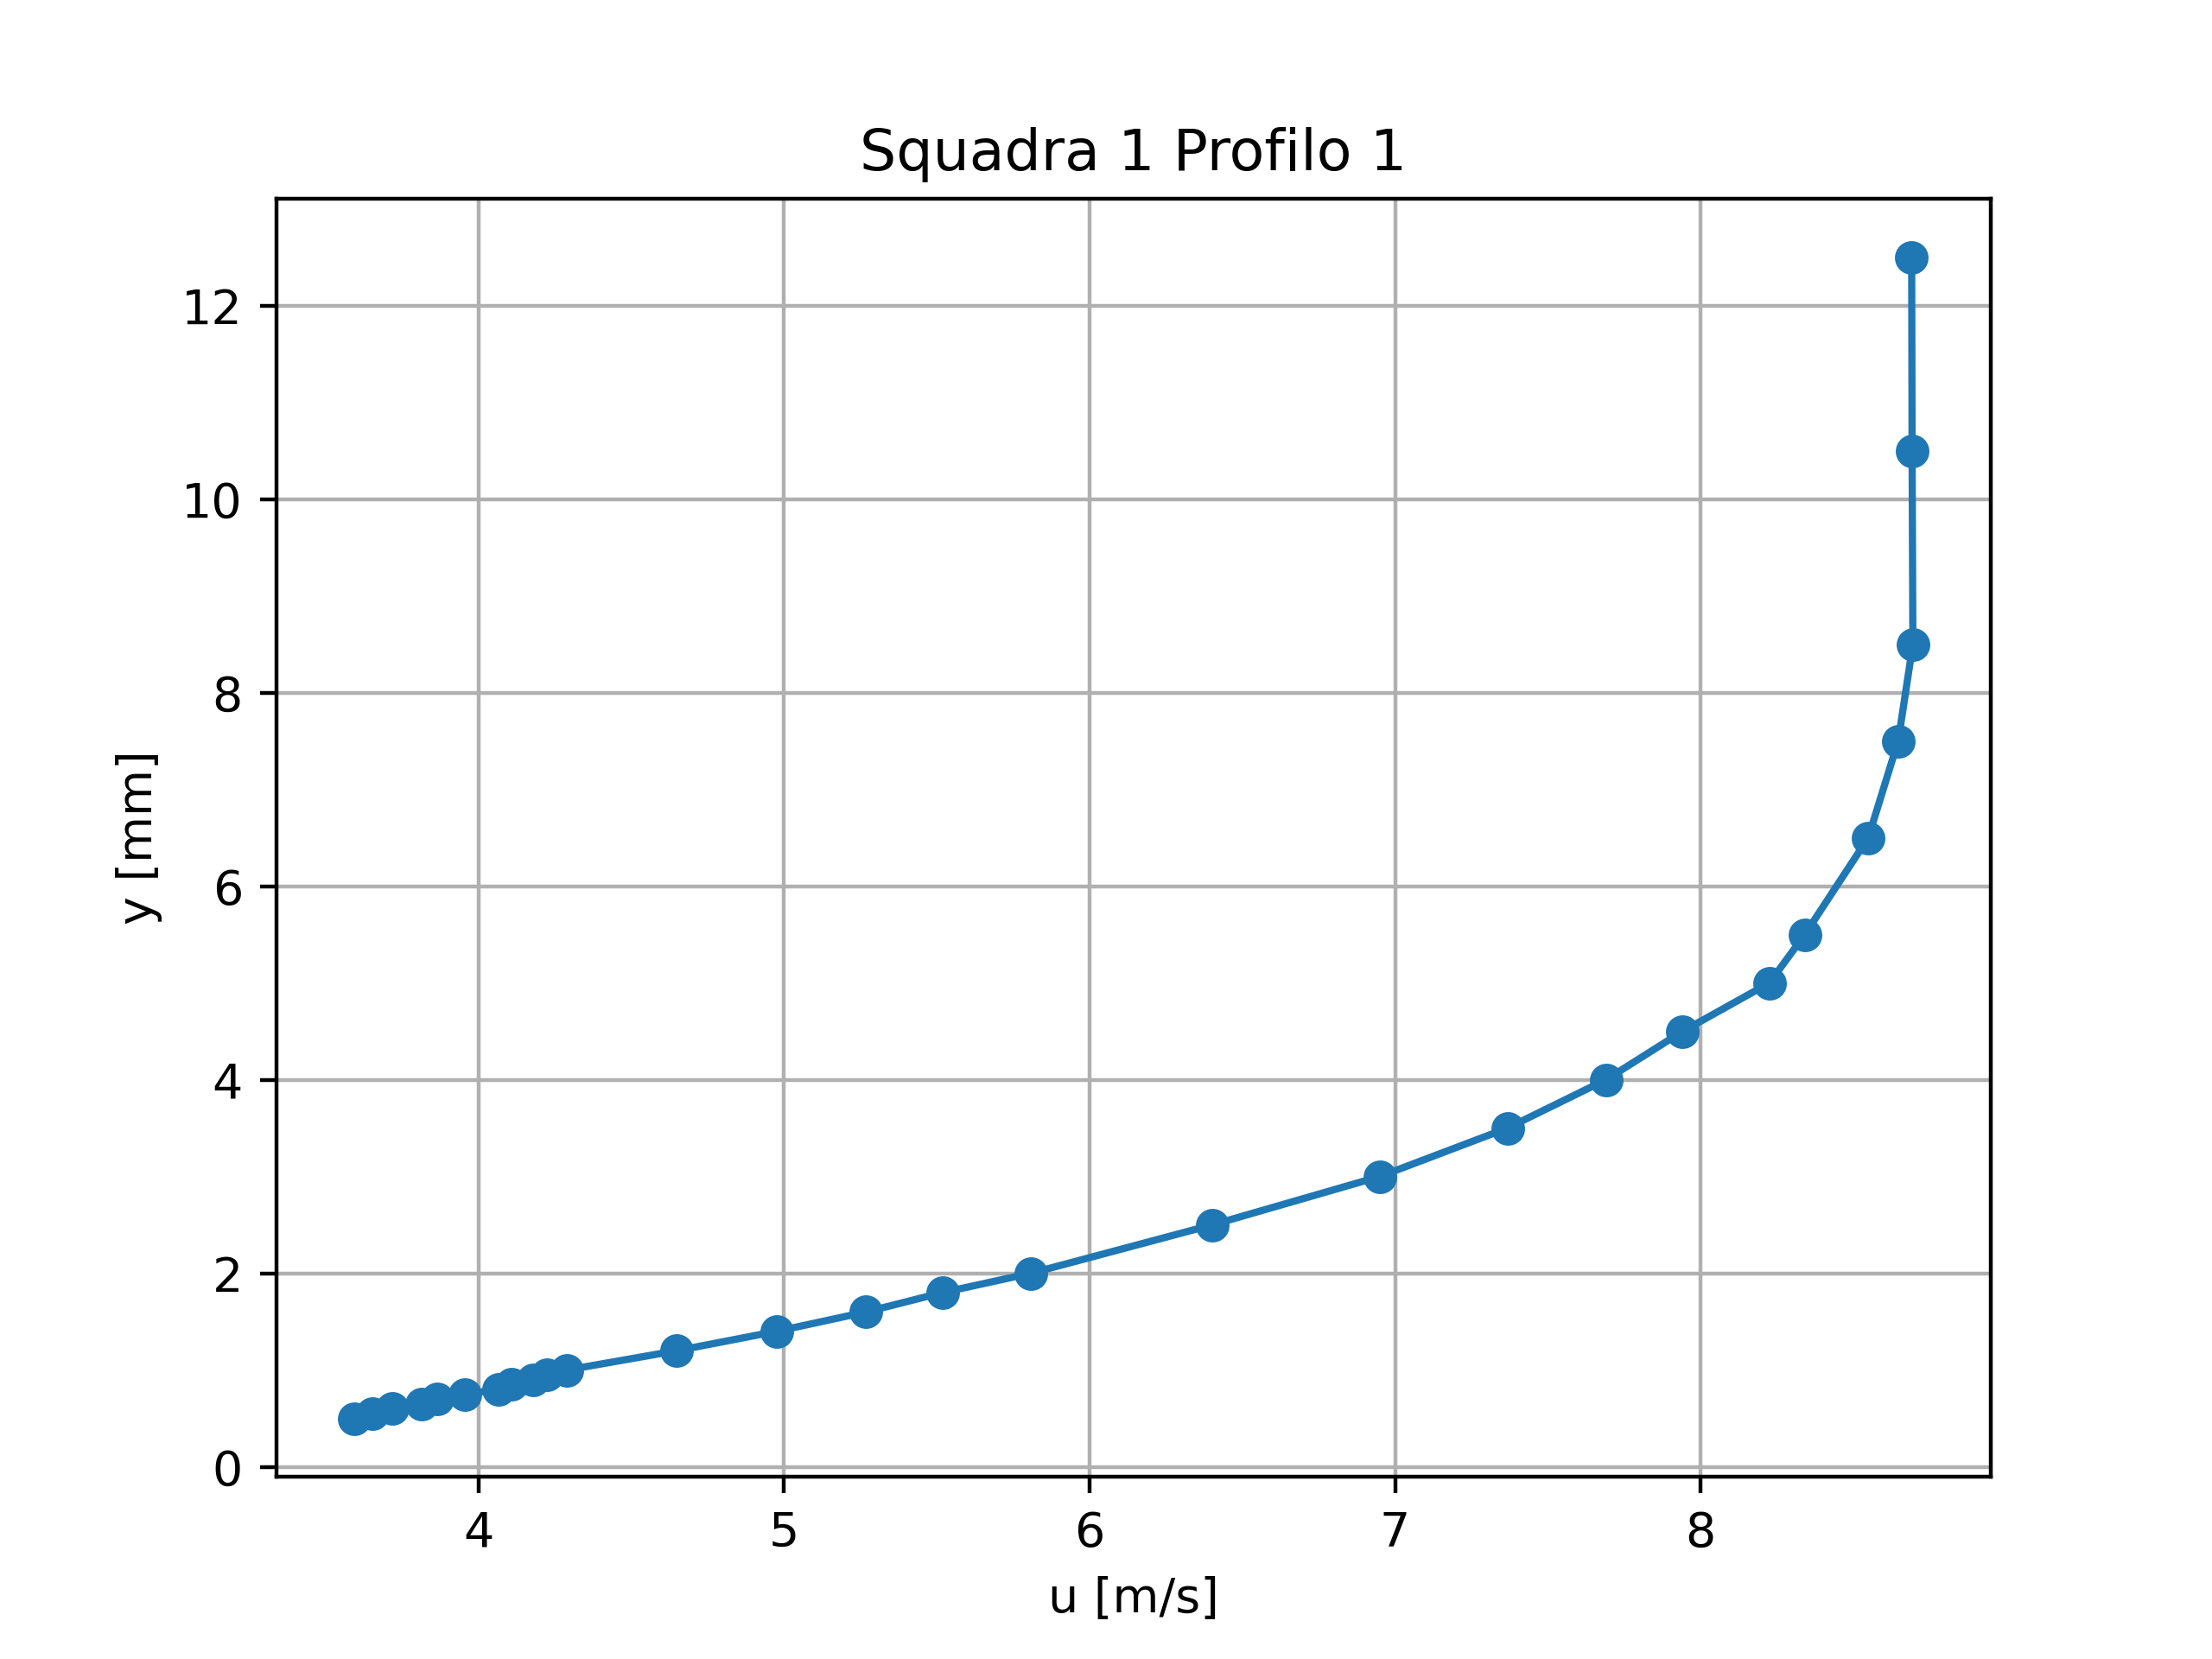
\includegraphics[width=.49\textwidth]{images/9/sq1p1.png}
    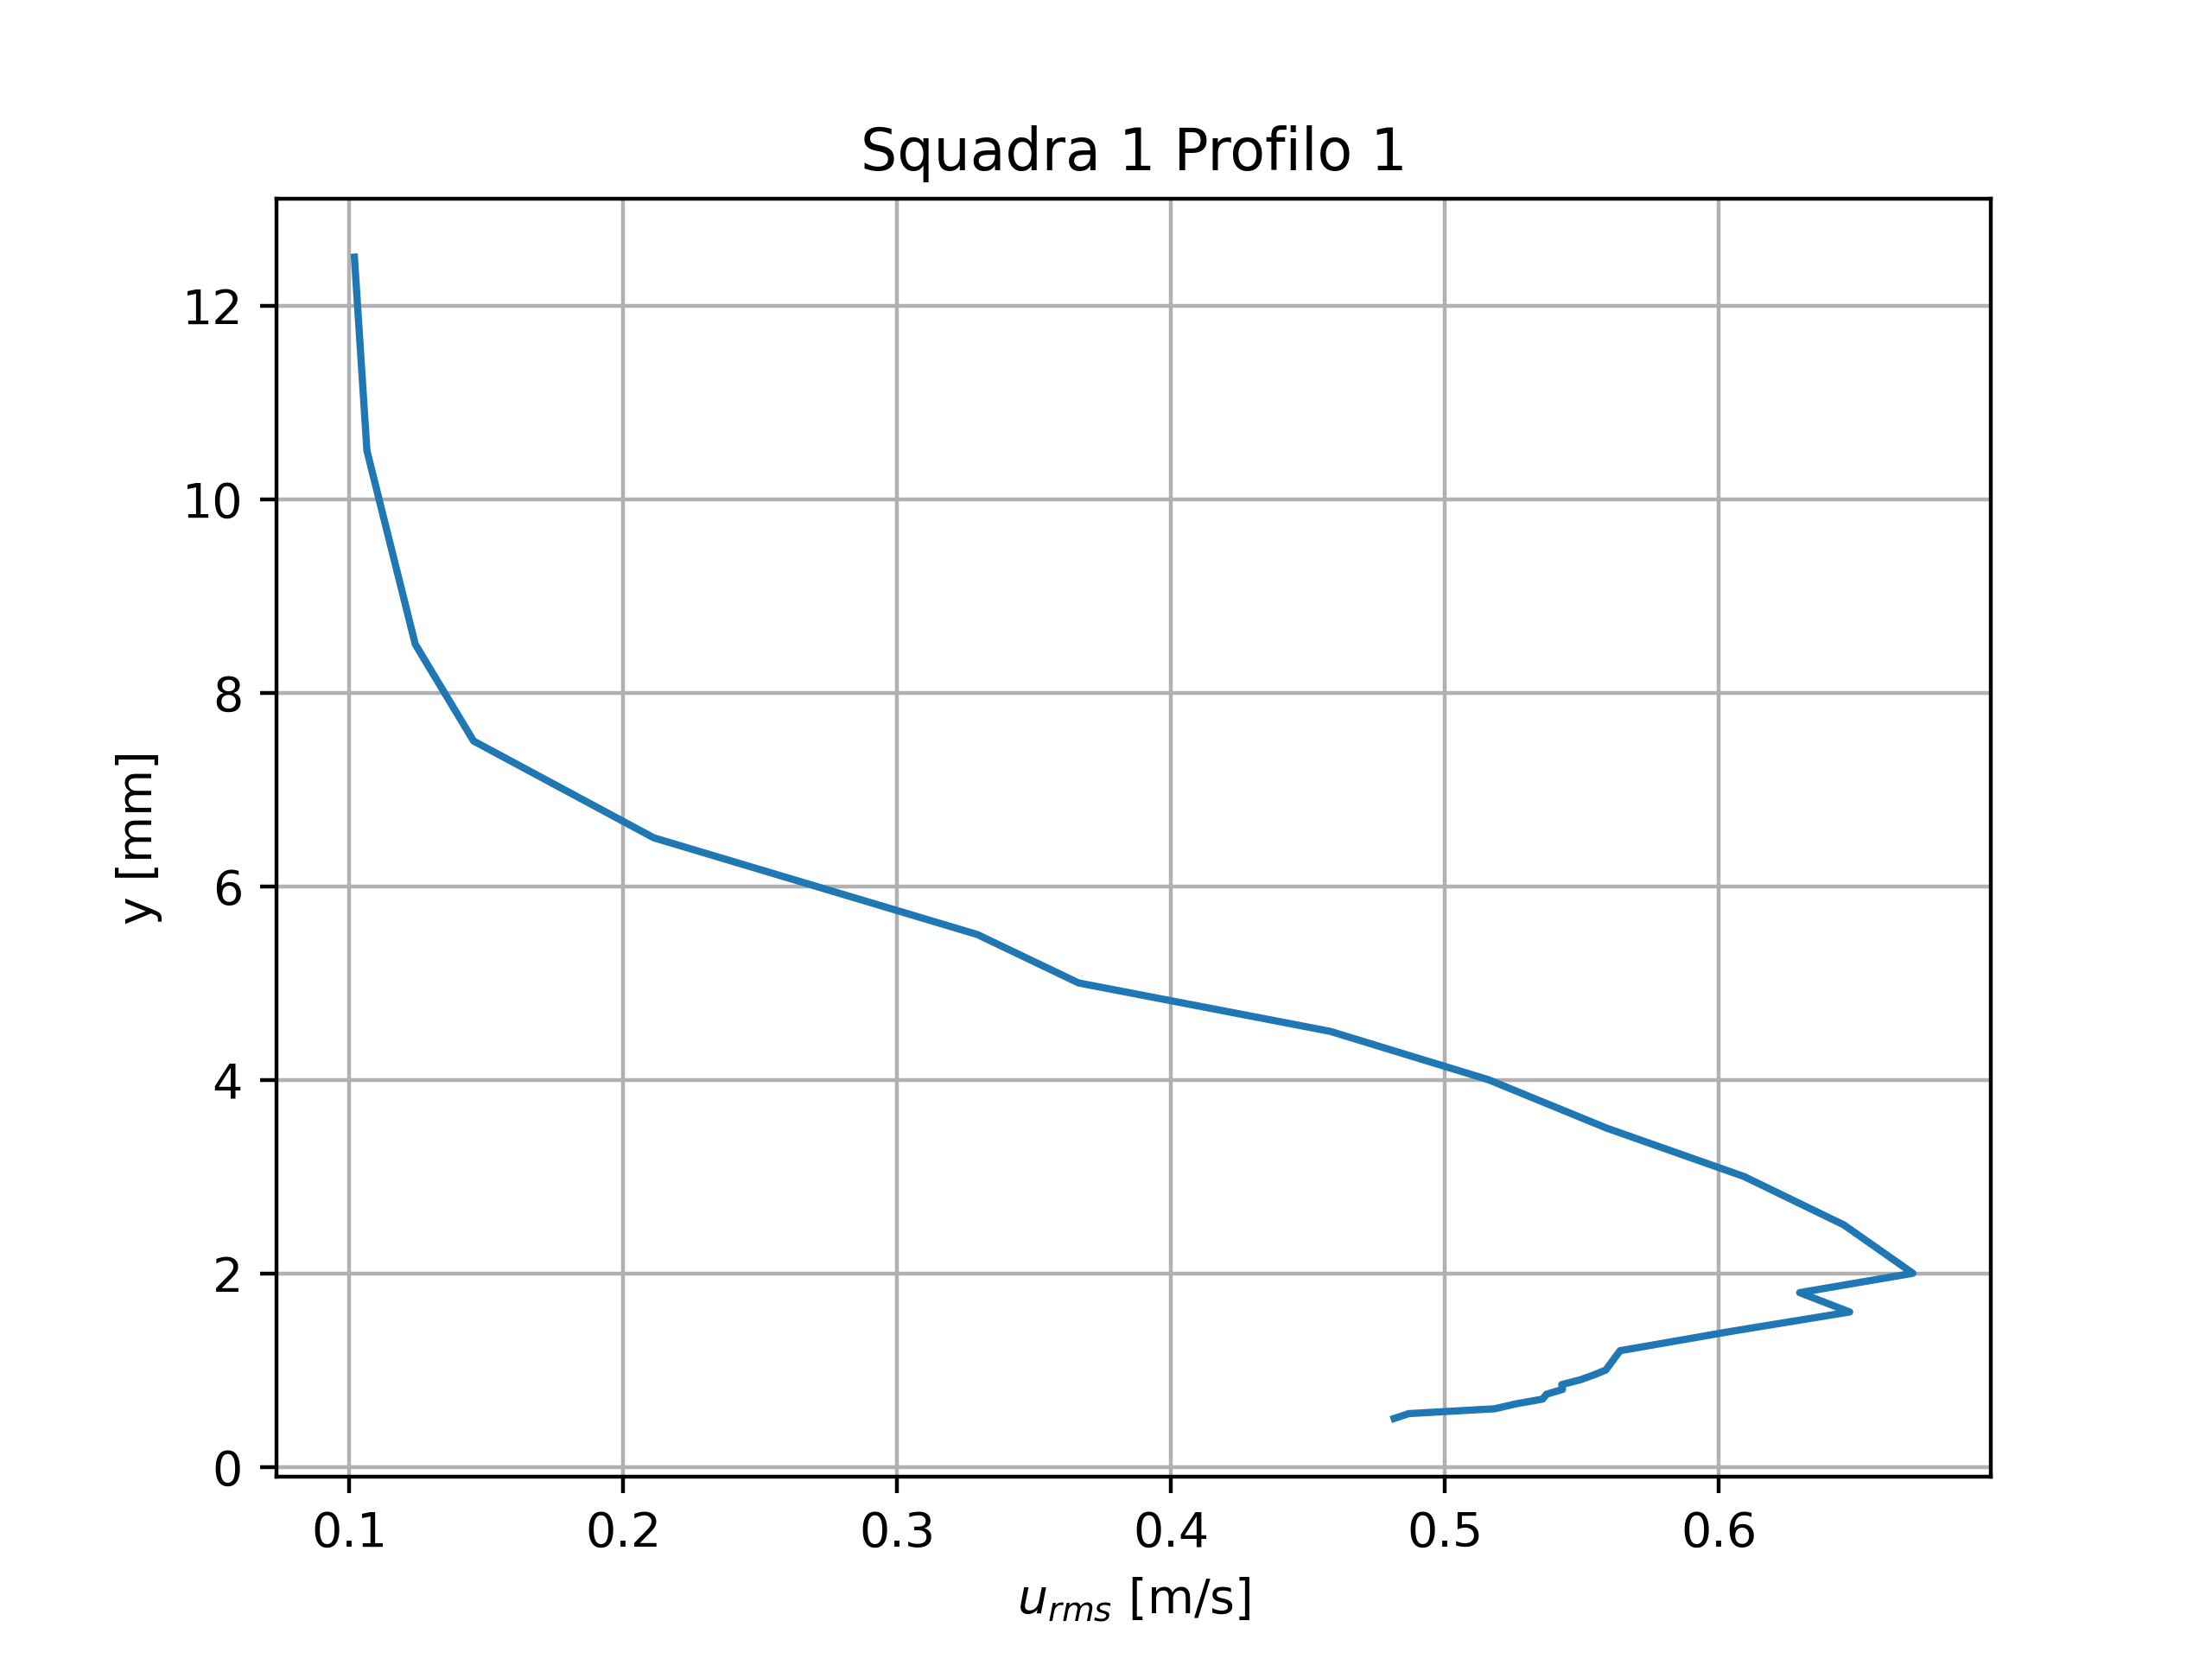
\includegraphics[width=.49\textwidth]{images/9/sq1p1rms.png}
    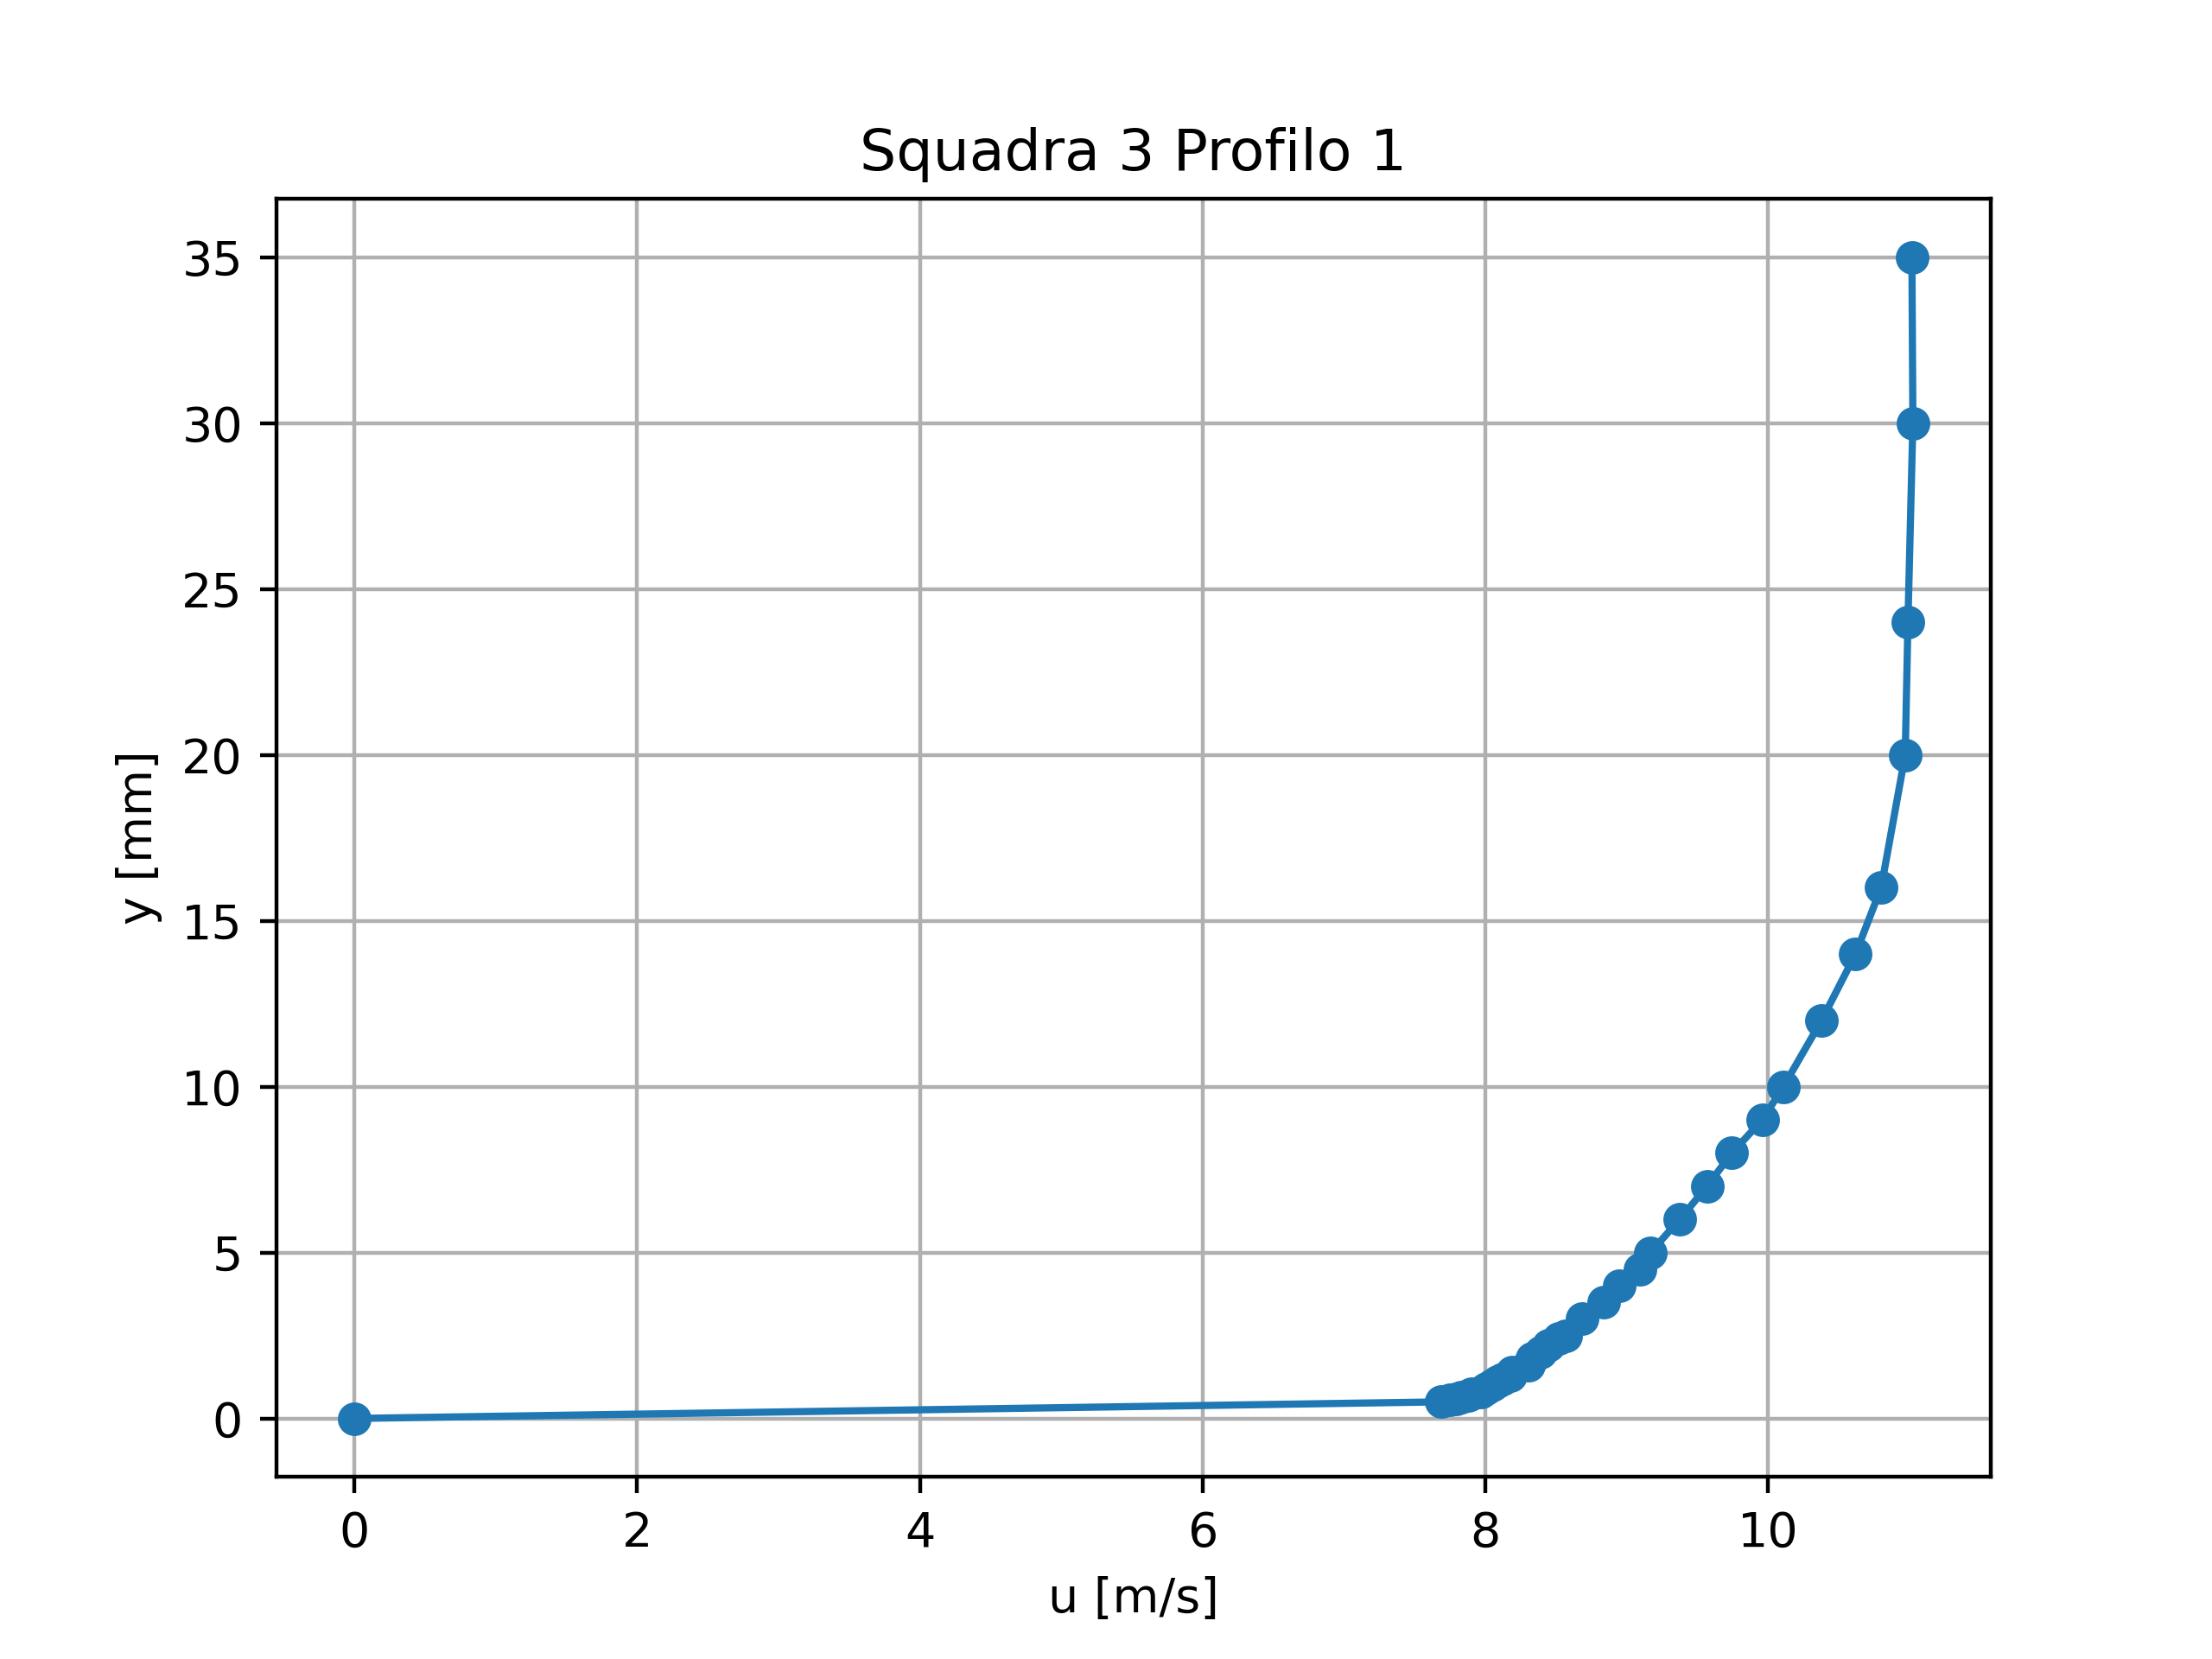
\includegraphics[width=.49\textwidth]{images/9/sq3p1.png}
    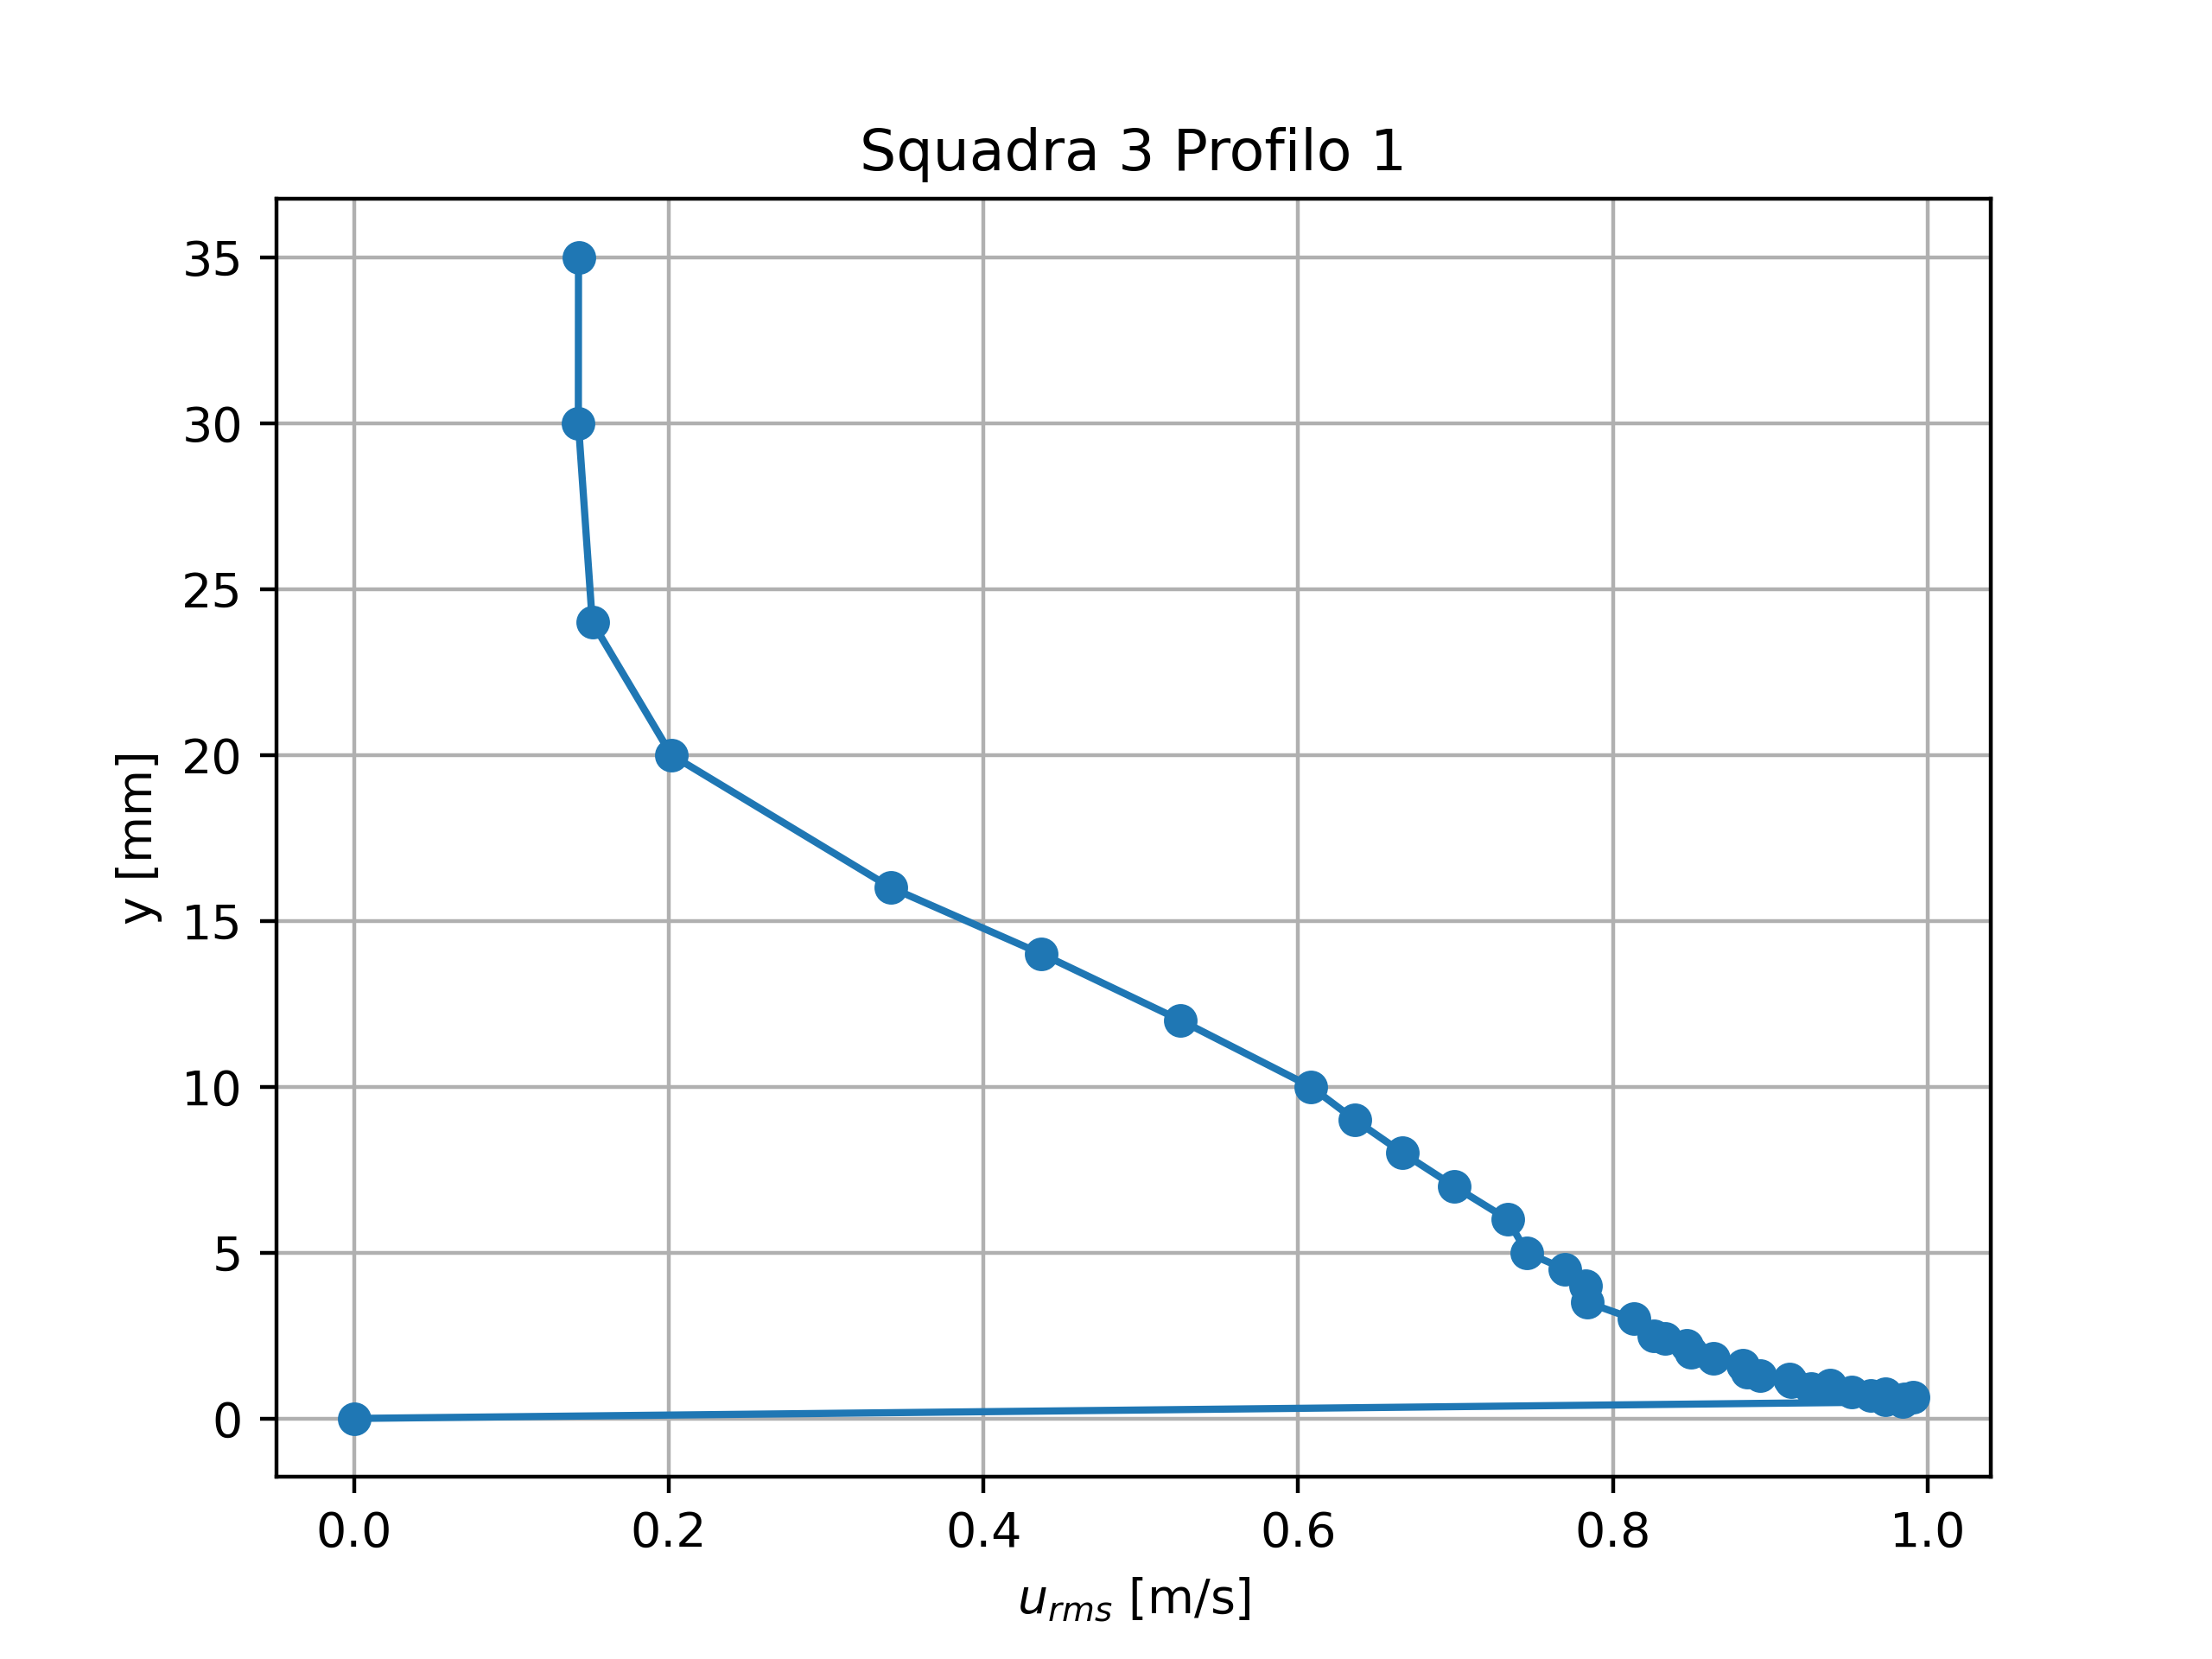
\includegraphics[width=.49\textwidth]{images/9/sq3p1rms.png}
    \caption{Esempi di profili di velocità e deviazione standard}
\end{figure}

\noindent Per stimare il valore di velocità a monte $U_\infty$, poiché per una placca piana la velocità a monte corrisponde alla velocità all'esterno dello strato limite $U_e$, si utilizzano i dati a disposizione della velocità $u(y)$, in particolare, si stima la velocità esterna dello strato limite $U_e$ come il massimo valore assunto da $u$ lungo $y$.\\\\
Mediante un'interpolazione lineare, è inoltre possibile stimare lo spessore geometrico dello strato limite $\delta(x)$, definito come la distanza da parete in cui la velocità assume il valore di $u=0.99U_e$.\\\\
Conoscendo la velocità esterna allo strato limite $U_e$ e lo spessore geometrico $\delta(x)$ è possibile diagrammare i profili di velocità in forma adimensionale $u/U_\infty=f(y/\delta)$:
\begin{figure}[H]
    \centering
    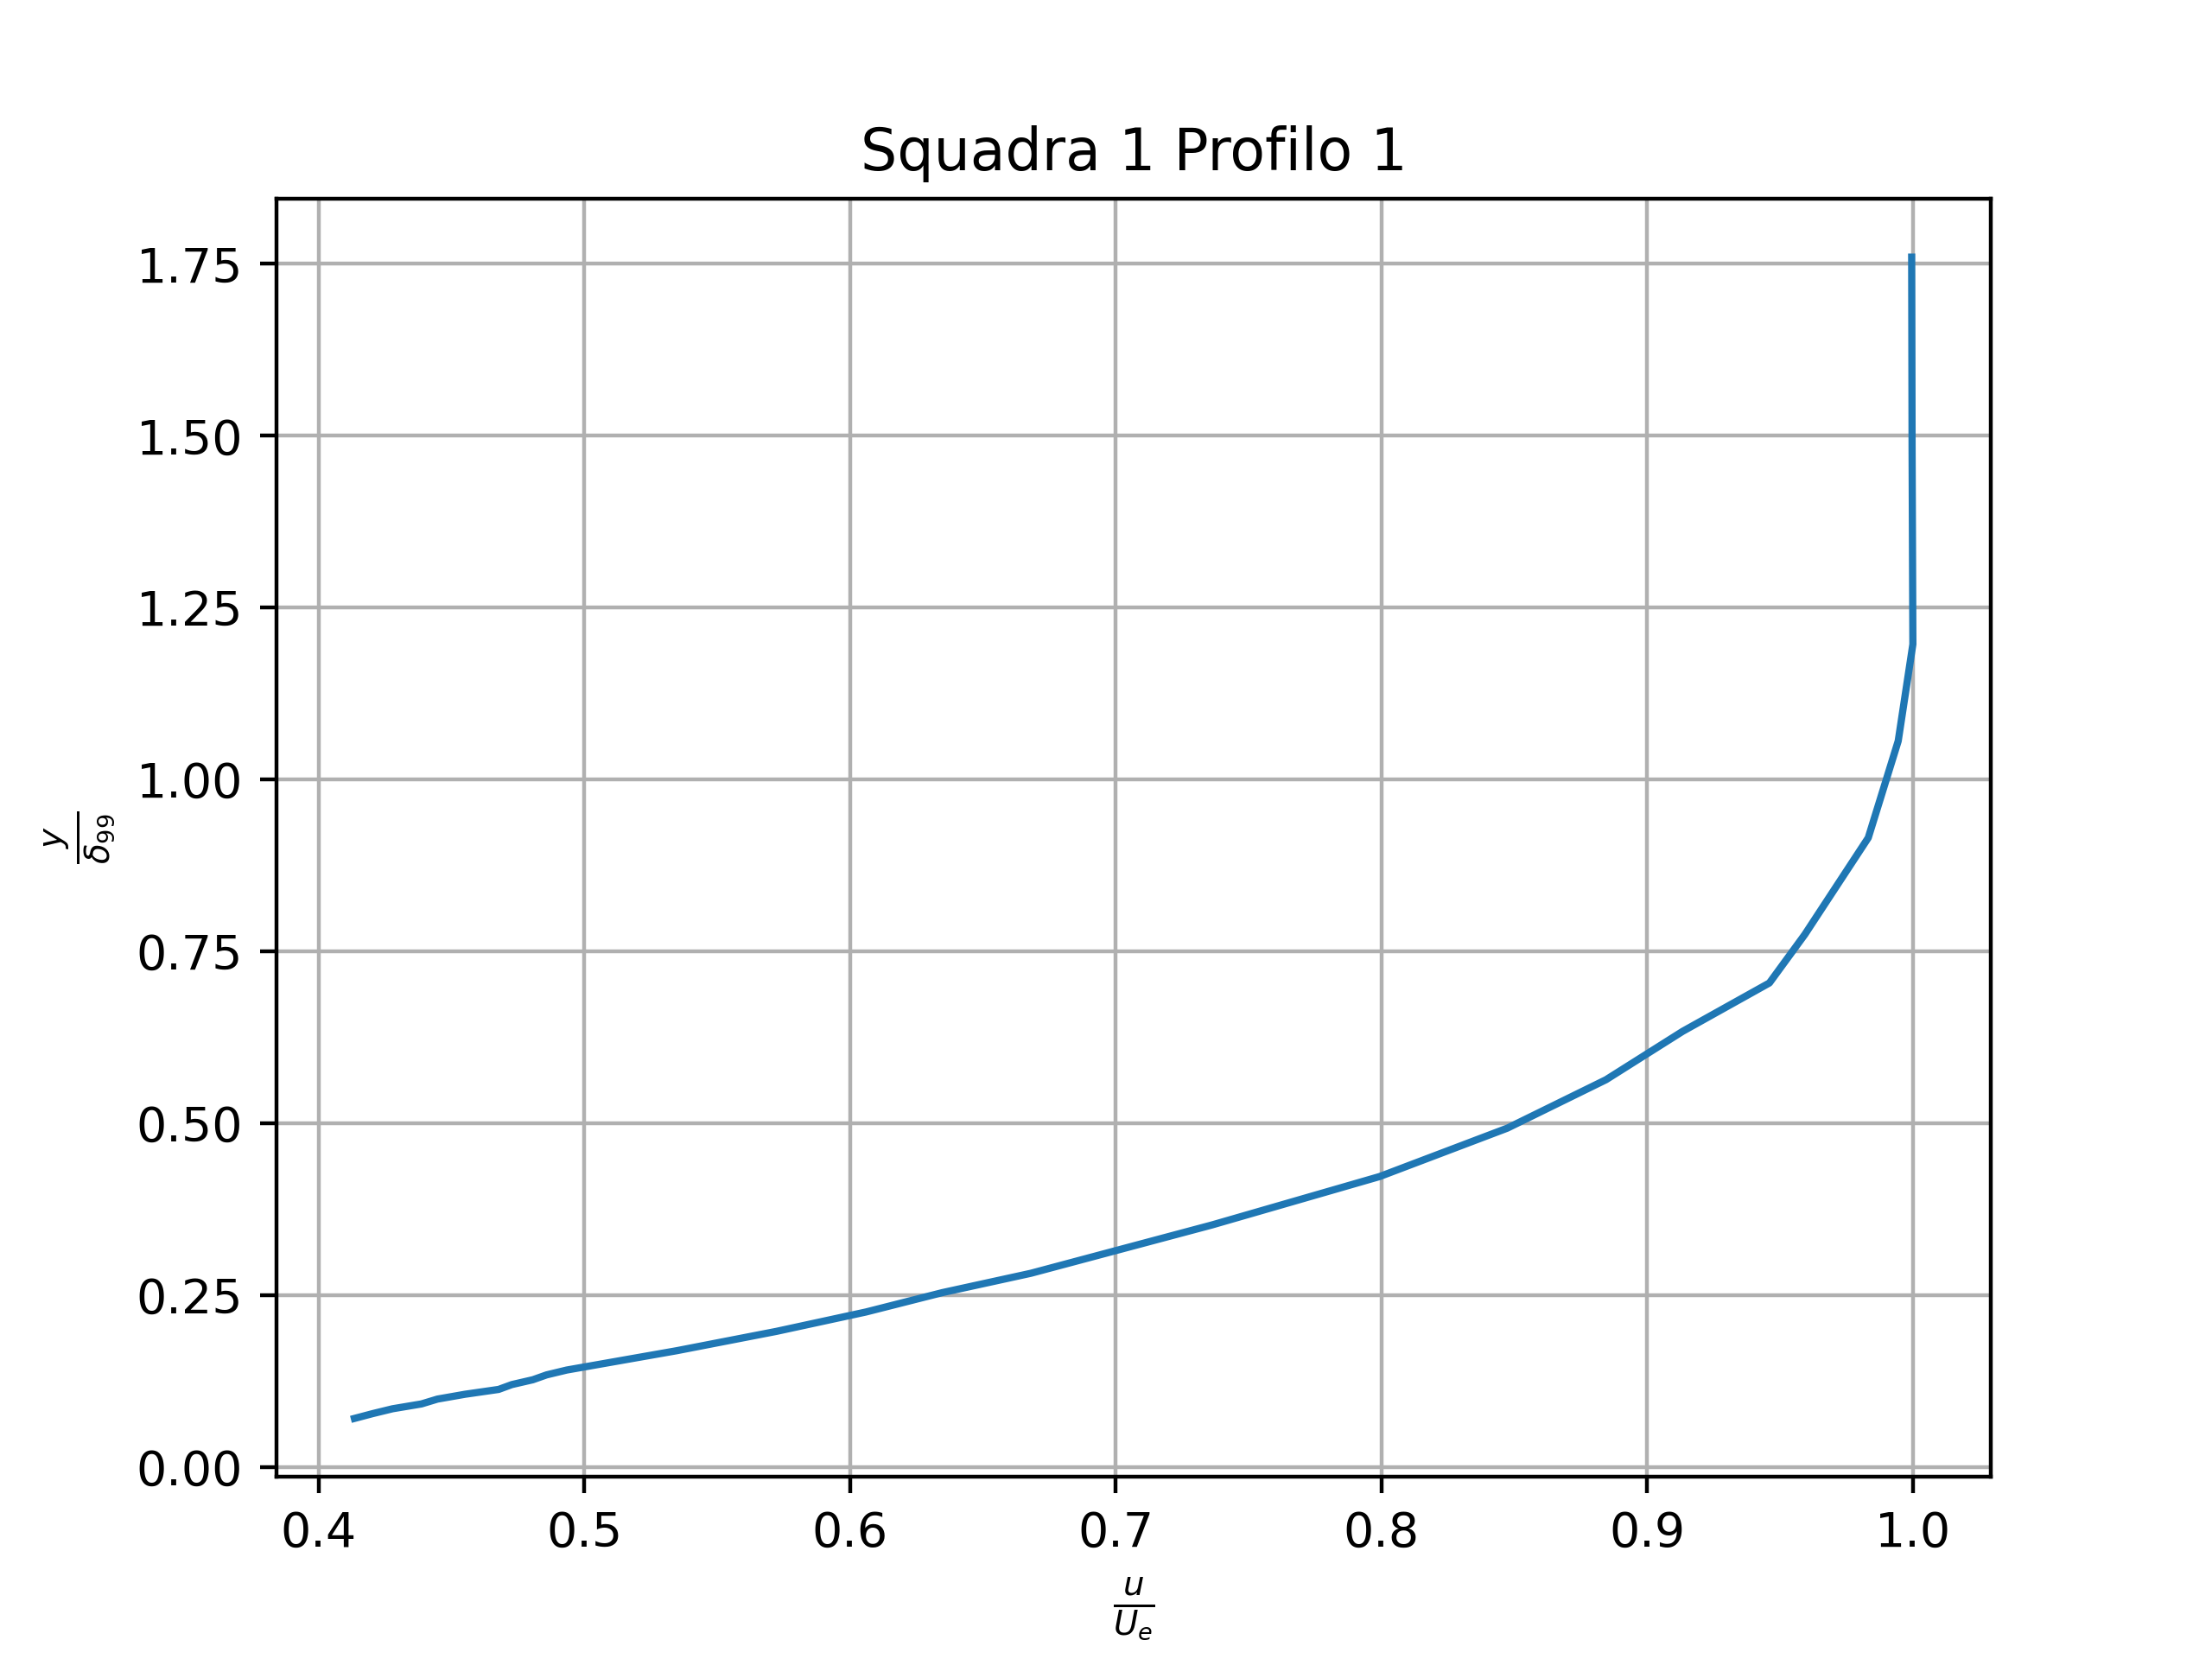
\includegraphics[width=.48\textwidth]{images/9/sq1p1_adim.png}
    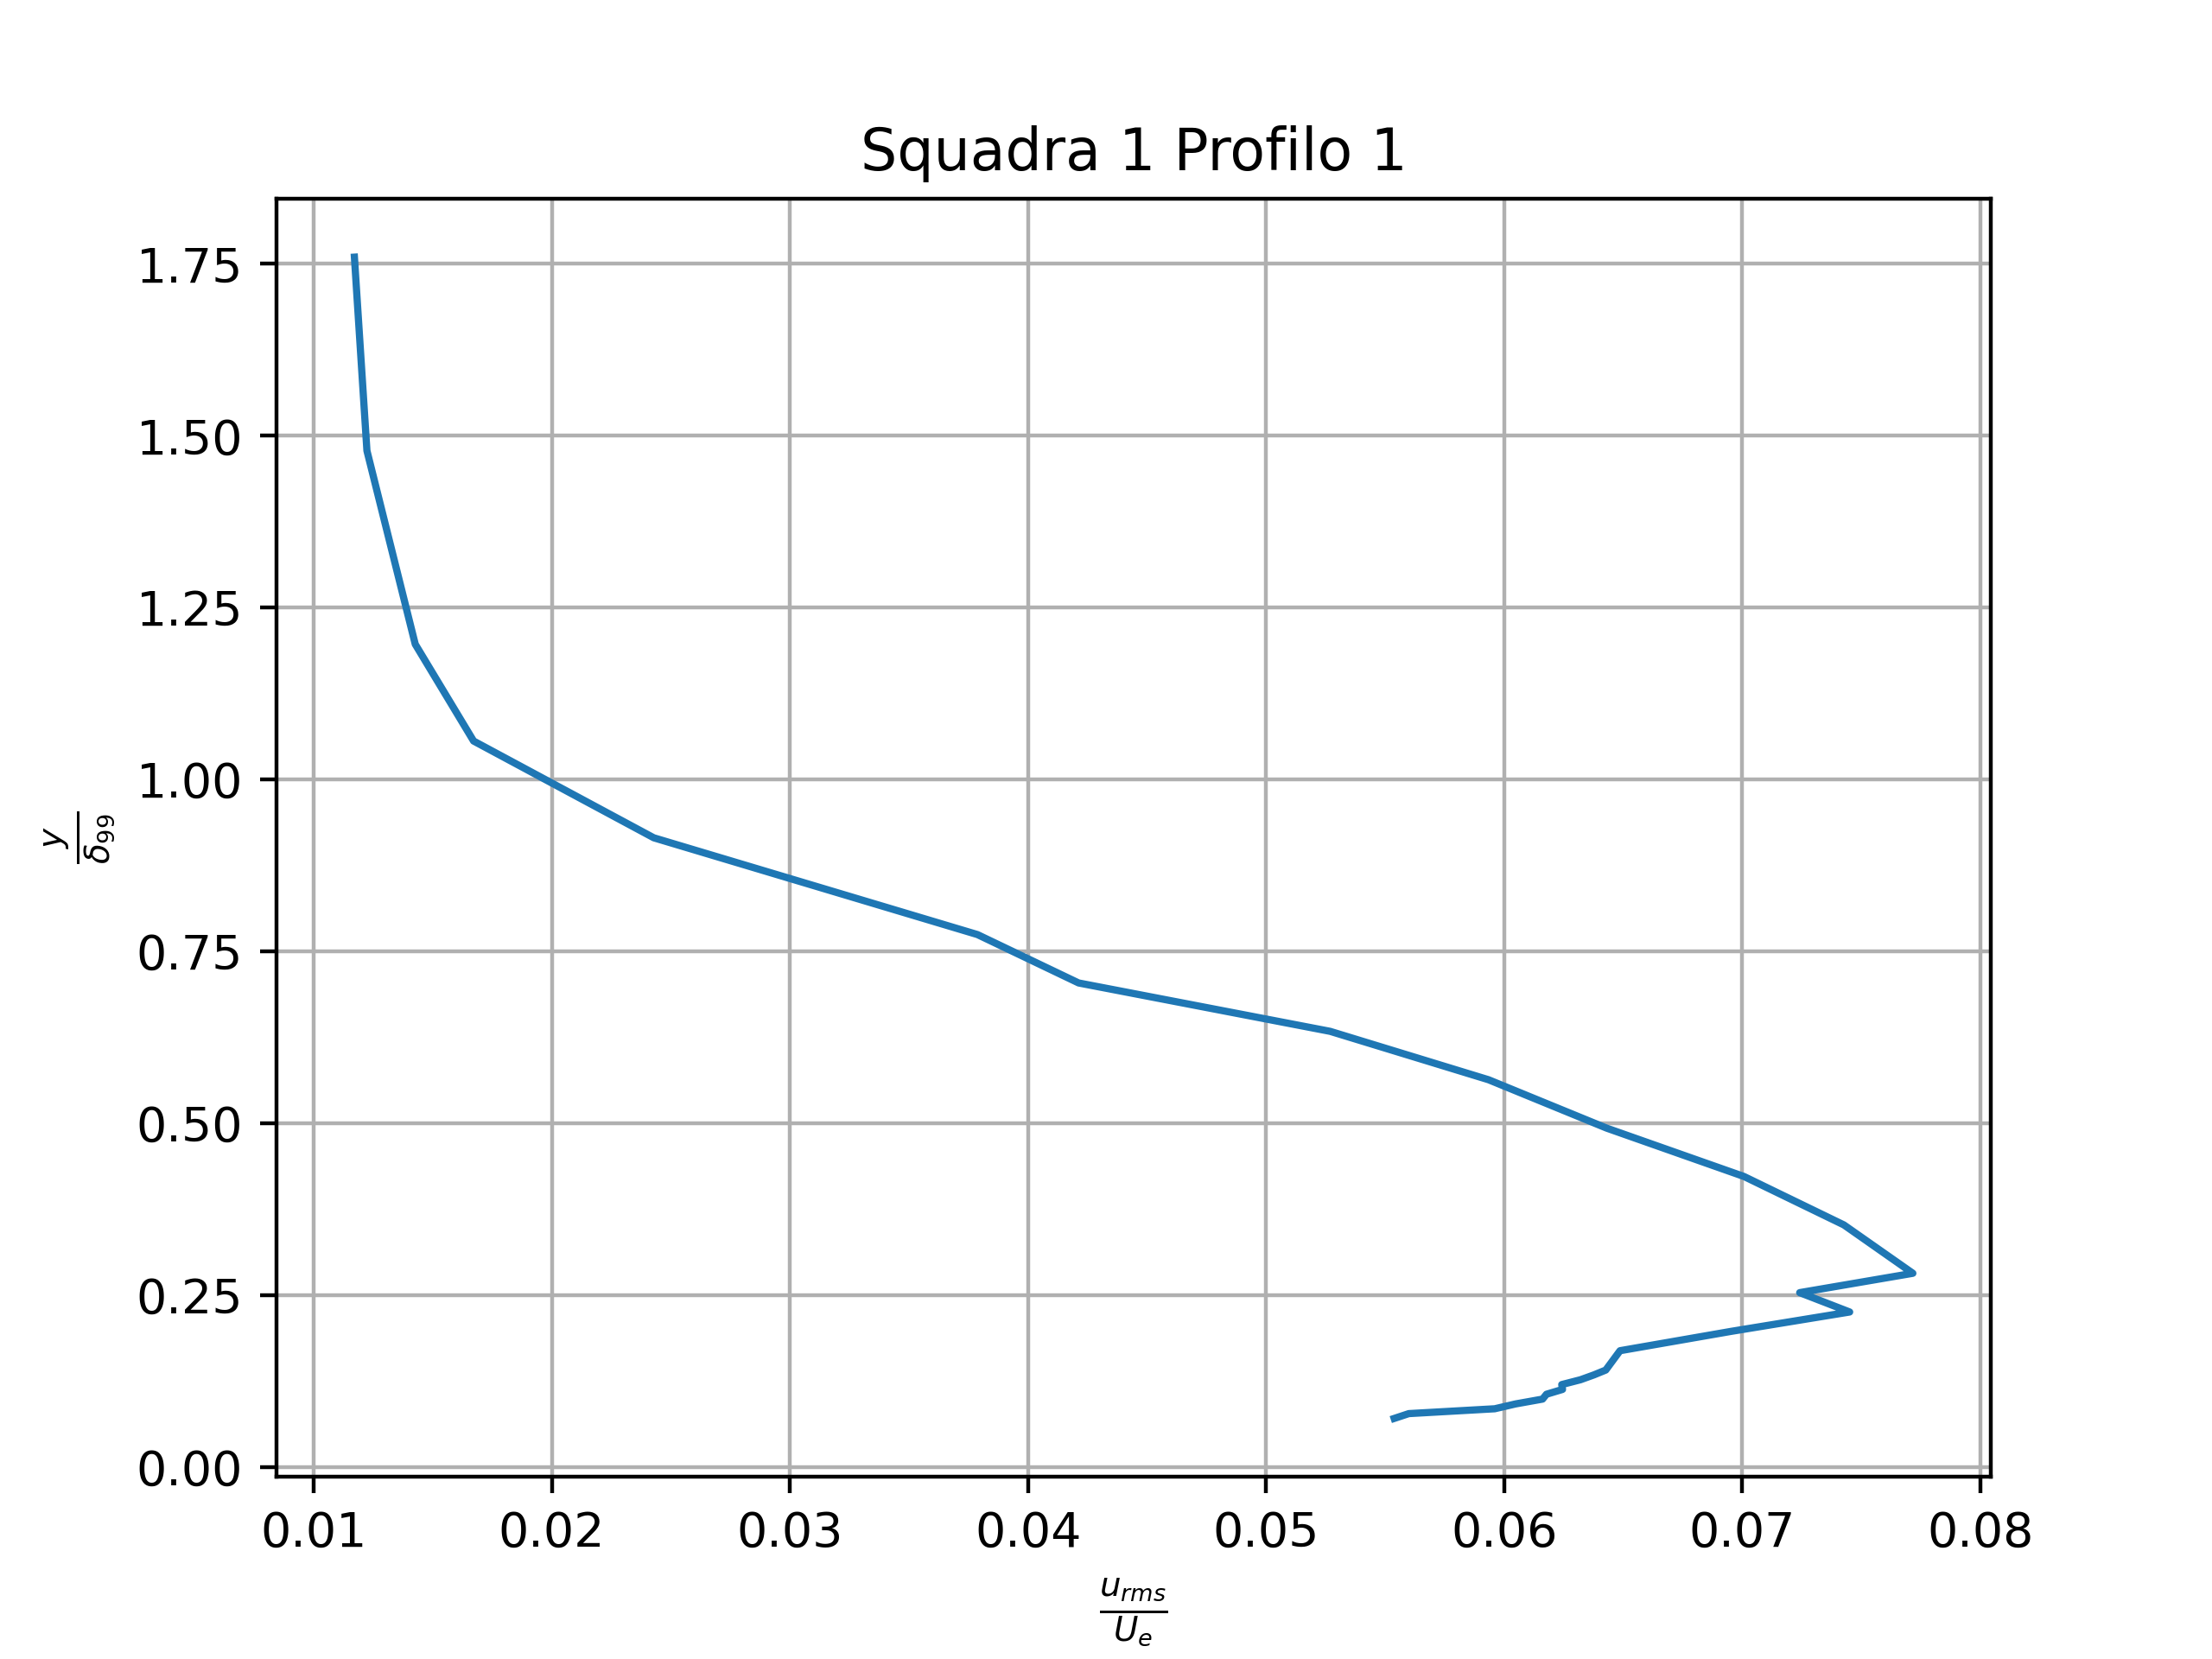
\includegraphics[width=.48\textwidth]{images/9/sq1p1_rms_adim.png}
    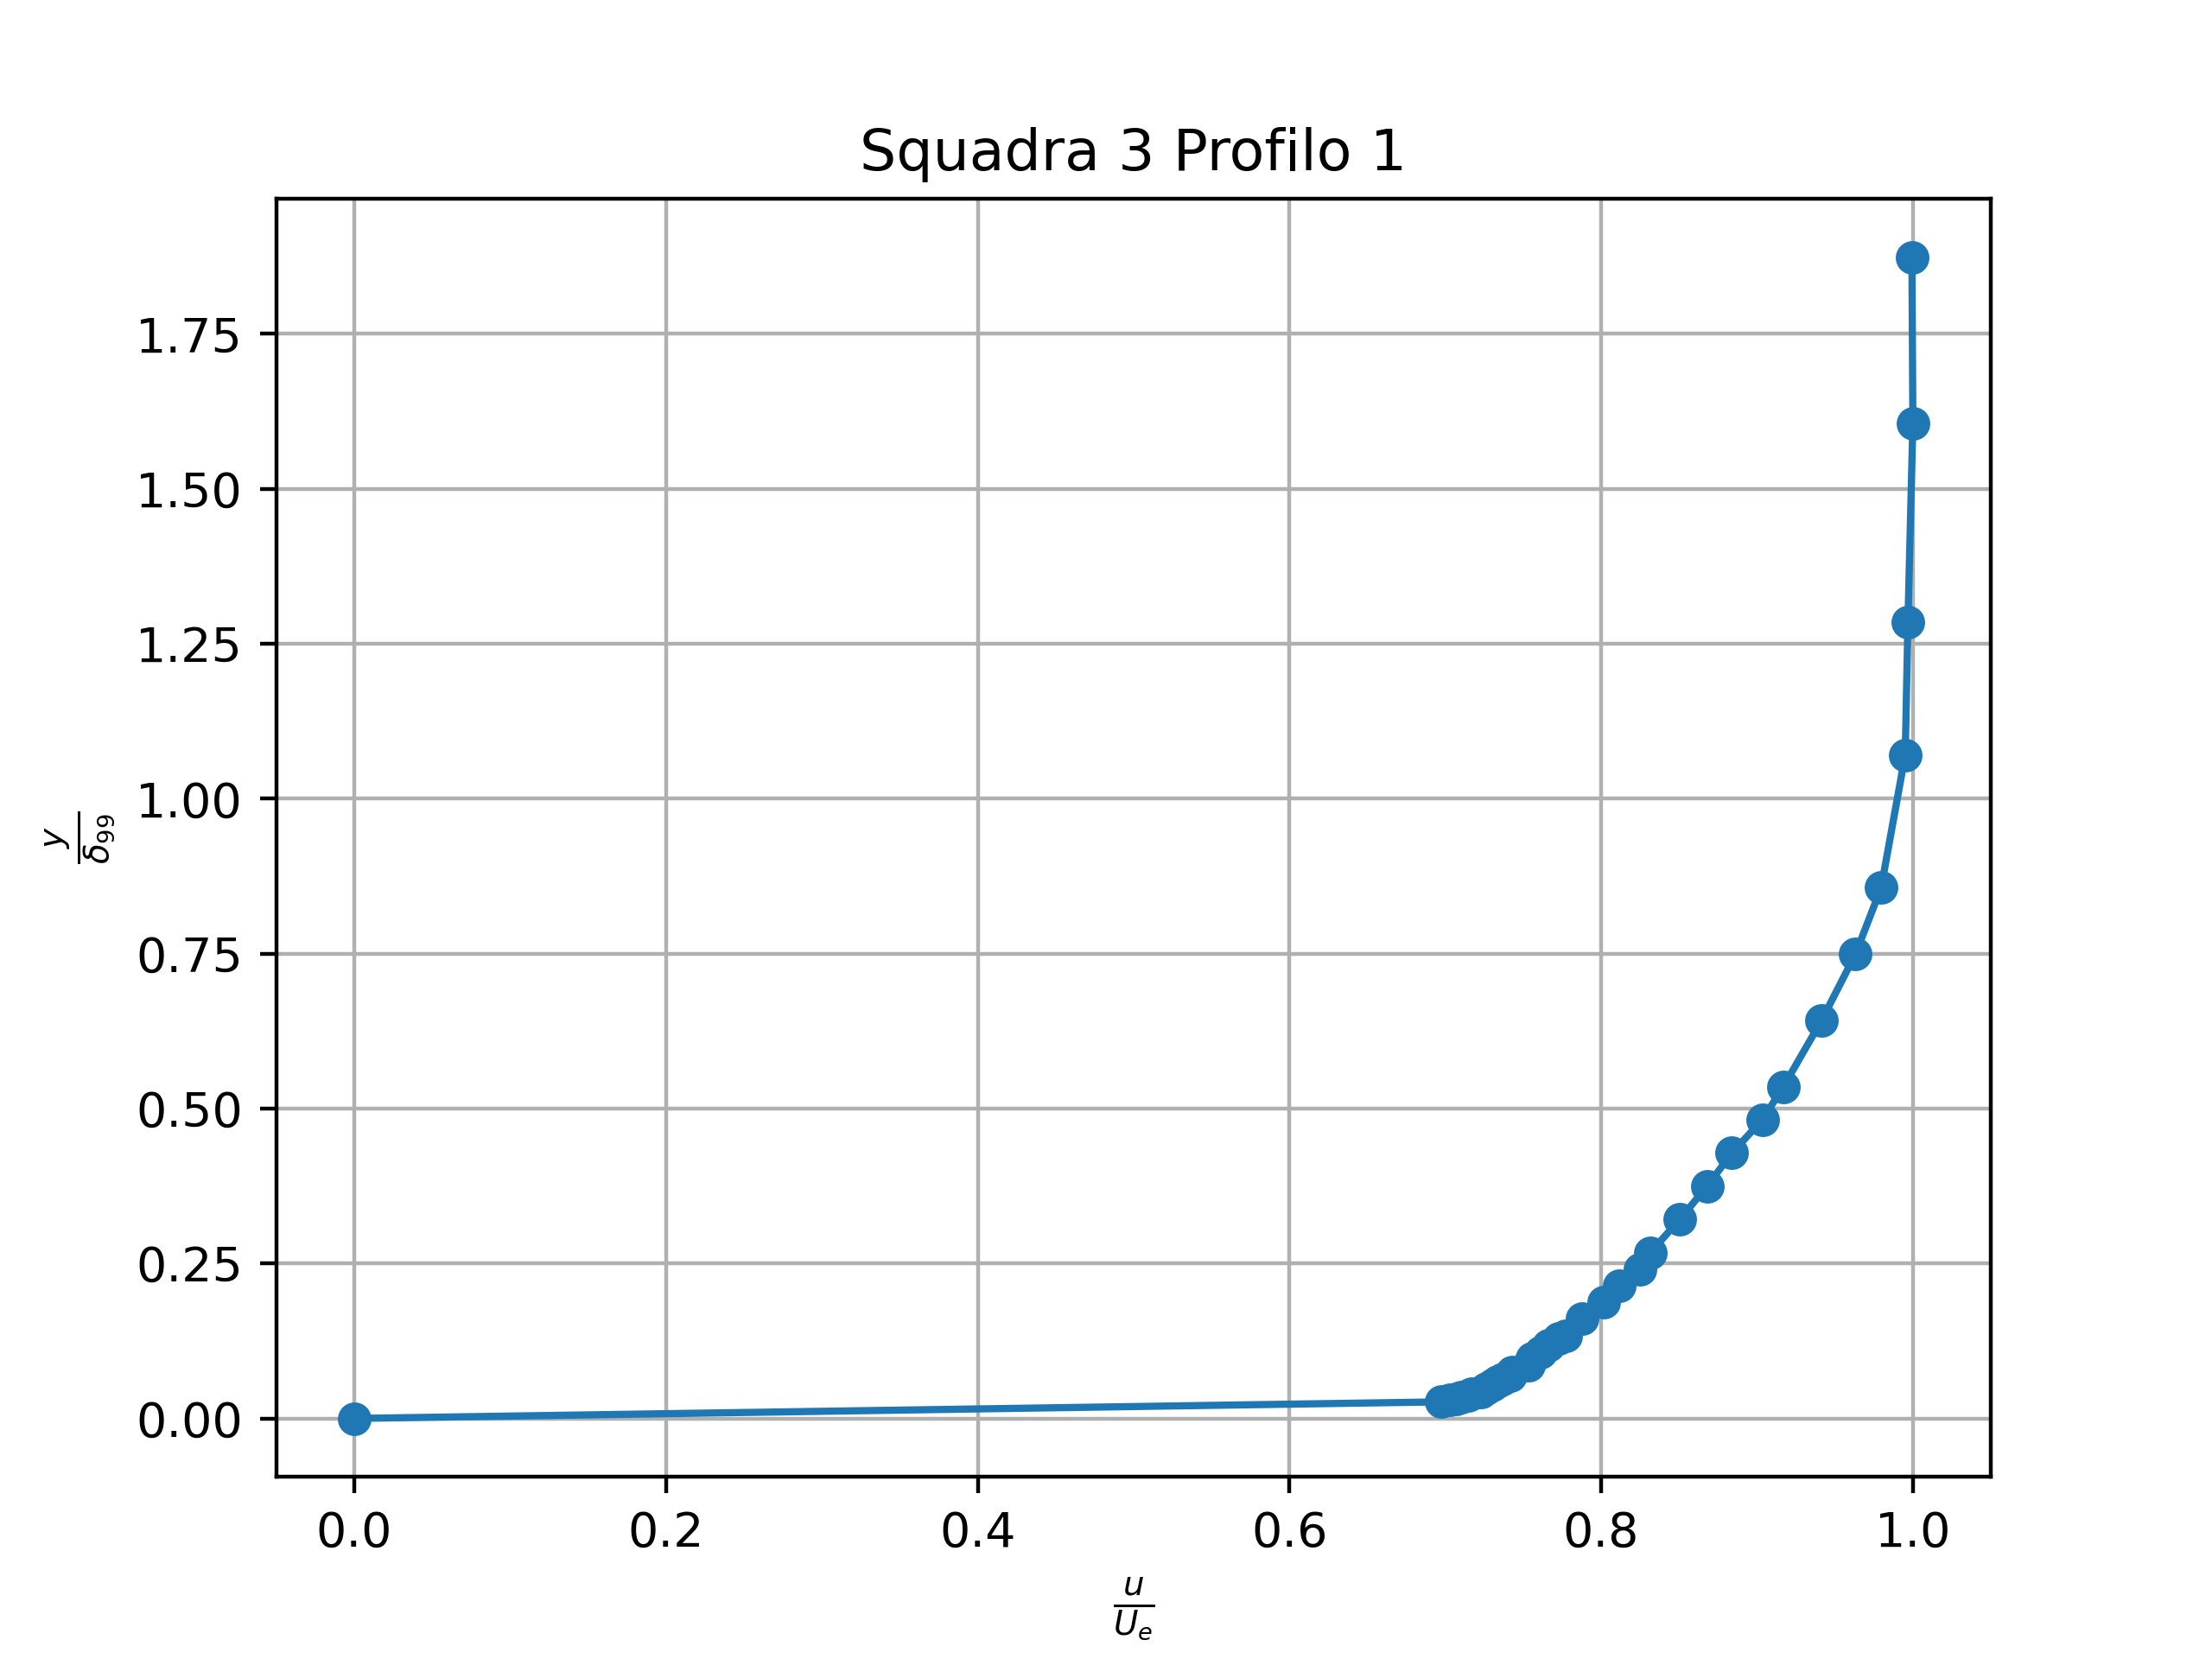
\includegraphics[width=.48\textwidth]{images/9/sq3p1_adim.png}
    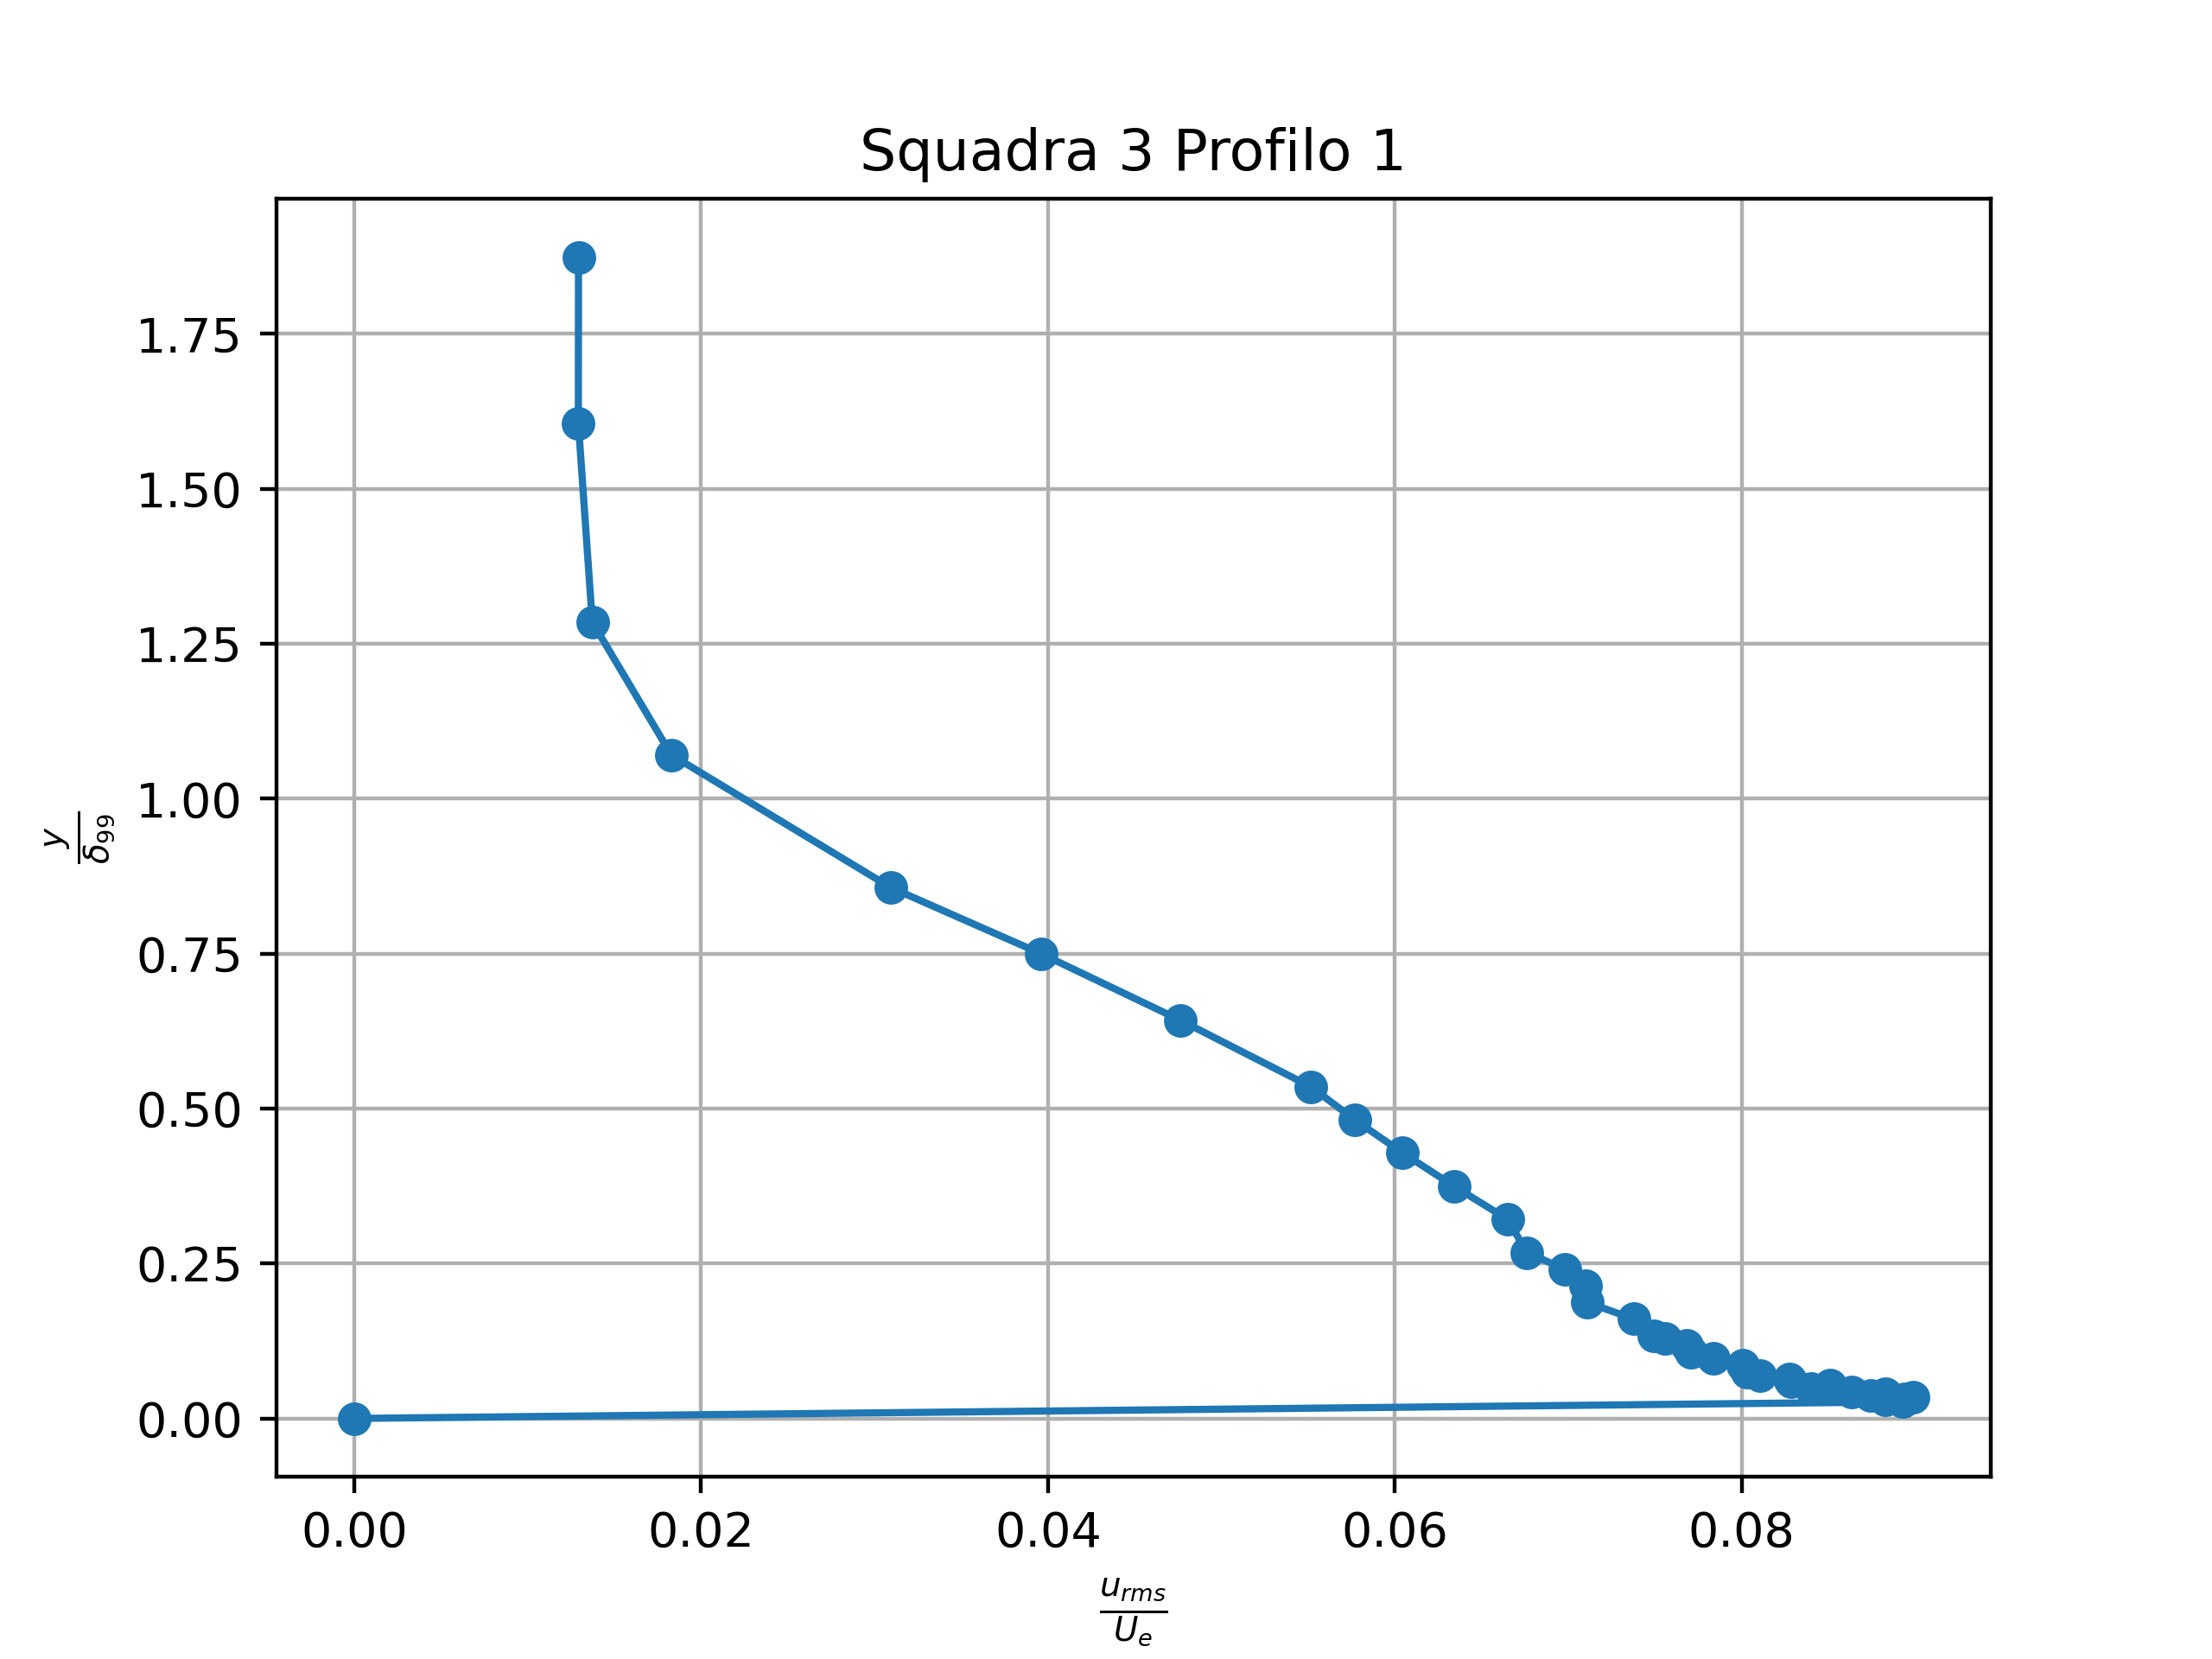
\includegraphics[width=.48\textwidth]{images/9/sq3p1_rms_adim.png}
    \caption{Esempi di profili di velocità e deviazione standard in forma adimensionale}
\end{figure}

\noindent Successivamente, si ricavano lo spessore di spostamento $\delta^*(x)$, lo spessore di quantità di moto $\theta(x)$ e il parametro di forma $H(x)$:
\begin{equation*}
    \delta^* = \int_0^\infty \left(1-\frac{u}{U_e}\right)dy \qquad \theta = \int_0^\infty \frac{u}{U_e}\left(1-\frac{u}{U_e}\right)dy \qquad H = \frac{\delta^*}{\theta}
\end{equation*}
Poiché si dispone di dati discreti, per gli integrali si utilizza la regola dei trapezi:
\begin{equation*}
    \int_a^b f(x)dx \approx \sum_{k=1}^n \frac{f(x_{k-1}) + f(x_k)}2 \Delta x_k \quad \text{con } \Delta x_k = x_k - x_{k-1}
\end{equation*}
Il metodo più immediato per determinare se lo strato limite analizzato è laminare, transizionale o turbolento, è il calcolo del numero di Reynolds locale $Re_x$, relativo alla coordinata $x$, se questo è maggiore del numero di Reynolds critico ($Re_{cr}\approx500000$) allora lo strato limite è turbolento, altrimenti è laminare:
\begin{equation*}
    Re_x = \frac{U_\infty x}\nu
\end{equation*}
Per le otto configurazioni, si ottengono i seguenti risultati:\\\\
\textbf{Squadra 1}\\
$-$ Profilo 1: $Re_x=316408\ \rightarrow\ $ strato limite laminare;\\
$-$ Profilo 2: $Re_x=521112\ \rightarrow\ $ strato limite turbolento;\\\\
\textbf{Squadra 2}\\
$-$ Profilo 1: $Re_x=358159\ \rightarrow\ $ strato limite laminare;\\
$-$ Profilo 2: $Re_x=649986\ \rightarrow\ $ strato limite turbolento;\\\\
\textbf{Squadra 3}\\
$-$ Profilo 1: $Re_x=656506\ \rightarrow\ $ strato limite turbolento;\\
$-$ Profilo 2: $Re_x=214079\ \rightarrow\ $ strato limite laminare;\\\\
\textbf{Squadra 4}\\
$-$ Profilo 1: $Re_x=143967\ \rightarrow\ $ strato limite laminare;\\
$-$ Profilo 2: $Re_x=498714\ \rightarrow\ $ strato limite transizionale;\\\\
Un altro parametro utile a determinare il regime dello strato limite è il parametro di forma $H(x)$. Questo infatti assume un valore $H\approx2.59$ (soluzione di Blasius) nel caso di strato limite laminare, mentre assume un valore attorno a $H\approx1.3$ nel caso di strato limite turbolento.\\\\
Si ottengono i seguenti risultati per le grandezze caratteristiche dello strato limite per le otto configurazioni: 
\begin{table}[H]
    \centering
    \begin{tabular}{|c|c|c|c|c|c|}
    \hline
    Configurazione             & $Re_x$ & $\delta_{99}$ & $\delta^*$ & $\theta$ & $H$  \\ \hline
    Squadra 1 Profilo 1 & 316408 & 7.10 mm     & 1.26 mm    & 0.83 mm  & 1.52 \\ \hline
    Squadra 1 Profilo 2 & 521112 & 21.19 mm    & 2.07 mm    & 1.72 mm  & 1.20 \\ \hline
    Squadra 2 Profilo 1 & 358159 & 6.53 mm     & 1.53 mm    & 0.79 mm  & 1.92 \\ \hline
    Squadra 2 Profilo 2 & 649986 & 21.17 mm    & 2.45 mm    & 1.81 mm  & 1.35 \\ \hline
    Squadra 3 Profilo 1 & 656506 & 18.68 mm    & 2.31 mm    & 1.72 mm  & 1.35 \\ \hline
    Squadra 3 Profilo 2 & 214079 & 15.81 mm    & 3.93 mm    & 1.96 mm  & 2.01 \\ \hline
    Squadra 4 Profilo 1 & 143967 & 17.17 mm    & 5.11 mm    & 2.06 mm  & 2.48 \\ \hline
    Squadra 4 Profilo 2 & 498714 & 13.50 mm    & 1.96 mm    & 1.32 mm  & 1.48 \\ \hline
    \end{tabular}
\end{table}

\noindent Si evince che il parametro di forma in alcune configurazioni non rispetta la considerazione teorica precedentemente espressa. Questo è dovuto al fatto che in alcune configurazioni lo strato limite è transizionale, e presenta pertanto turbolenza intermittente. Si osserva inoltre come lo spessore geometrico $\delta_{99}$ dello strato limite sia fortemente influenzato dalla distanza $x$ dal bordo di attacco della placca piana (lo spessore dello strato limite aumenta lungo la placca piana).\\\\
\noindent È opportuno confrontare i risultati ottenuti con le soluzioni empiriche:
\begin{table}[H]
    \centering
    \begin{tabular}{|c|c|c|c|c|c|}
    \hline
    Configurazione             & $Re_x$ & $\delta_{99,emp}$ & $\delta^*_{emp}$ & $\theta_{emp}$ & $H_{emp}$ \\ \hline
    Squadra 1 Profilo 1 & 316408 & 4.89 mm           & 1.69 mm          & 0.65 mm        & 2.61      \\ \hline
    Squadra 1 Profilo 2 & 521112 & 23.94 mm          & 2.99 mm          & 2.33 mm        & 1.28      \\ \hline
    Squadra 2 Profilo 1 & 358159 & 4.18 mm           & 1.45 mm          & 0.55 mm        & 2.61      \\ \hline
    Squadra 2 Profilo 2 & 649986 & 22.90 mm          & 2.86 mm          & 2.23 mm        & 1.28      \\ \hline
    Squadra 3 Profilo 1 & 656506 & 22.86 mm          & 2.86 mm          & 2.22 mm        & 1.28      \\ \hline
    Squadra 3 Profilo 2 & 214079 & 9.73 mm           & 3.37 mm          & 1.29 mm        & 2.61      \\ \hline
    Squadra 4 Profilo 1 & 143967 & 9.22 mm           & 3.19 mm          & 1.22 mm        & 2.61      \\ \hline
    Squadra 4 Profilo 2 & 498714 & 18.78 mm          & 2.35 mm          & 1.83 mm        & 1.28      \\ \hline
    \end{tabular}
\end{table}

\noindent Come già accennato, i dati risultanti delle formulazioni empiriche per alcune configurazioni si discostano dai risultati sperimentali per via del regime transizionale dello strato limite.

\subsubsection{Strato limite laminare}
Nel caso di strato limite laminare la soluzione delle equazioni porta alla soluzione esatta di Blasius, che definisce il profilo di velocità in forma adimensionale:
\begin{equation*}
    \eta(x,y) = y\sqrt{\frac{U_\infty}{\nu x}} \qquad \phi = \frac{u}{U_\infty}
\end{equation*}
È opportuno confrontare la teoria di Blasius con i risultati sperimentali ottenuti. Si ottengono quindi i seguenti diagrammi:
\begin{figure}[H]
    \centering
    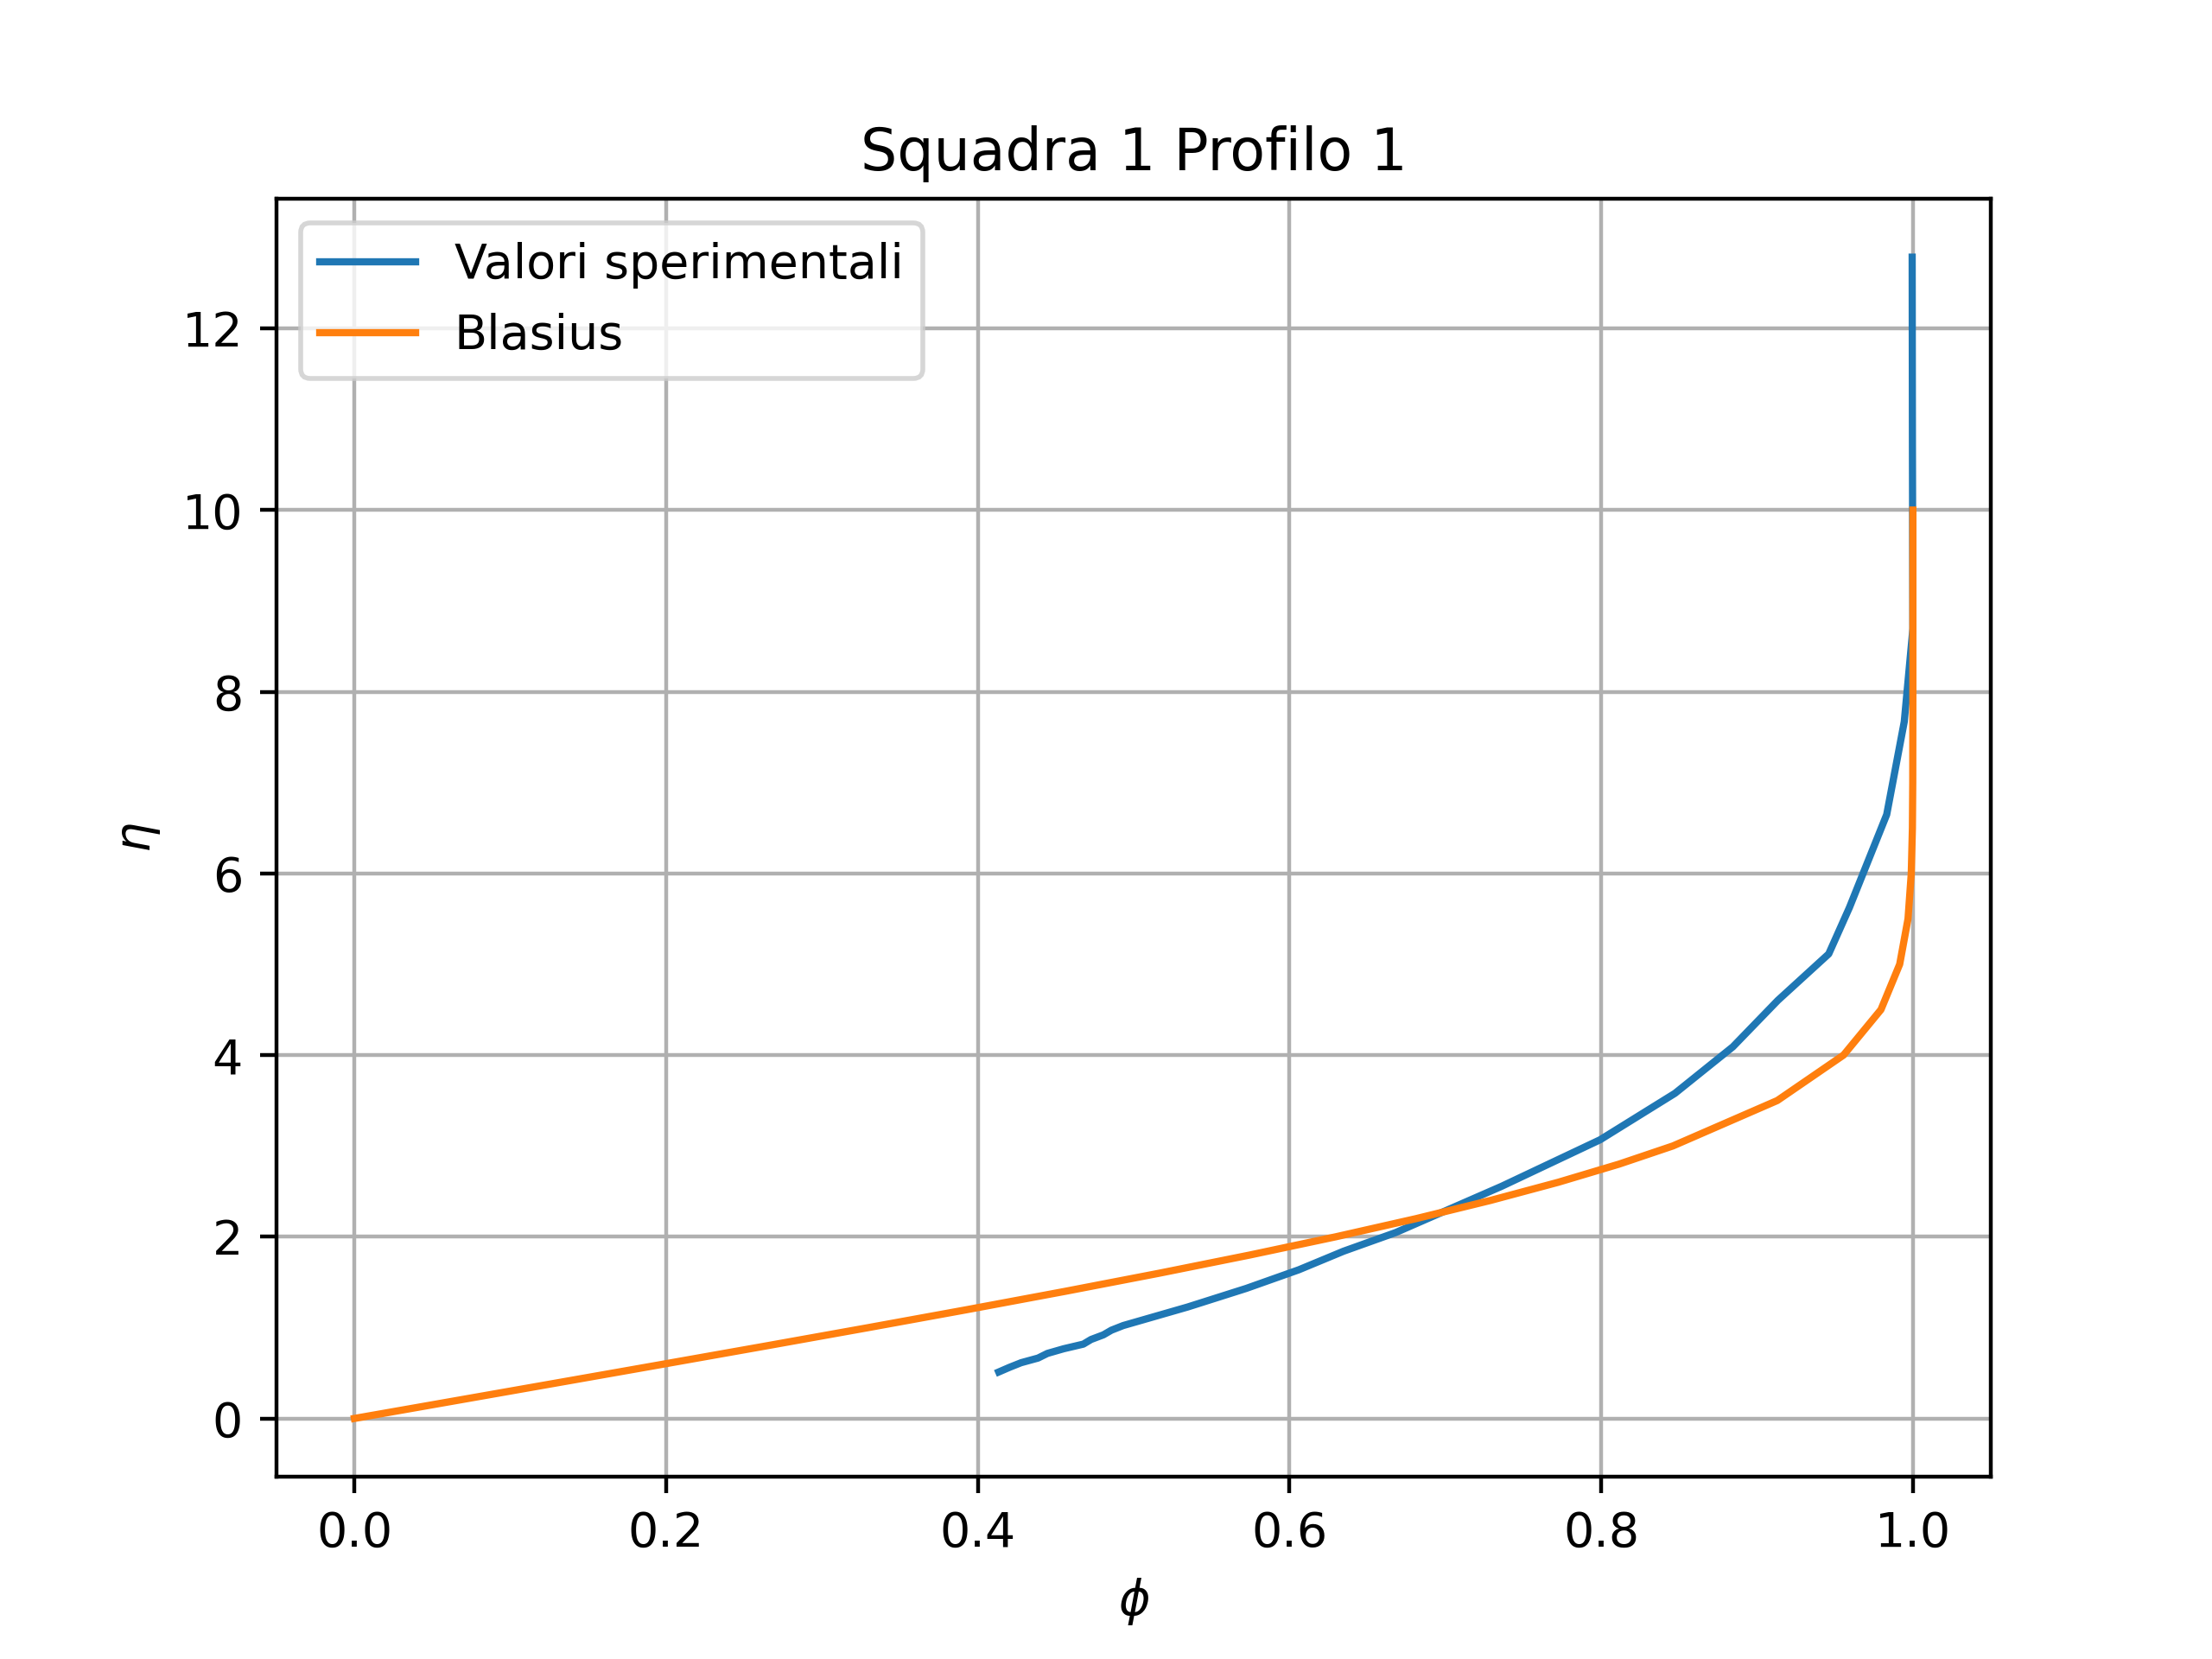
\includegraphics[width=.49\textwidth]{images/9/sq1p1_blasius.png}
    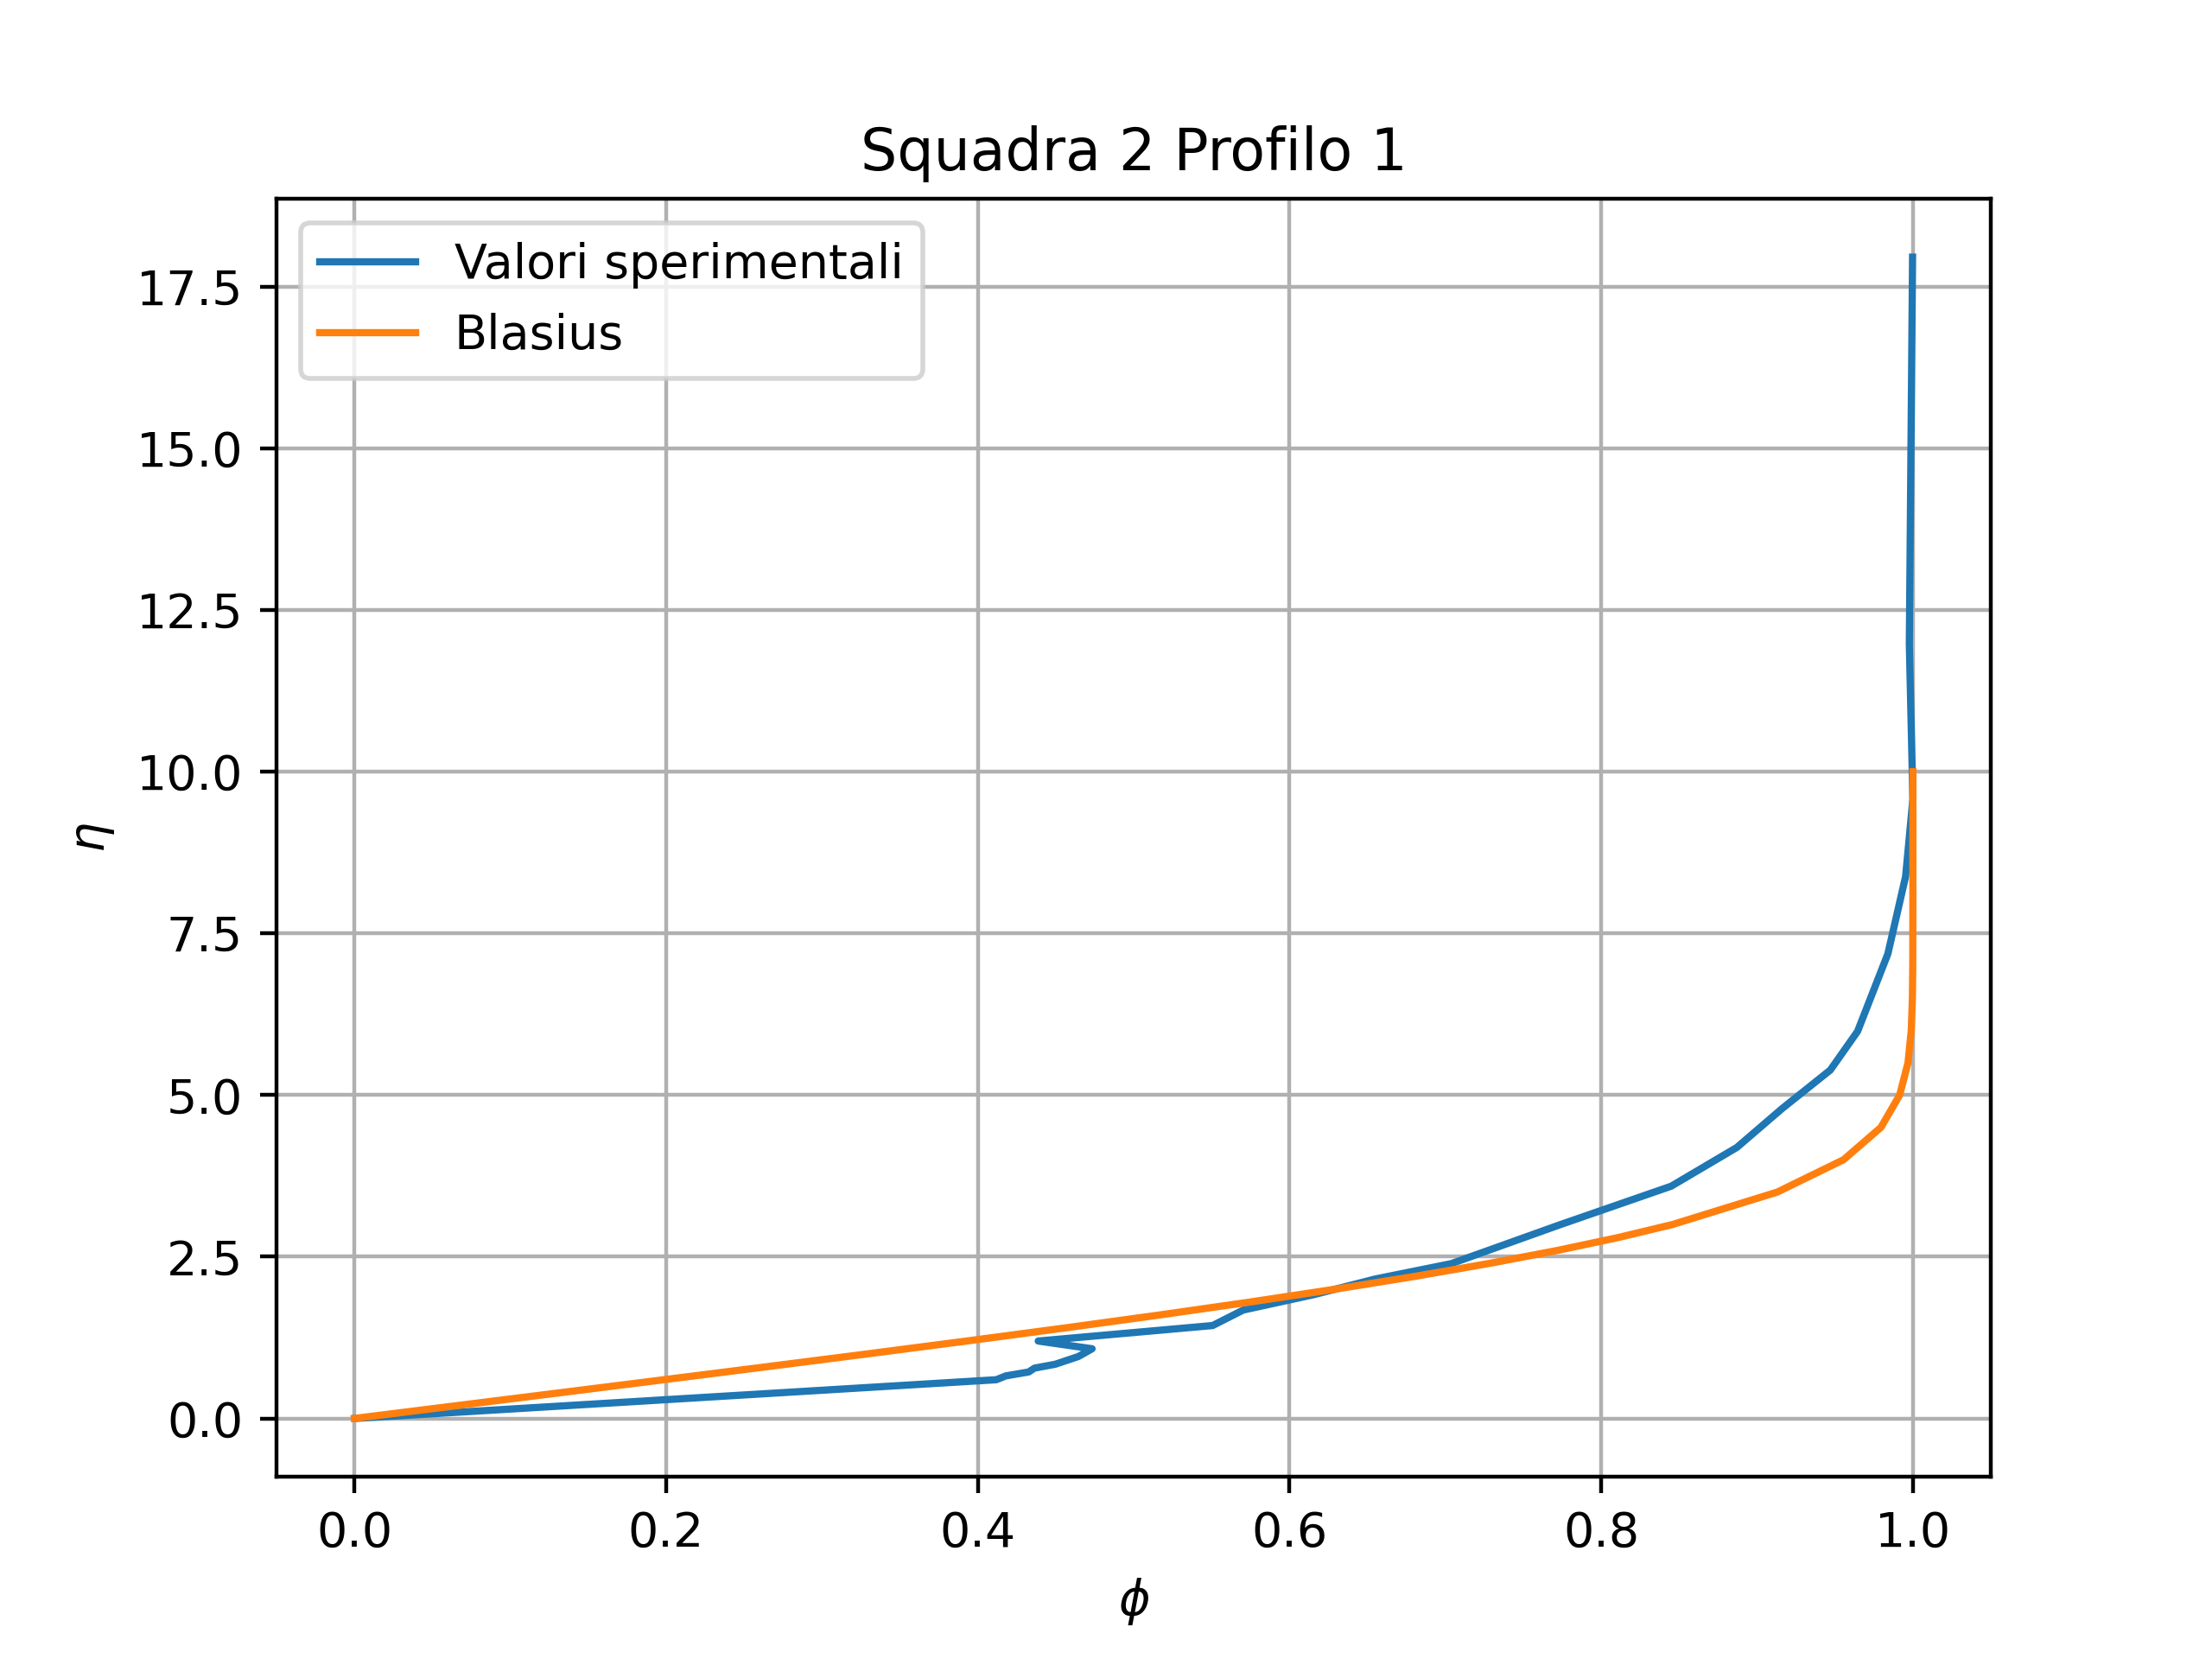
\includegraphics[width=.49\textwidth]{images/9/sq2p1_blasius.png}
    \caption{Confronto con la soluzione di Blasius, squadre 1 e 2}
\end{figure}

\begin{figure}[H]
    \centering
    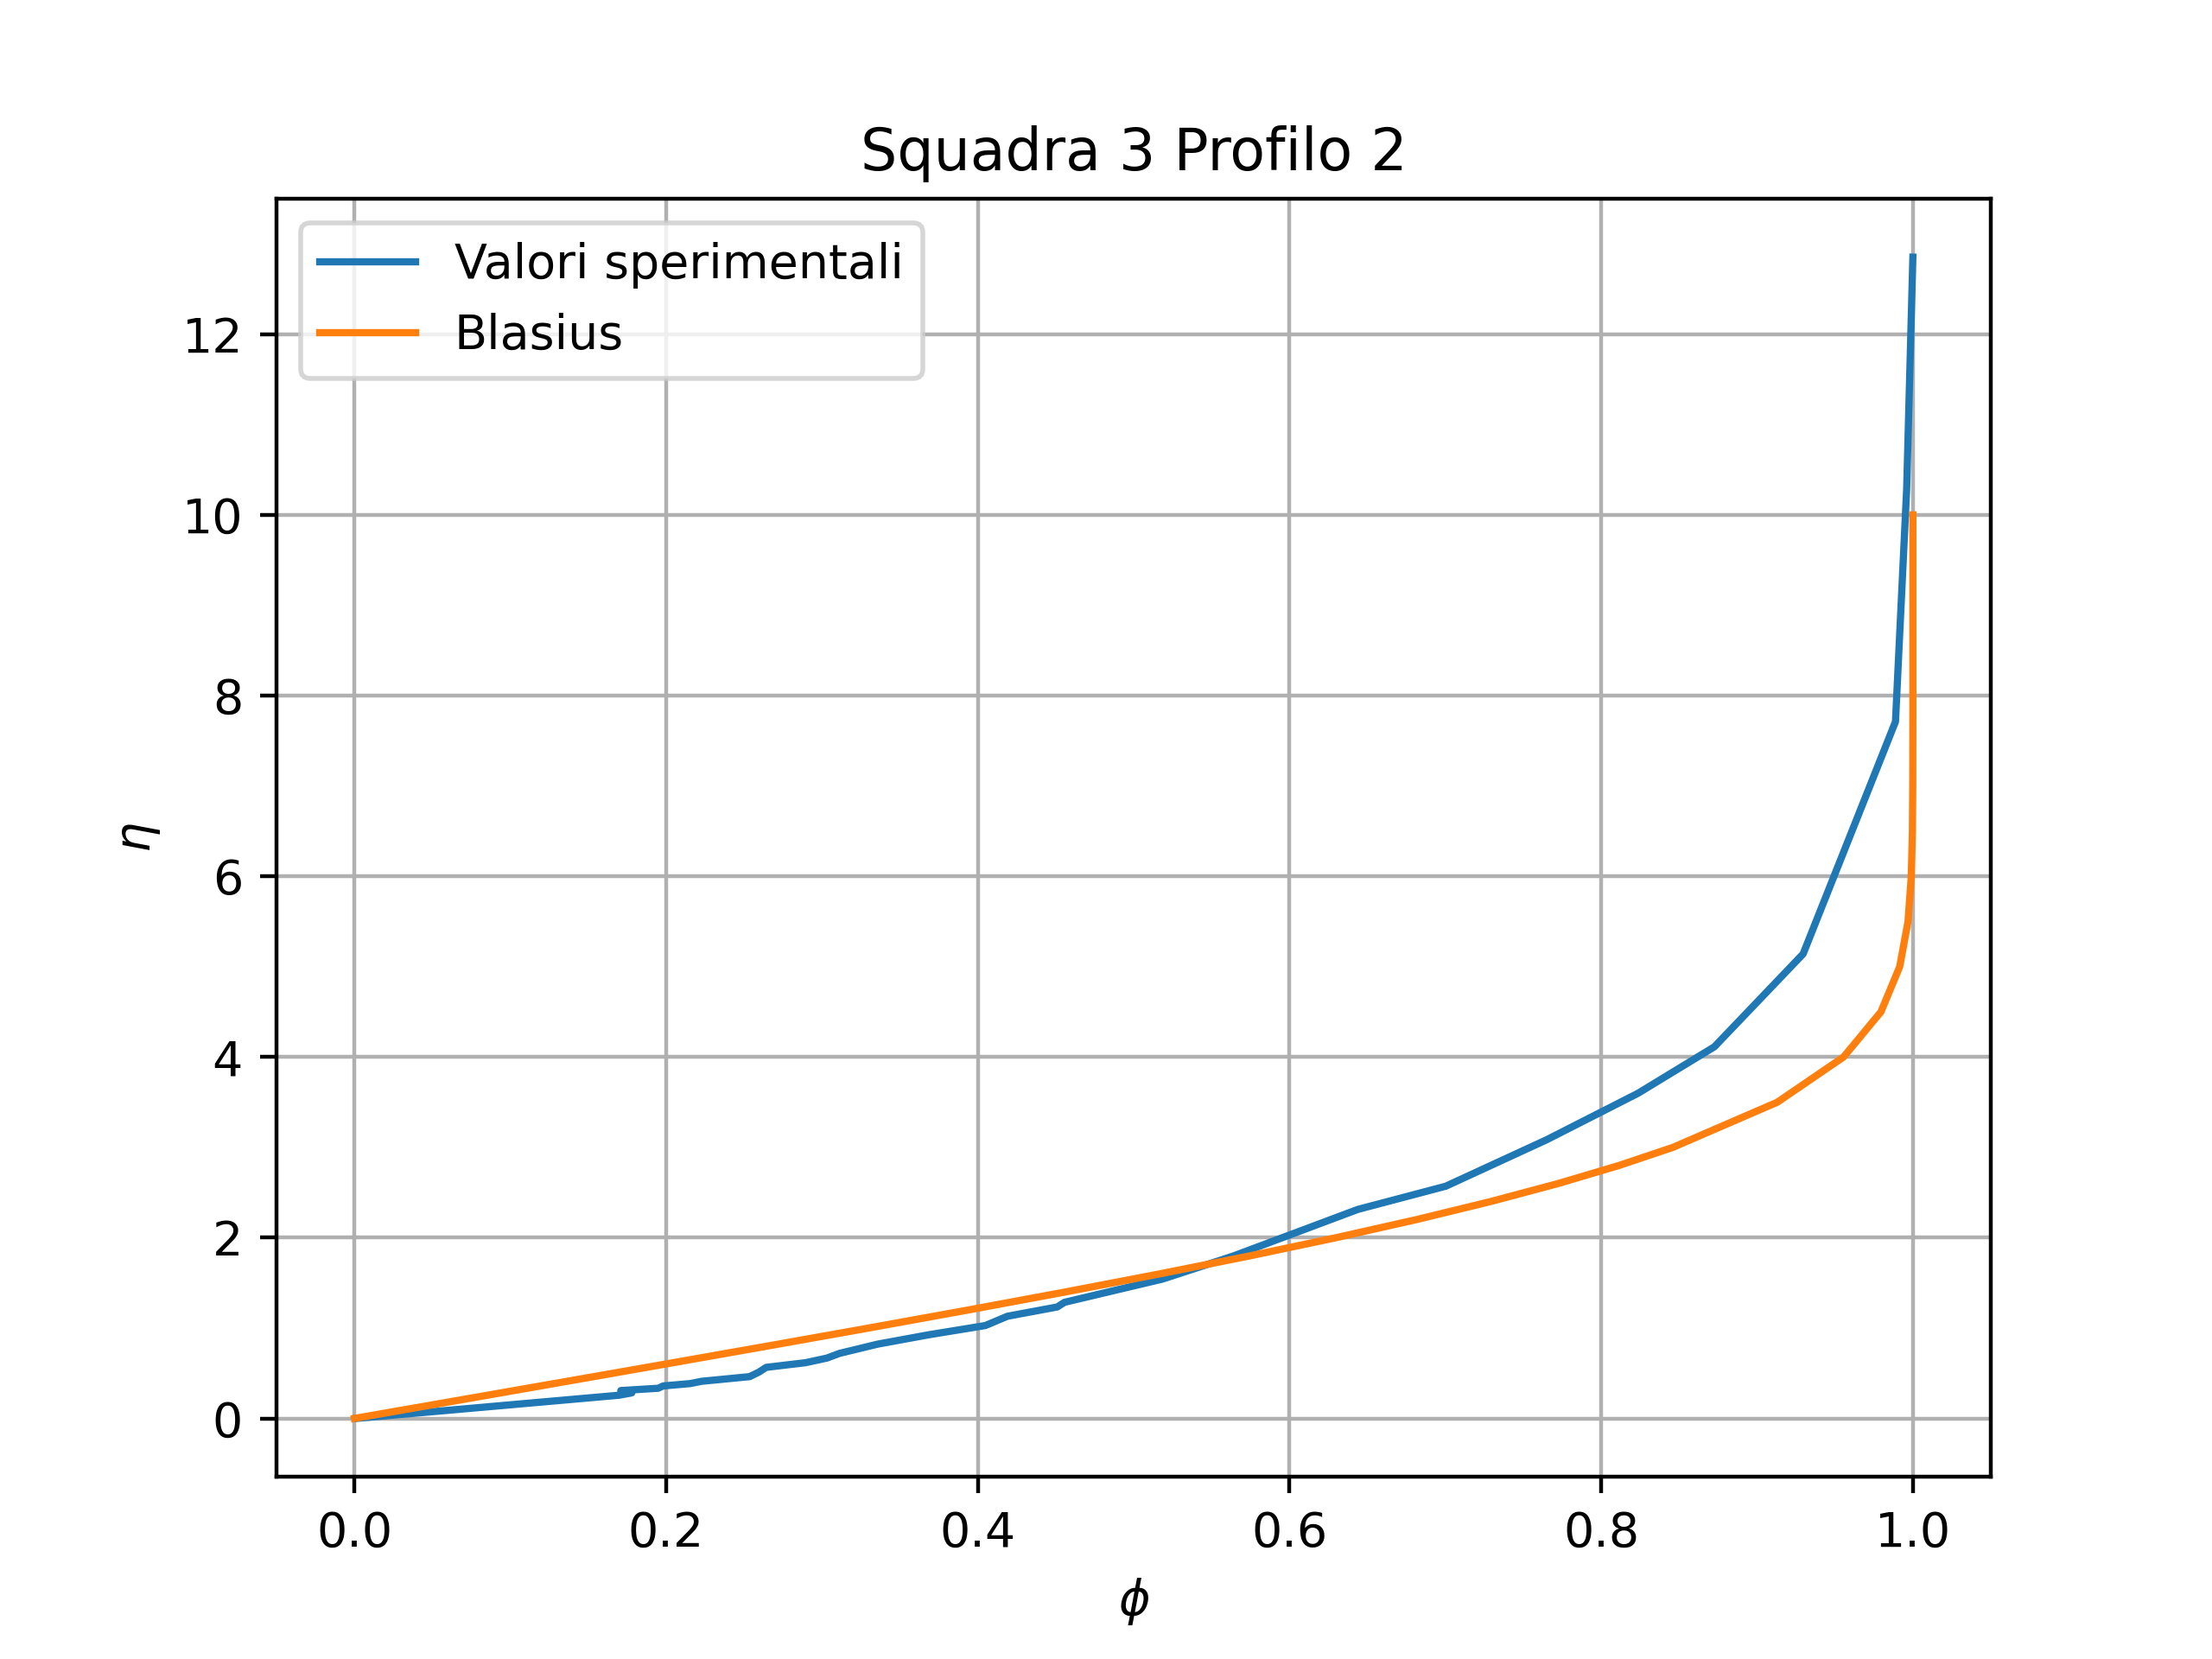
\includegraphics[width=.49\textwidth]{images/9/sq3p2_blasius.png}
    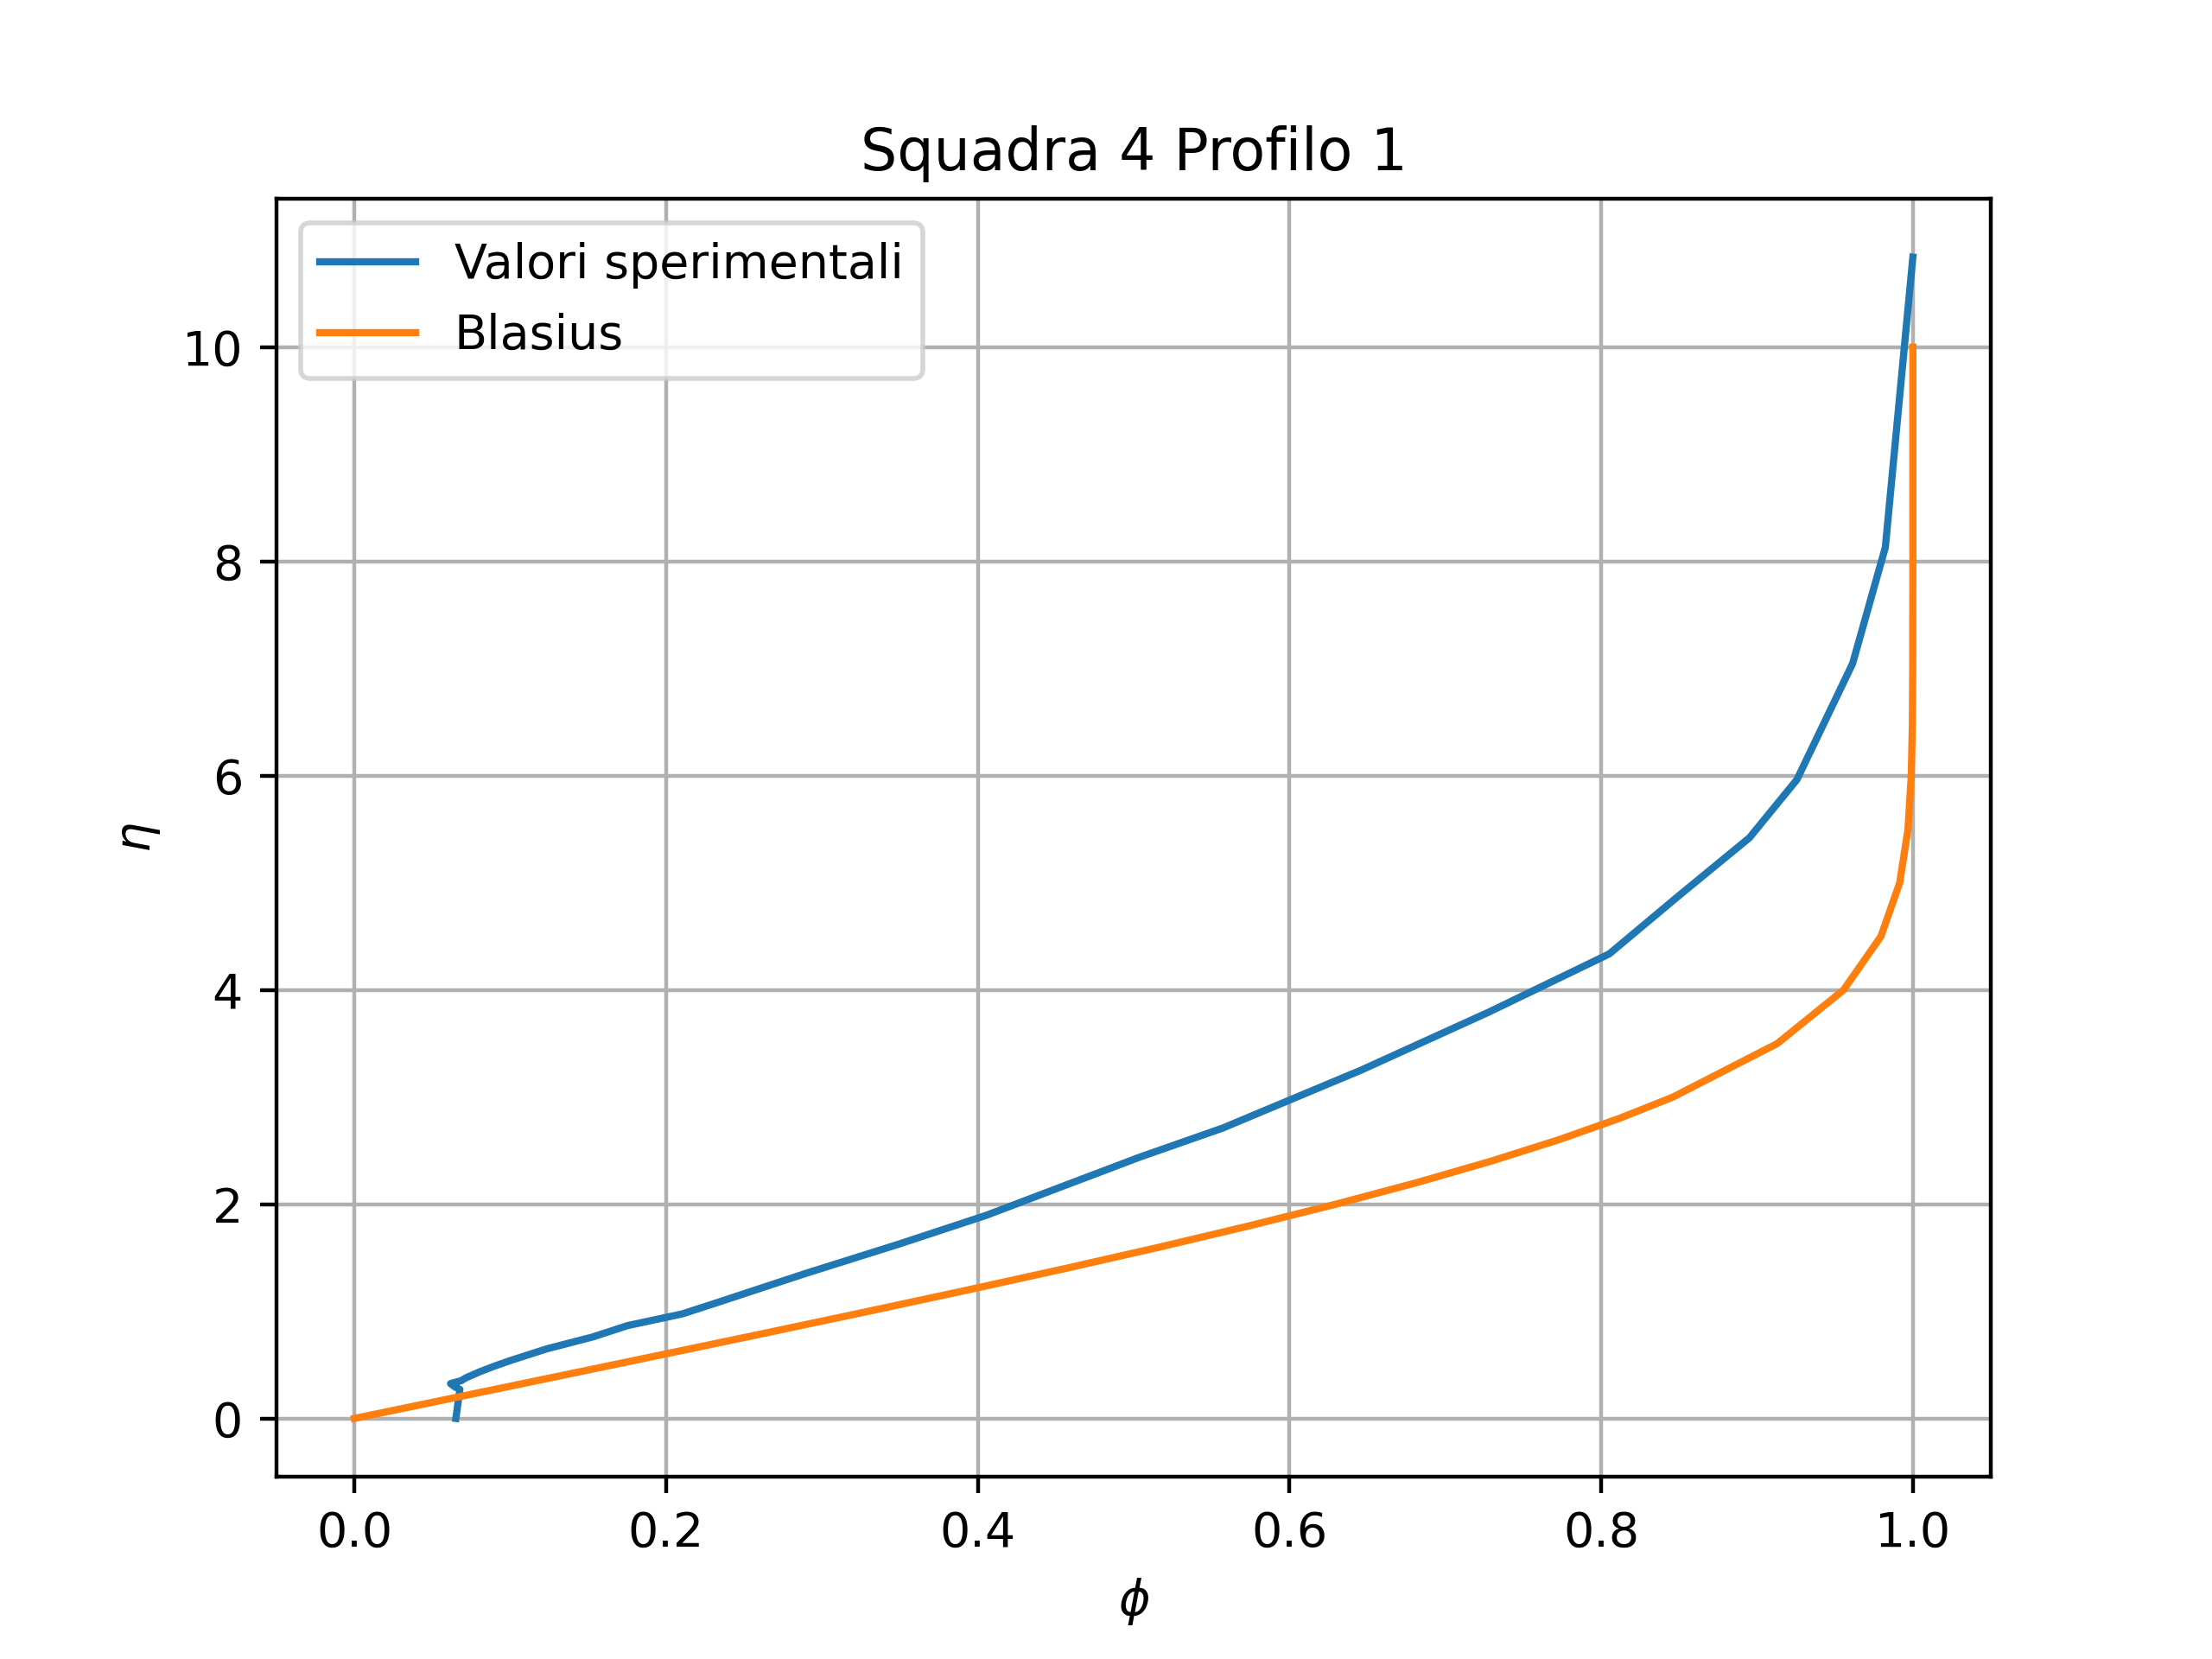
\includegraphics[width=.49\textwidth]{images/9/sq4p1_blasius.png}
    \caption{Confronto con la soluzione di Blasius, squadre 3 e 4}
\end{figure}

\noindent Si osserva come la soluzione di Blasius approssimi bene i valori dei dati sperimentali, seppur non perfettamente. La discrepanza è dovuta al fatto che nonostante il numero di Reynolds locale $Re_x$ sia inferiore al numero di Reynolds critico $Re_{cr}$, lo strato limite non sia completamente laminare bensì transizionale, e presenti quindi fenomeni di turbolenza intermittente.\\\\
L'andamento spurio che si evidenzia nei dati sperimentali per la seconda squadra è dovuto ad un'interferenza con il sostegno della sonda a filo caldo durante l'acquisizione dei dati.

\subsubsection{Strato limite turbolento}
Nel caso di strato limite turbolento, è opportuno considerare le variabili interne dello strato limite $u^+$ e $y^+$, dove:
\begin{equation*}
    y^+ = \frac{y u_\tau}{\nu} \qquad u^+ = \frac{u}{u_\tau} \qquad u_\tau = \sqrt{\frac{\tau_w}{\rho}} = U_e \sqrt{\frac{c_f}2}
\end{equation*}
Per ricavare il coefficiente di sforzo di attrito a parete $c_f$ si utilizza il metodo di Clauser, che ricorre alla legge logaritmica di parete:
\begin{equation*}
    \frac{u}{u_\tau} = \frac 1k \ln \frac{y u_\tau}{\nu} + C
\end{equation*}
Se si moltiplica e divide per la velocità esterna $U_e$, si ottiene:
\begin{equation*}
    \frac{u}{U_e} = \frac{u_\tau}{U_e}\left[ \frac 1k \ln\left( \frac{yU_e}{\nu}\frac{u_\tau}{U_e} \right) +C\right] = \sqrt{\frac{c_f}2}\left[ \frac 1k \ln\left( \frac{yU_e}{\nu}\sqrt{\frac{c_f}2} \right) +C\right]
\end{equation*}
Il metodo prevede di diagrammare i dati in forma semilogaritmica. In ascisse si riporta $yU_e/\nu$ con asse logaritmico e in ordinate si riporta la velocità adimensionale $u/U_e$ con asse lineare. Si tracciano quindi delle curve parametriche corrispondenti ai profili di velocità al variare del coefficiente di sforzo di attrito a parete $c_f$.
\newpage
\noindent In questo modo si costruisce la mappa di Clauser:
\begin{figure}[H]
    \centering
    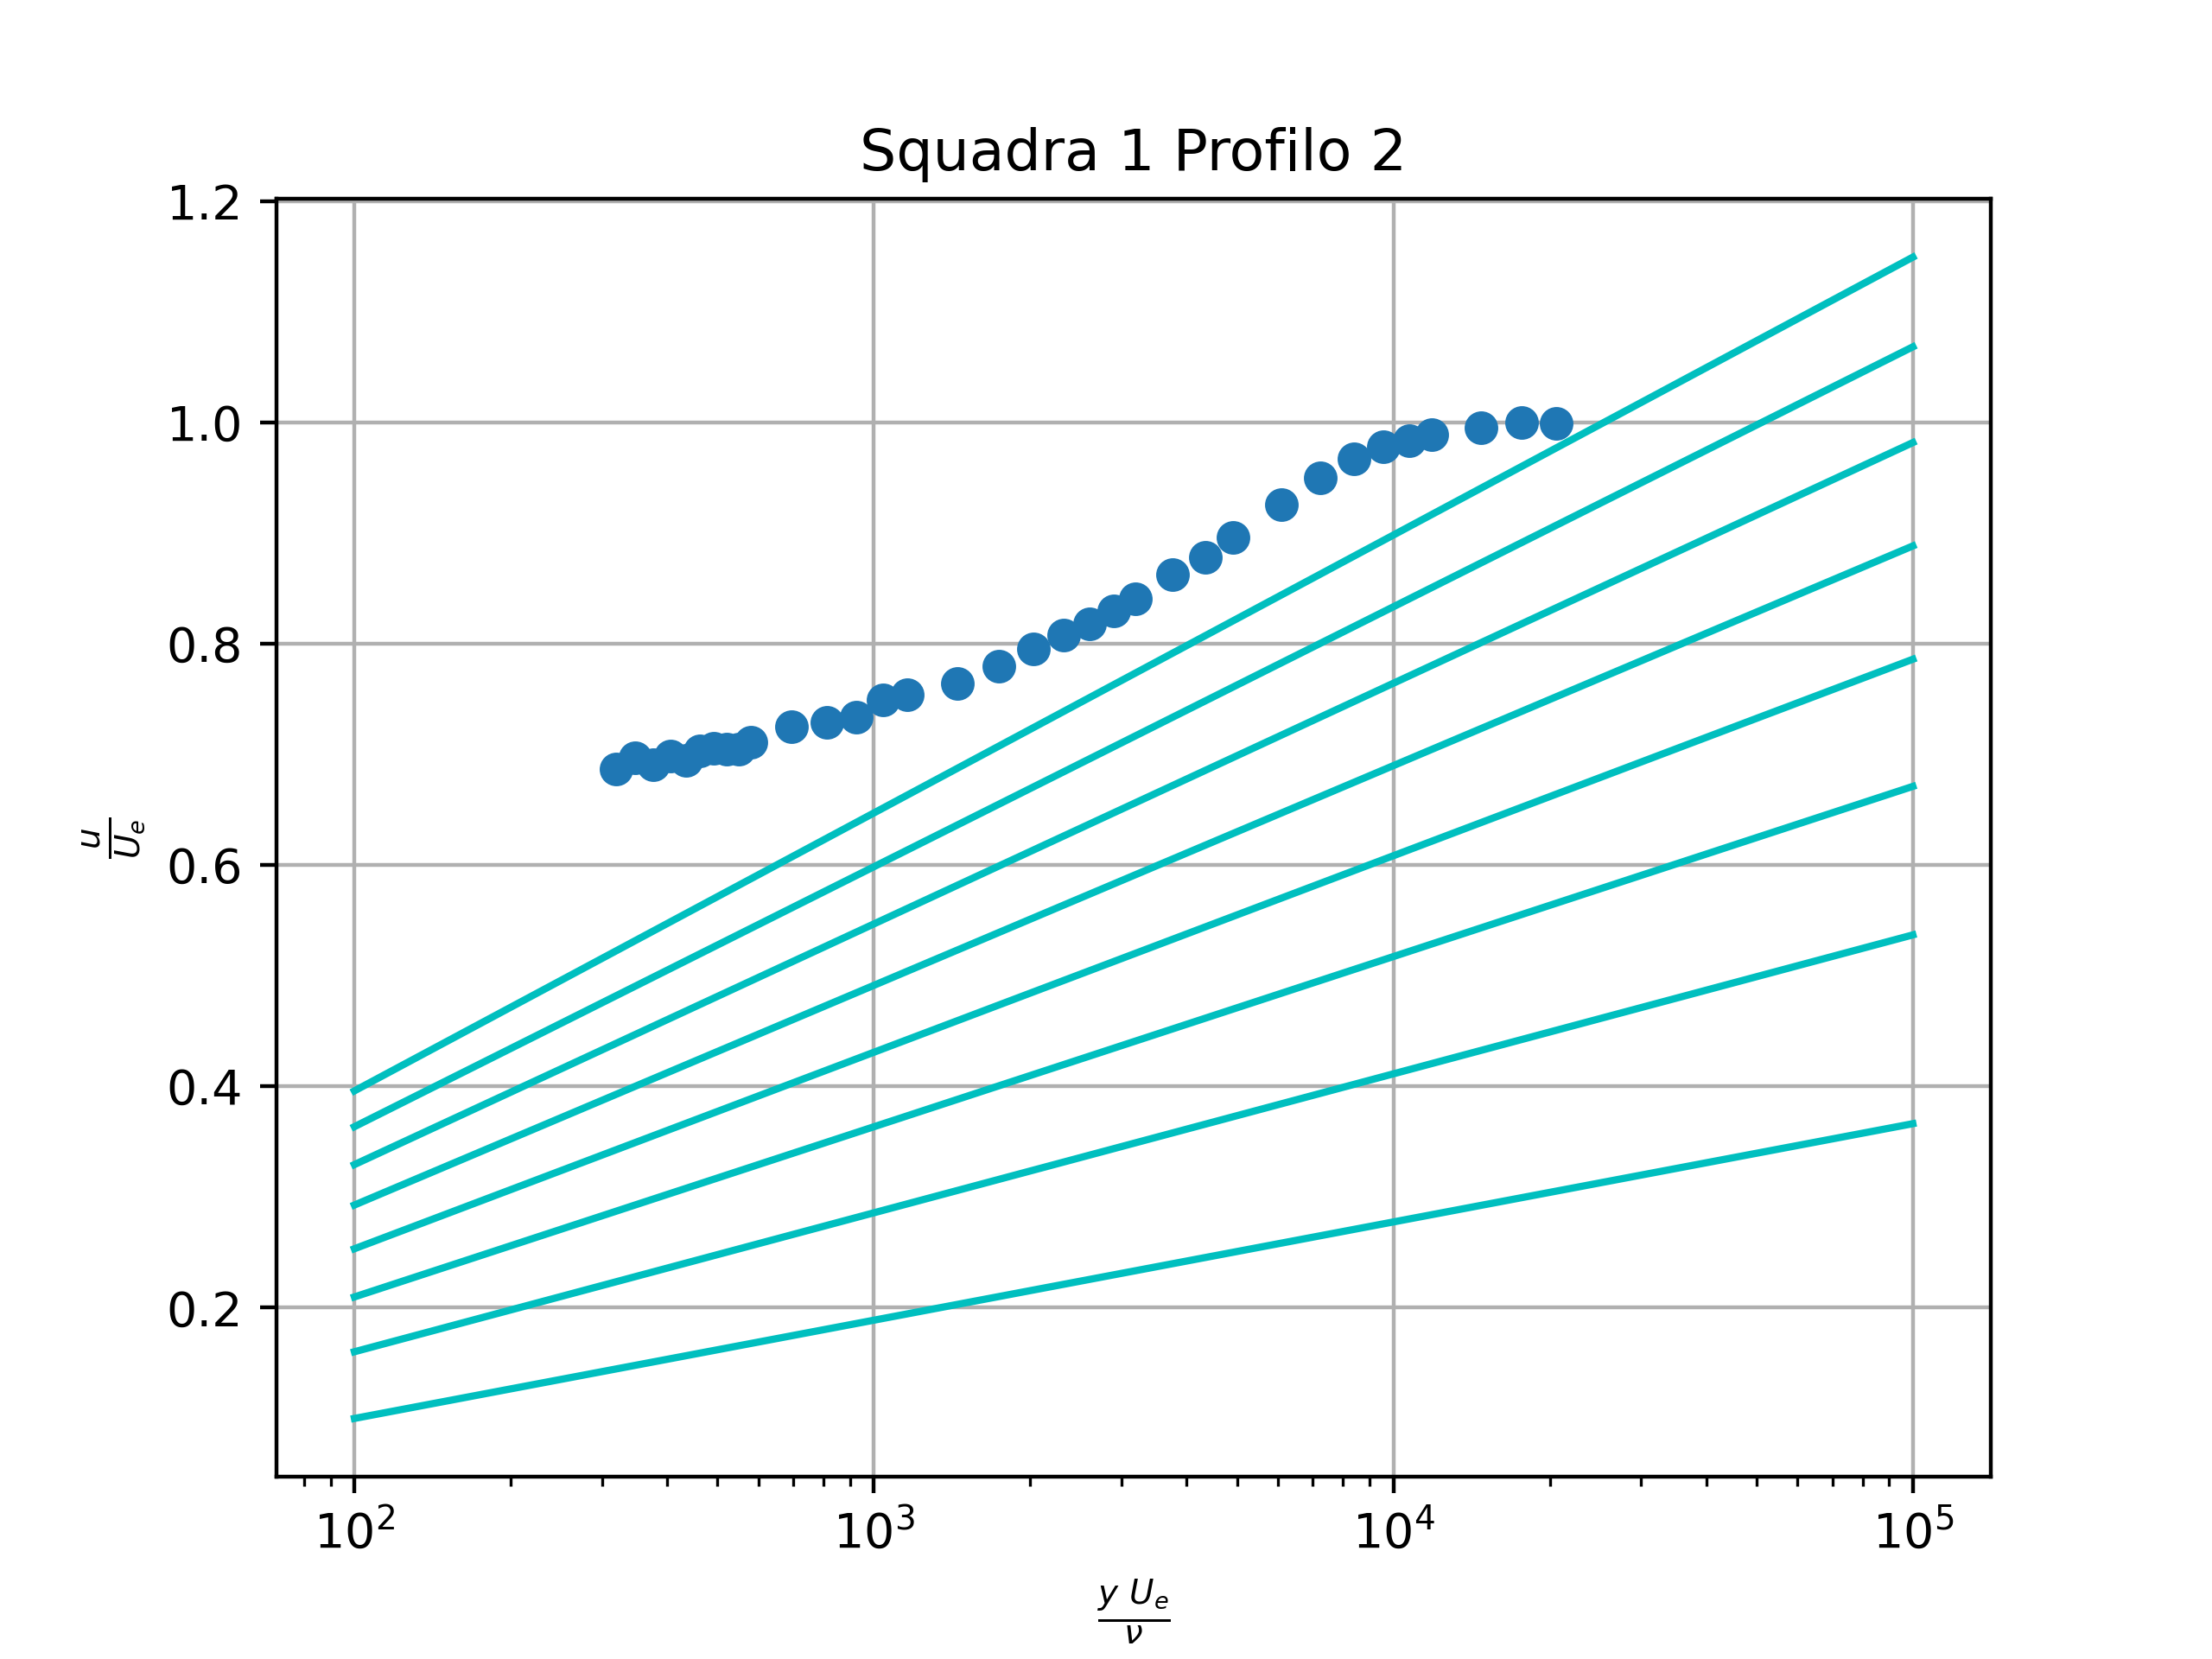
\includegraphics[width=.8\textwidth]{images/9/sq1p2clauser.png}
    \caption{Mappa di Clauser per il profilo turbolento della prima squadra}
\end{figure}

\begin{figure}[H]
    \centering
    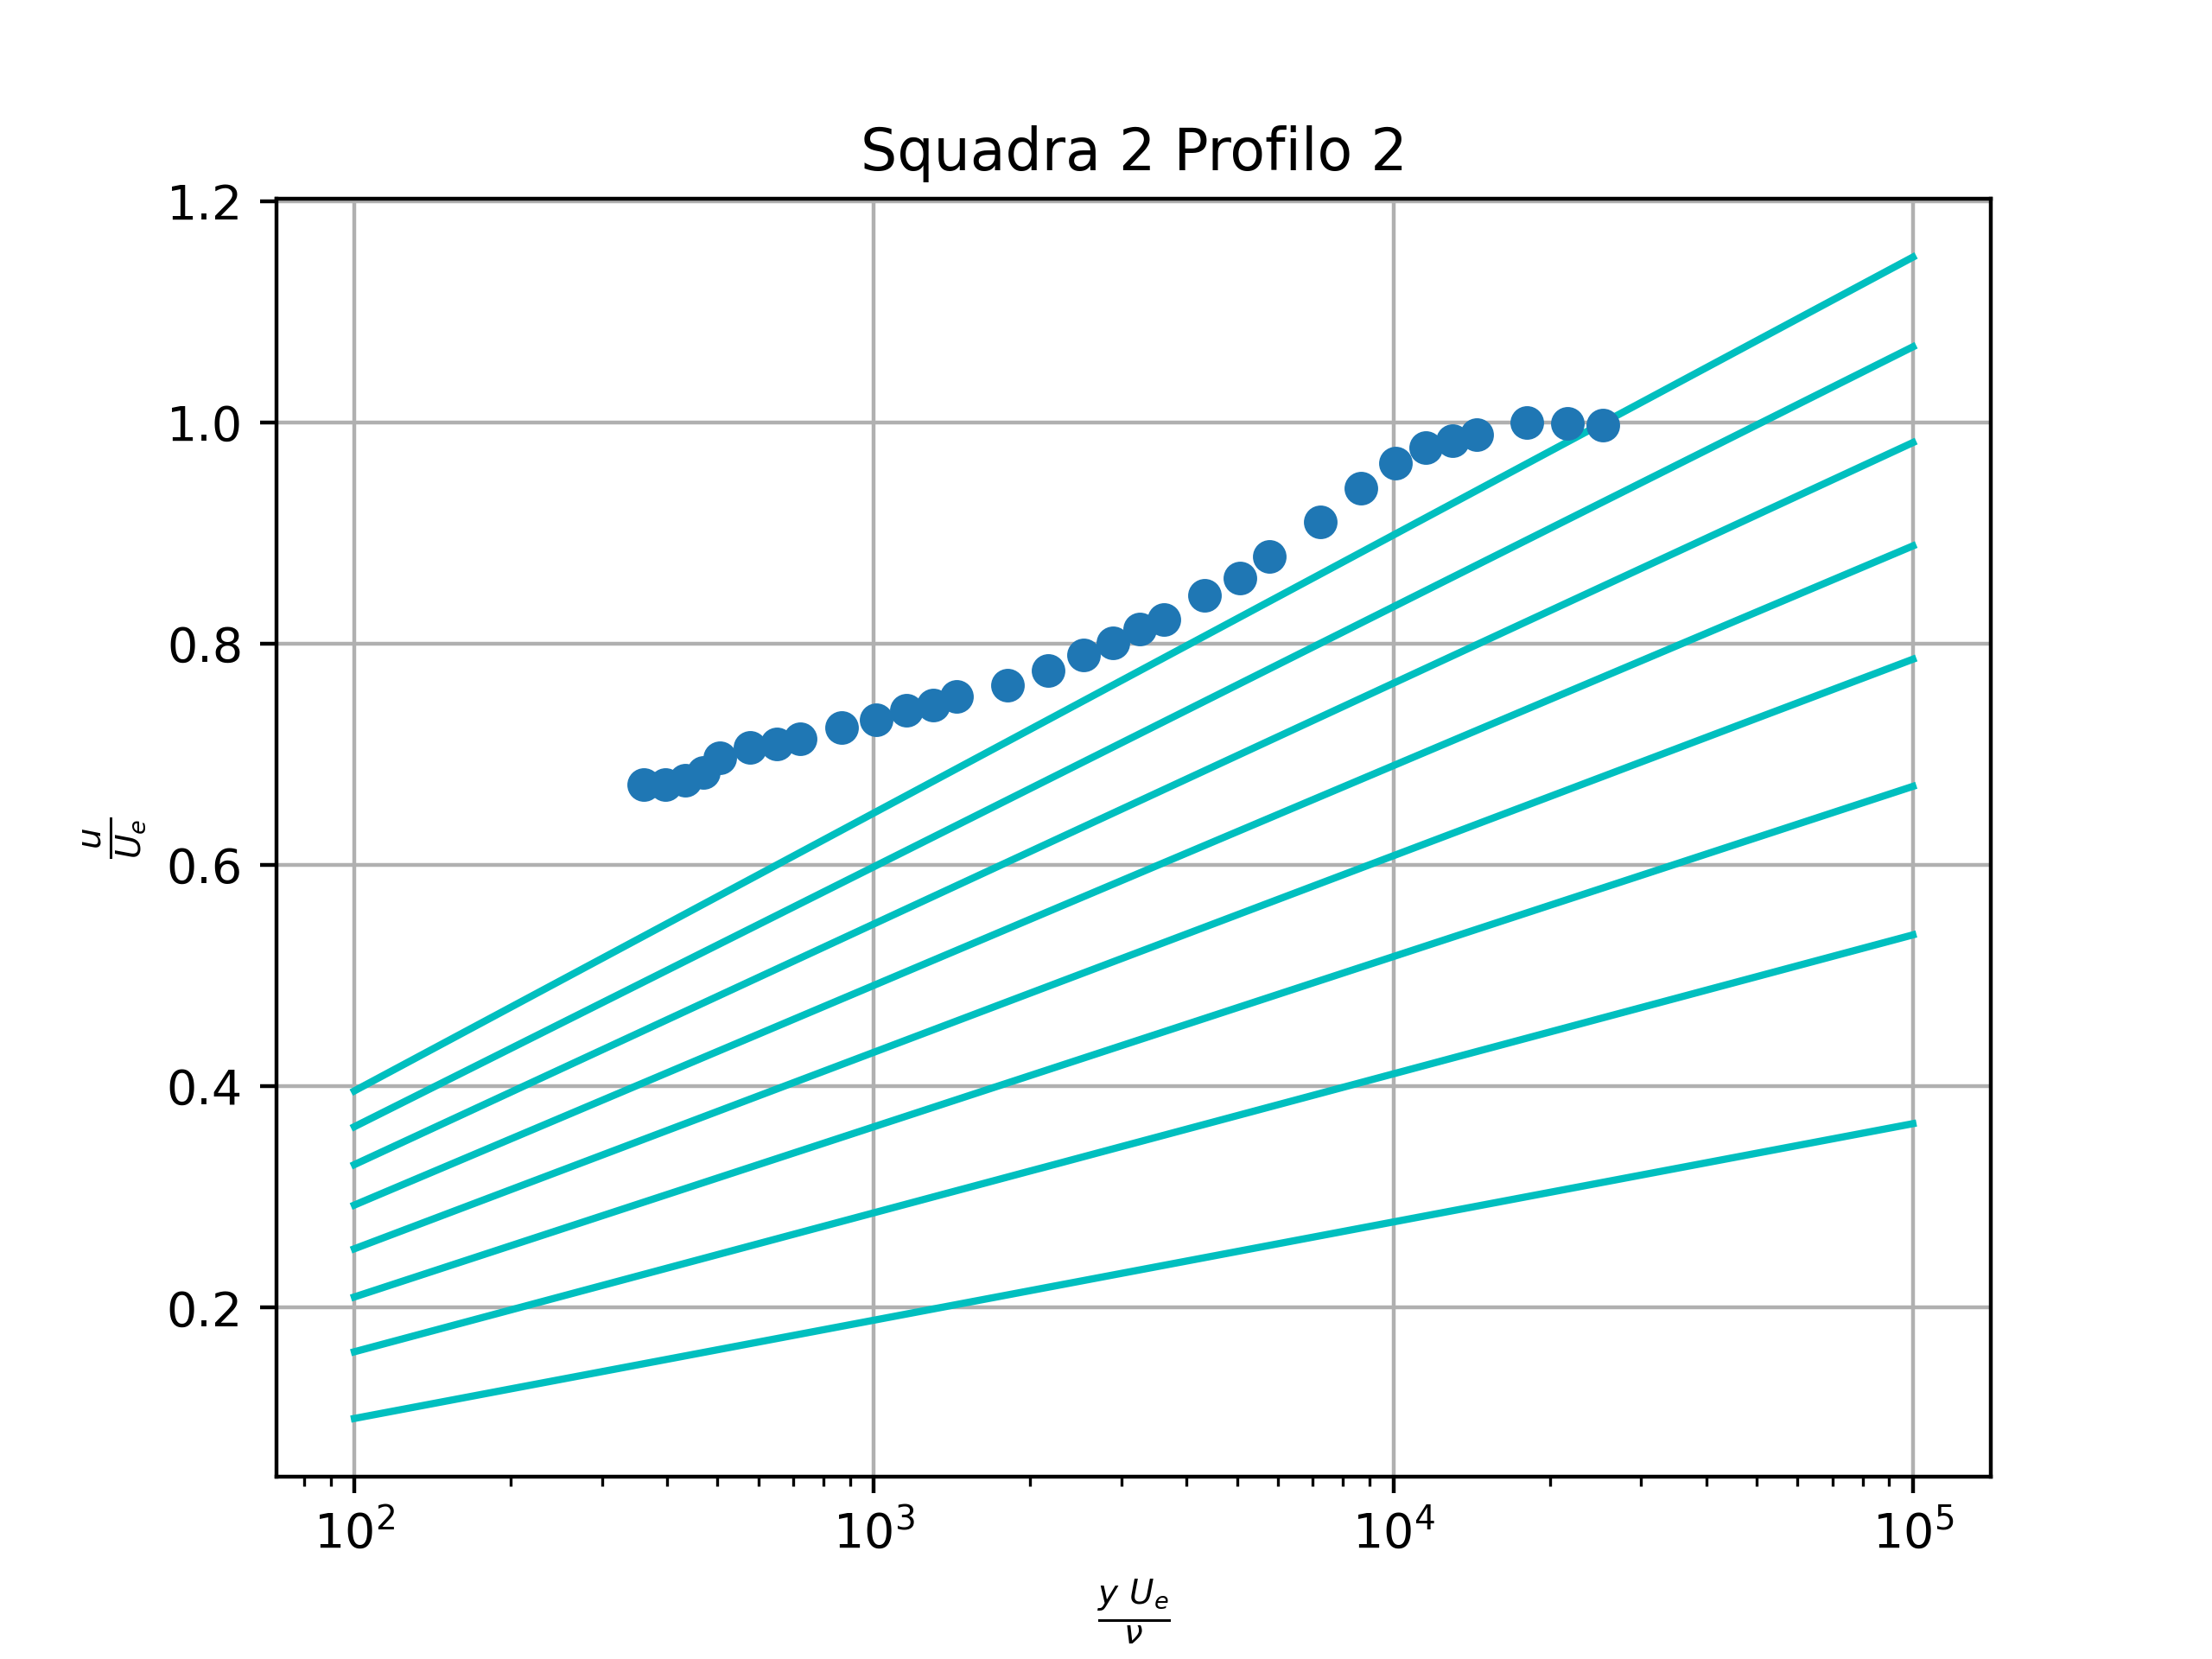
\includegraphics[width=.8\textwidth]{images/9/sq2p2clauser.png}
    \caption{Mappa di Clauser per il profilo turbolento della seconda squadra}
\end{figure}

\begin{figure}[H]
    \centering
    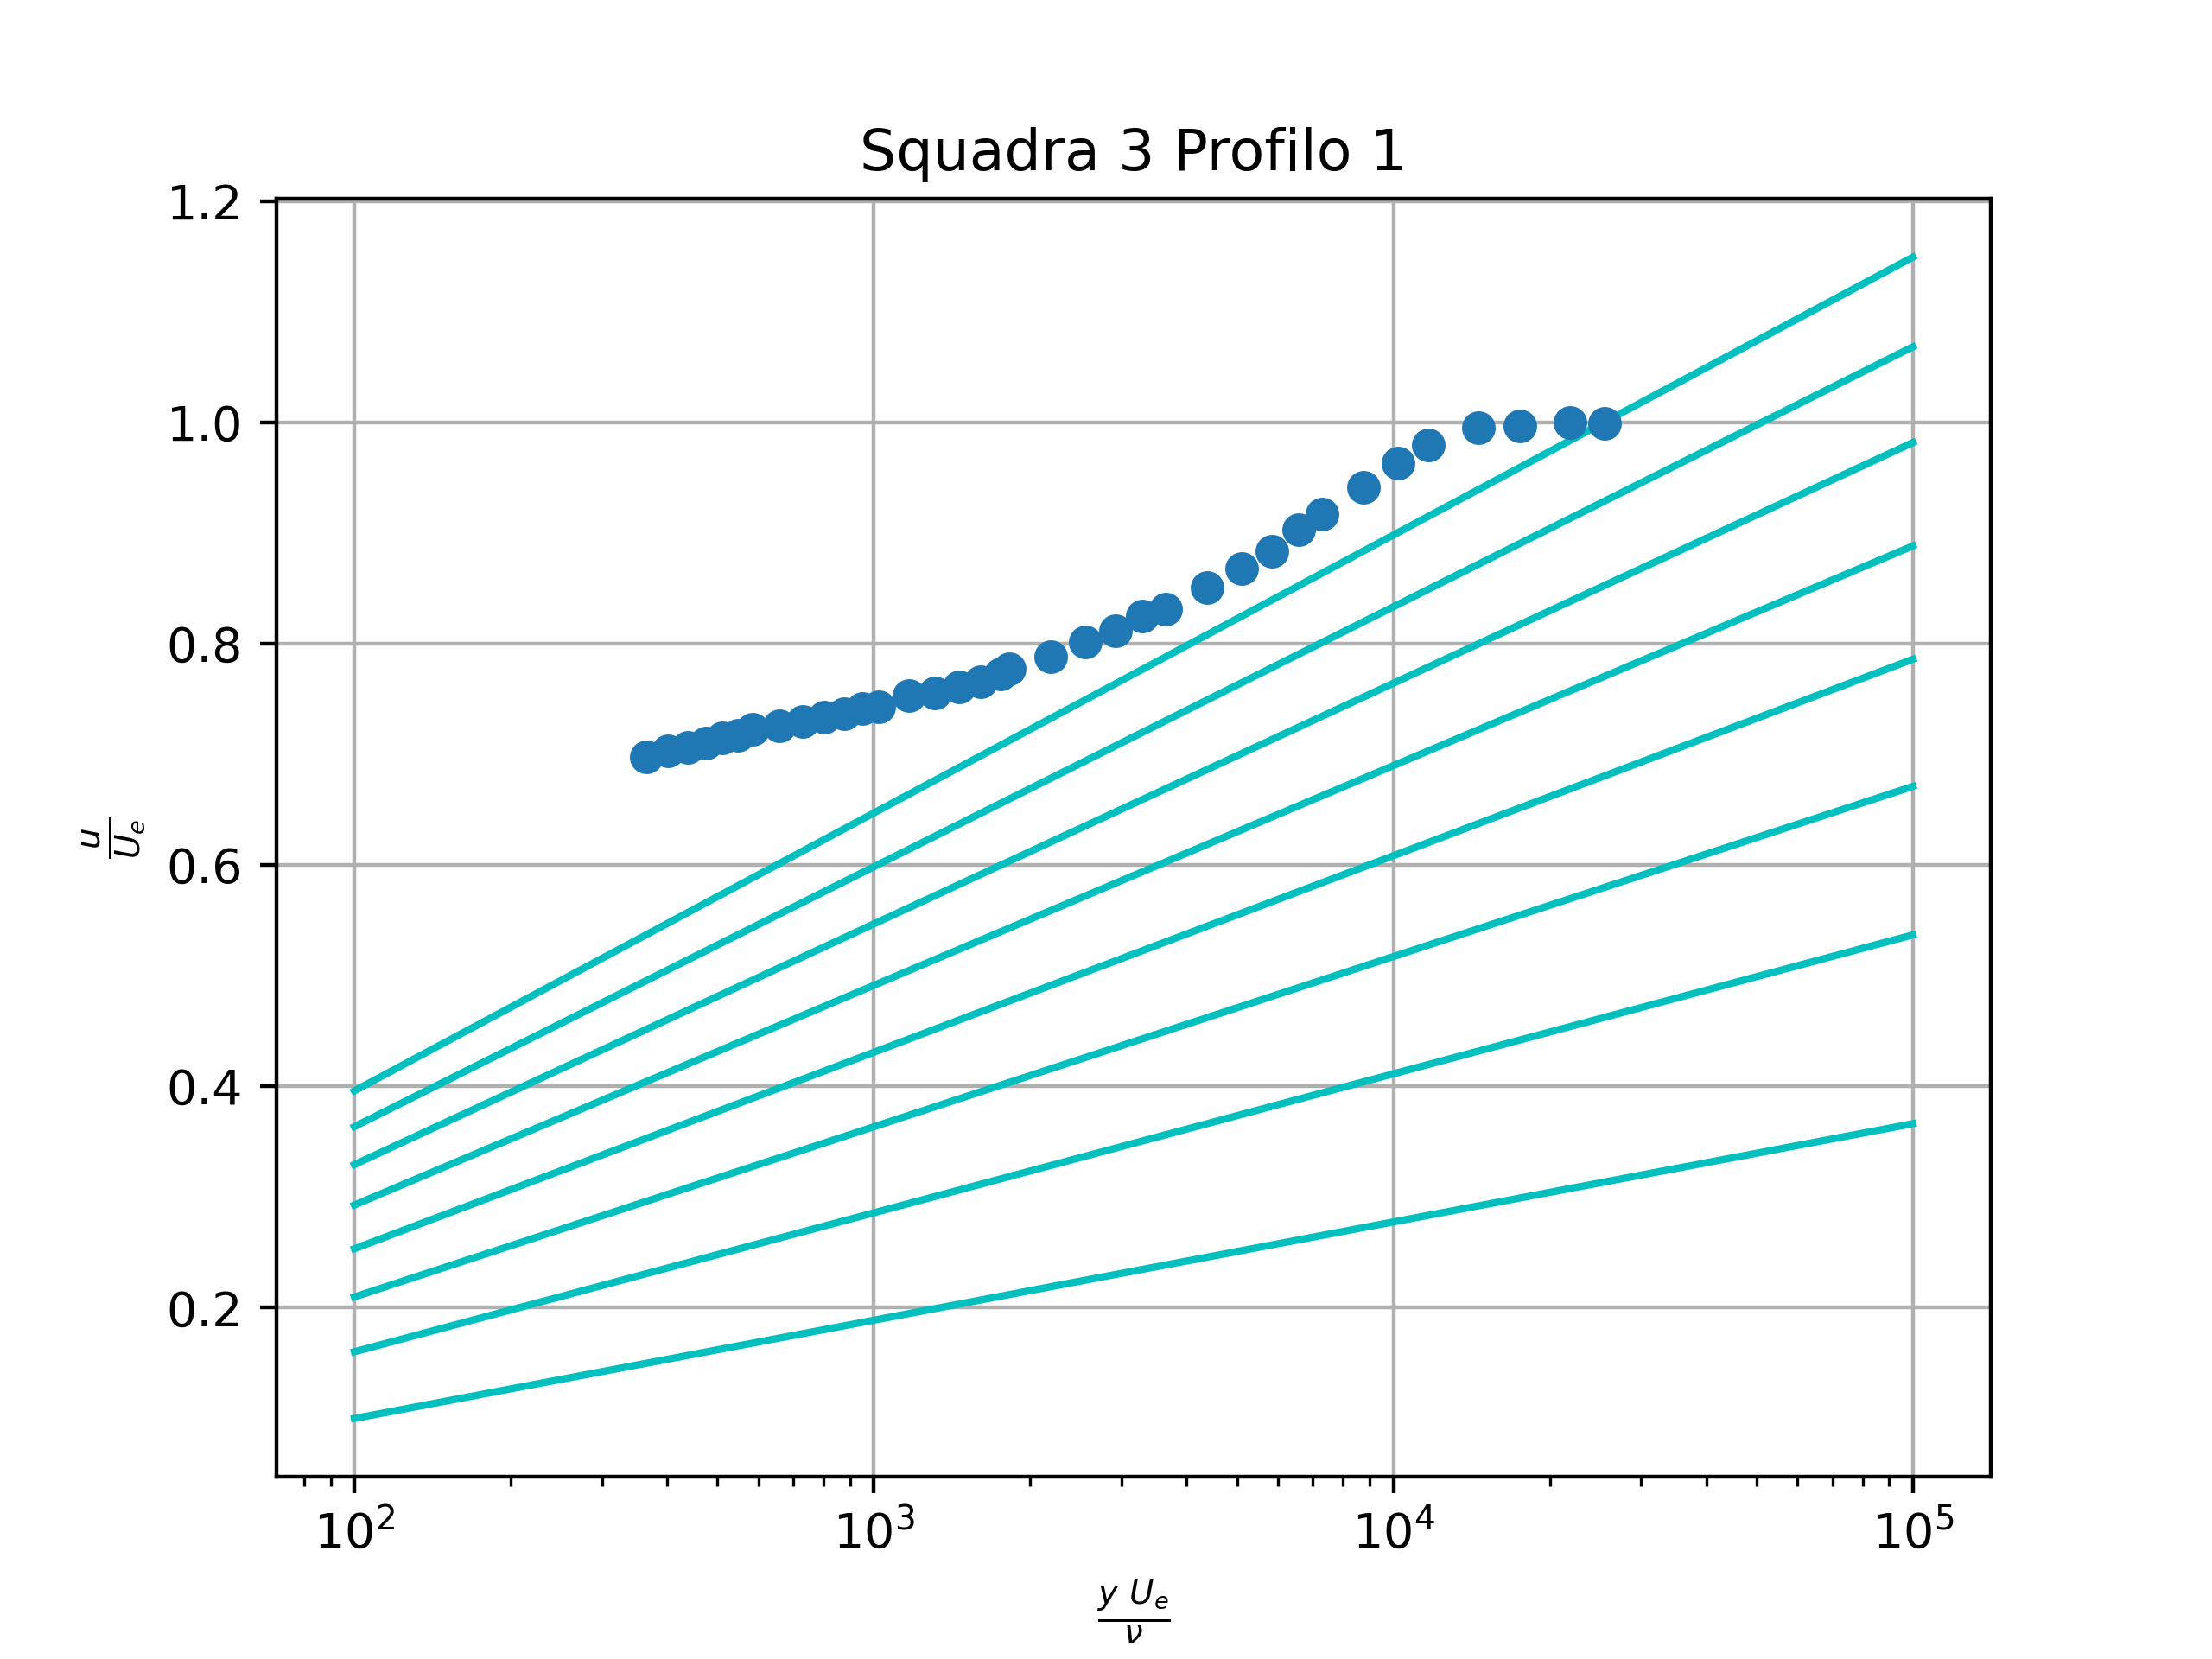
\includegraphics[width=.8\textwidth]{images/9/sq3p1clauser.png}
    \caption{Mappa di Clauser per il profilo turbolento della terza squadra}
\end{figure}

\begin{figure}[H]
    \centering
    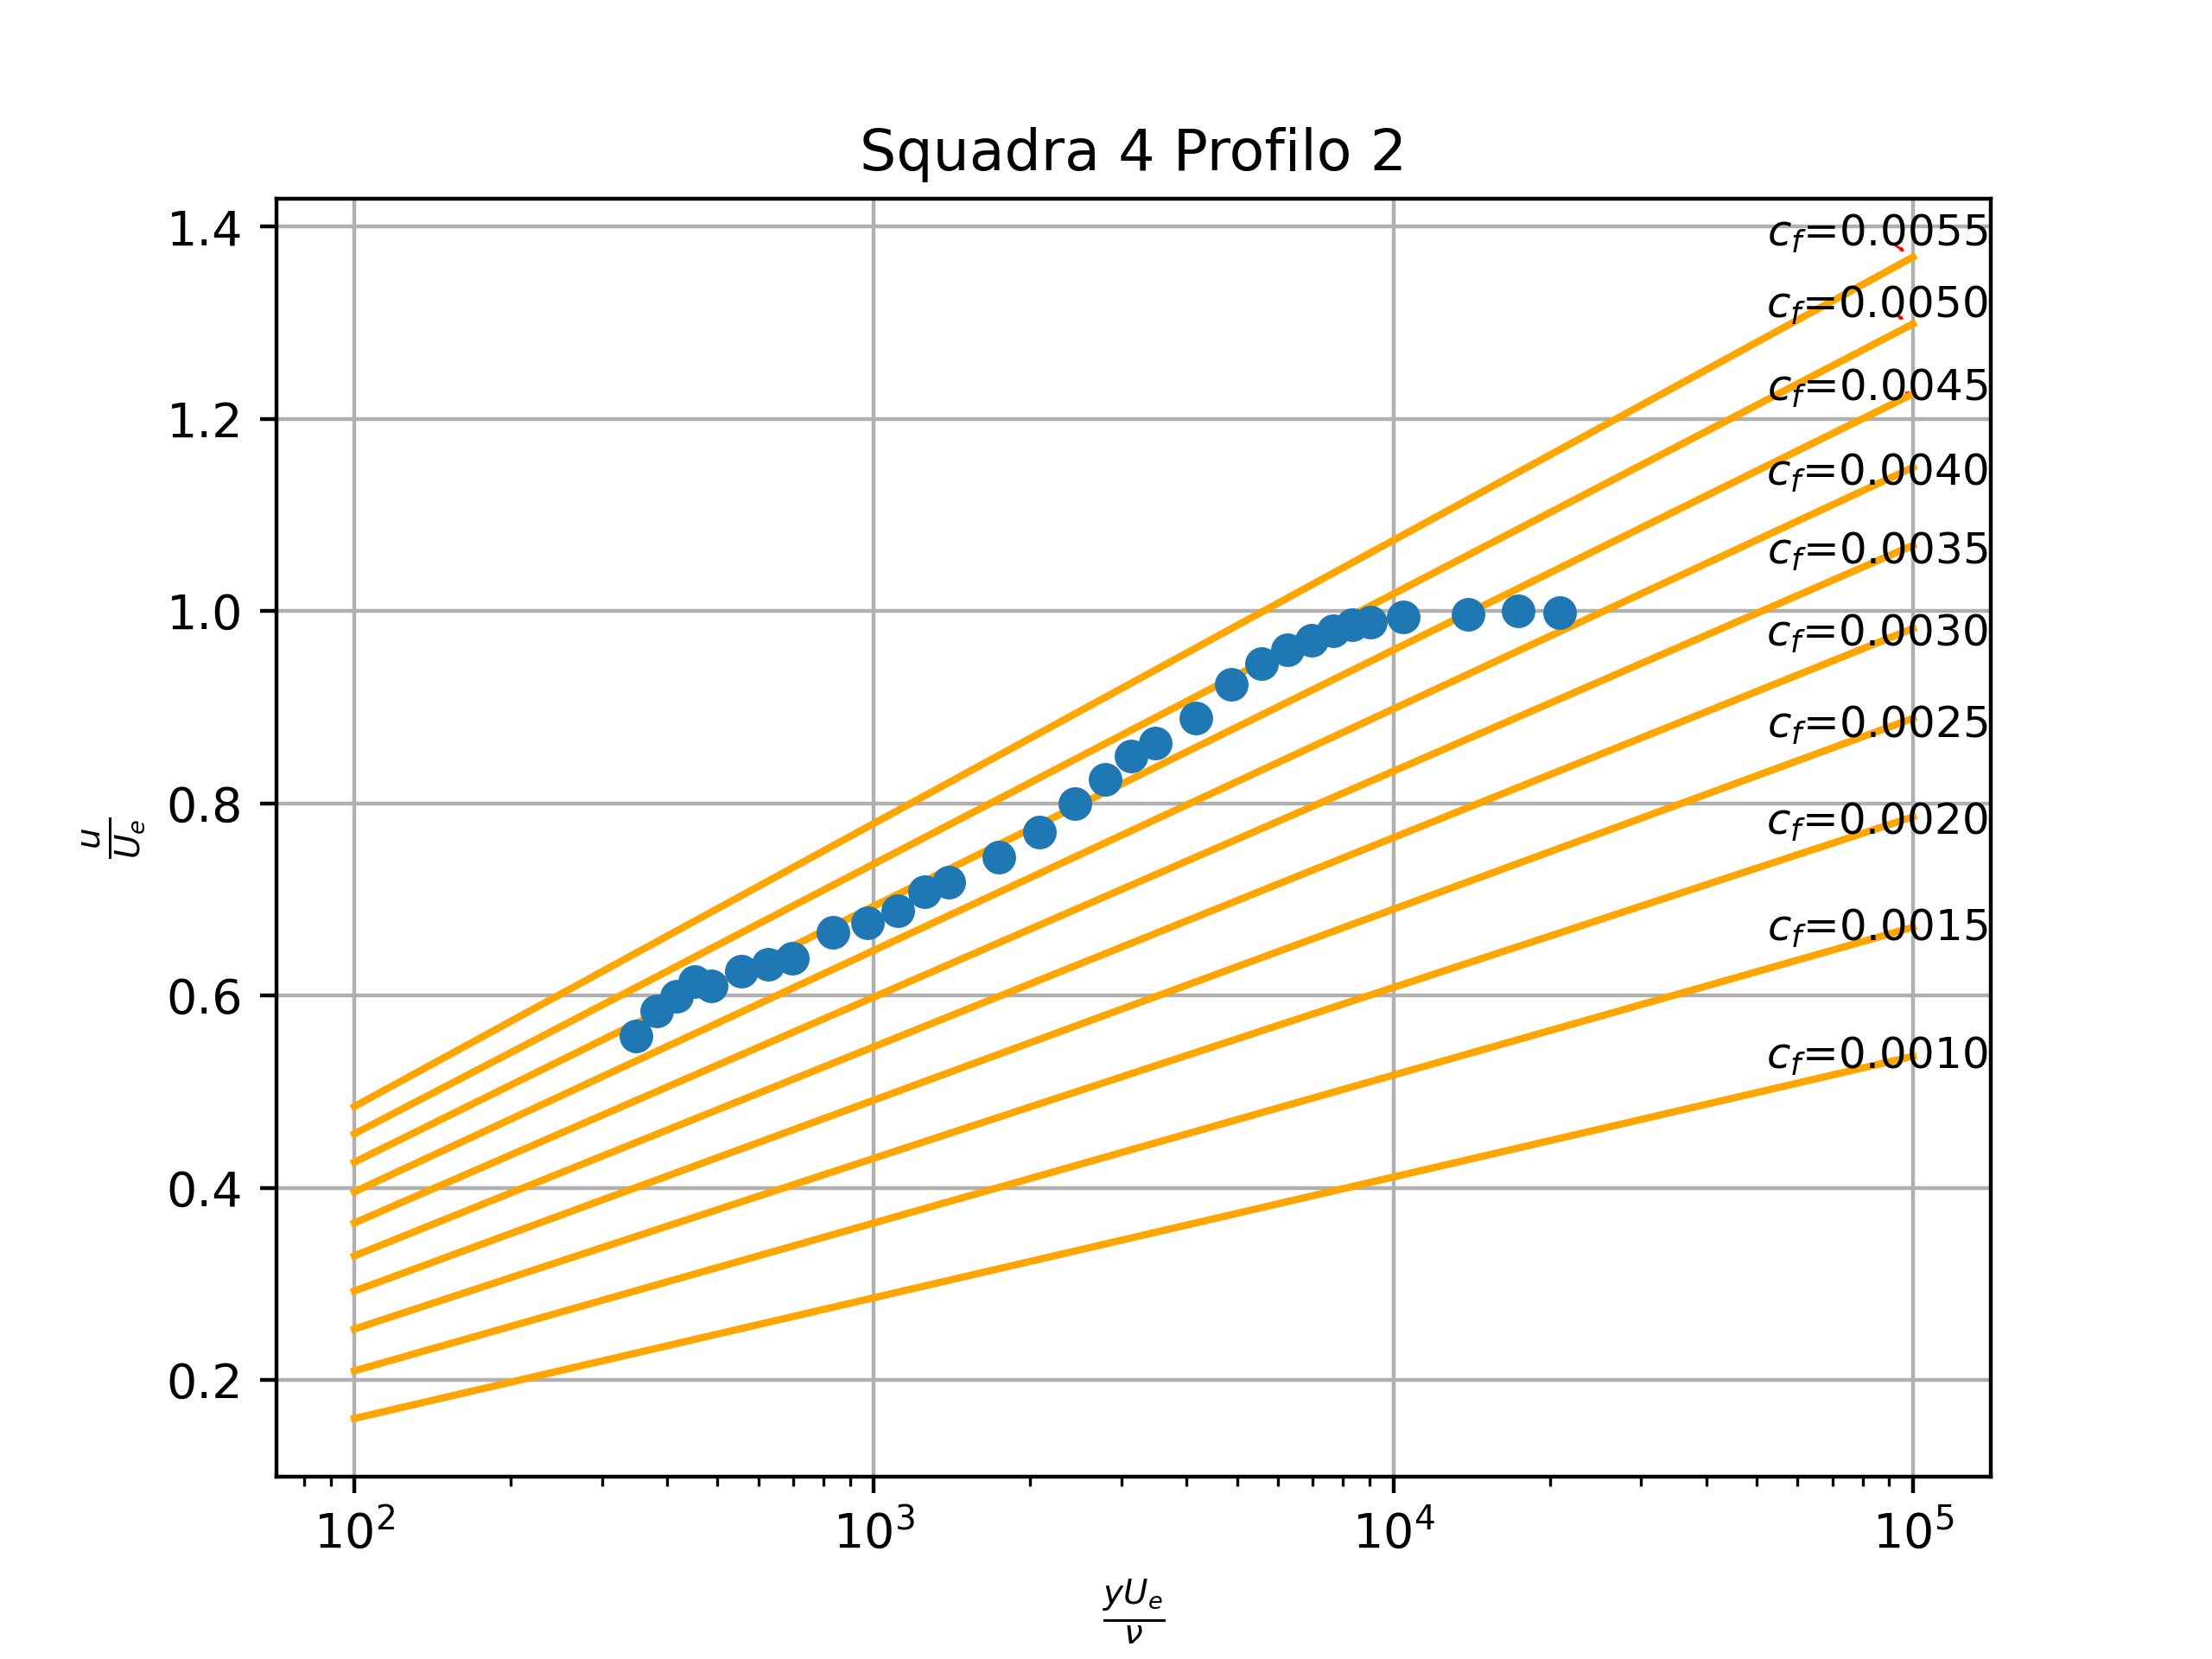
\includegraphics[width=.8\textwidth]{images/9/sq4p2clauser.png}
    \caption{Mappa di Clauser per il profilo turbolento della quarta squadra}
\end{figure}

\newpage
\noindent Dalle mappe di Clauser ottenute è possibile ricavare il coefficiente di sforzo di attrito a parete $c_f$, quindi lo sforzo di attrito a parete $\tau_w$ e la velocità di attrito $u_\tau$, secondo le relazioni:
\begin{equation*}
    \tau_ w = \frac12 \rho U_e^2 c_f \qquad u_\tau = \sqrt{\frac{\tau_w}\rho}=U_e\sqrt{\frac{c_f}2}
\end{equation*}
Per le quattro squadre si ottiene:\\
Squadra 1: $c_f = 0.00474\ \rightarrow\ \tau_w = 0.22\,N/m^2$\\
Squadra 2: $c_f = 0.00447\ \rightarrow\ \tau_w = 0.32\,N/m^2$\\
Squadra 3: $c_f = 0.00454\ \rightarrow\ \tau_w = 0.33\,N/m^2$\\
Squadra 4: $c_f = 0.00453\ \rightarrow\ \tau_w = 0.31\,N/m^2$\\\\
I risultati sperimentali rispettano le leggi empiriche precedentemente enunciate.\\\\
Una volta ricavata la velocità di attrito, è possibile calcolare le grandezze interne dello strato limite turbolento $u^+$ e $y^+$.\\\\
Si ottengono quindi i seguenti diagrammi per le quattro squadre, dove si evidenzia un asintoto orizzontale per:
\begin{equation*}
    u^+_{asint} = \sqrt{\frac{2}{c_f}} = \frac{U_e}{u_\tau}
\end{equation*}
\begin{figure}[H]
    \centering
    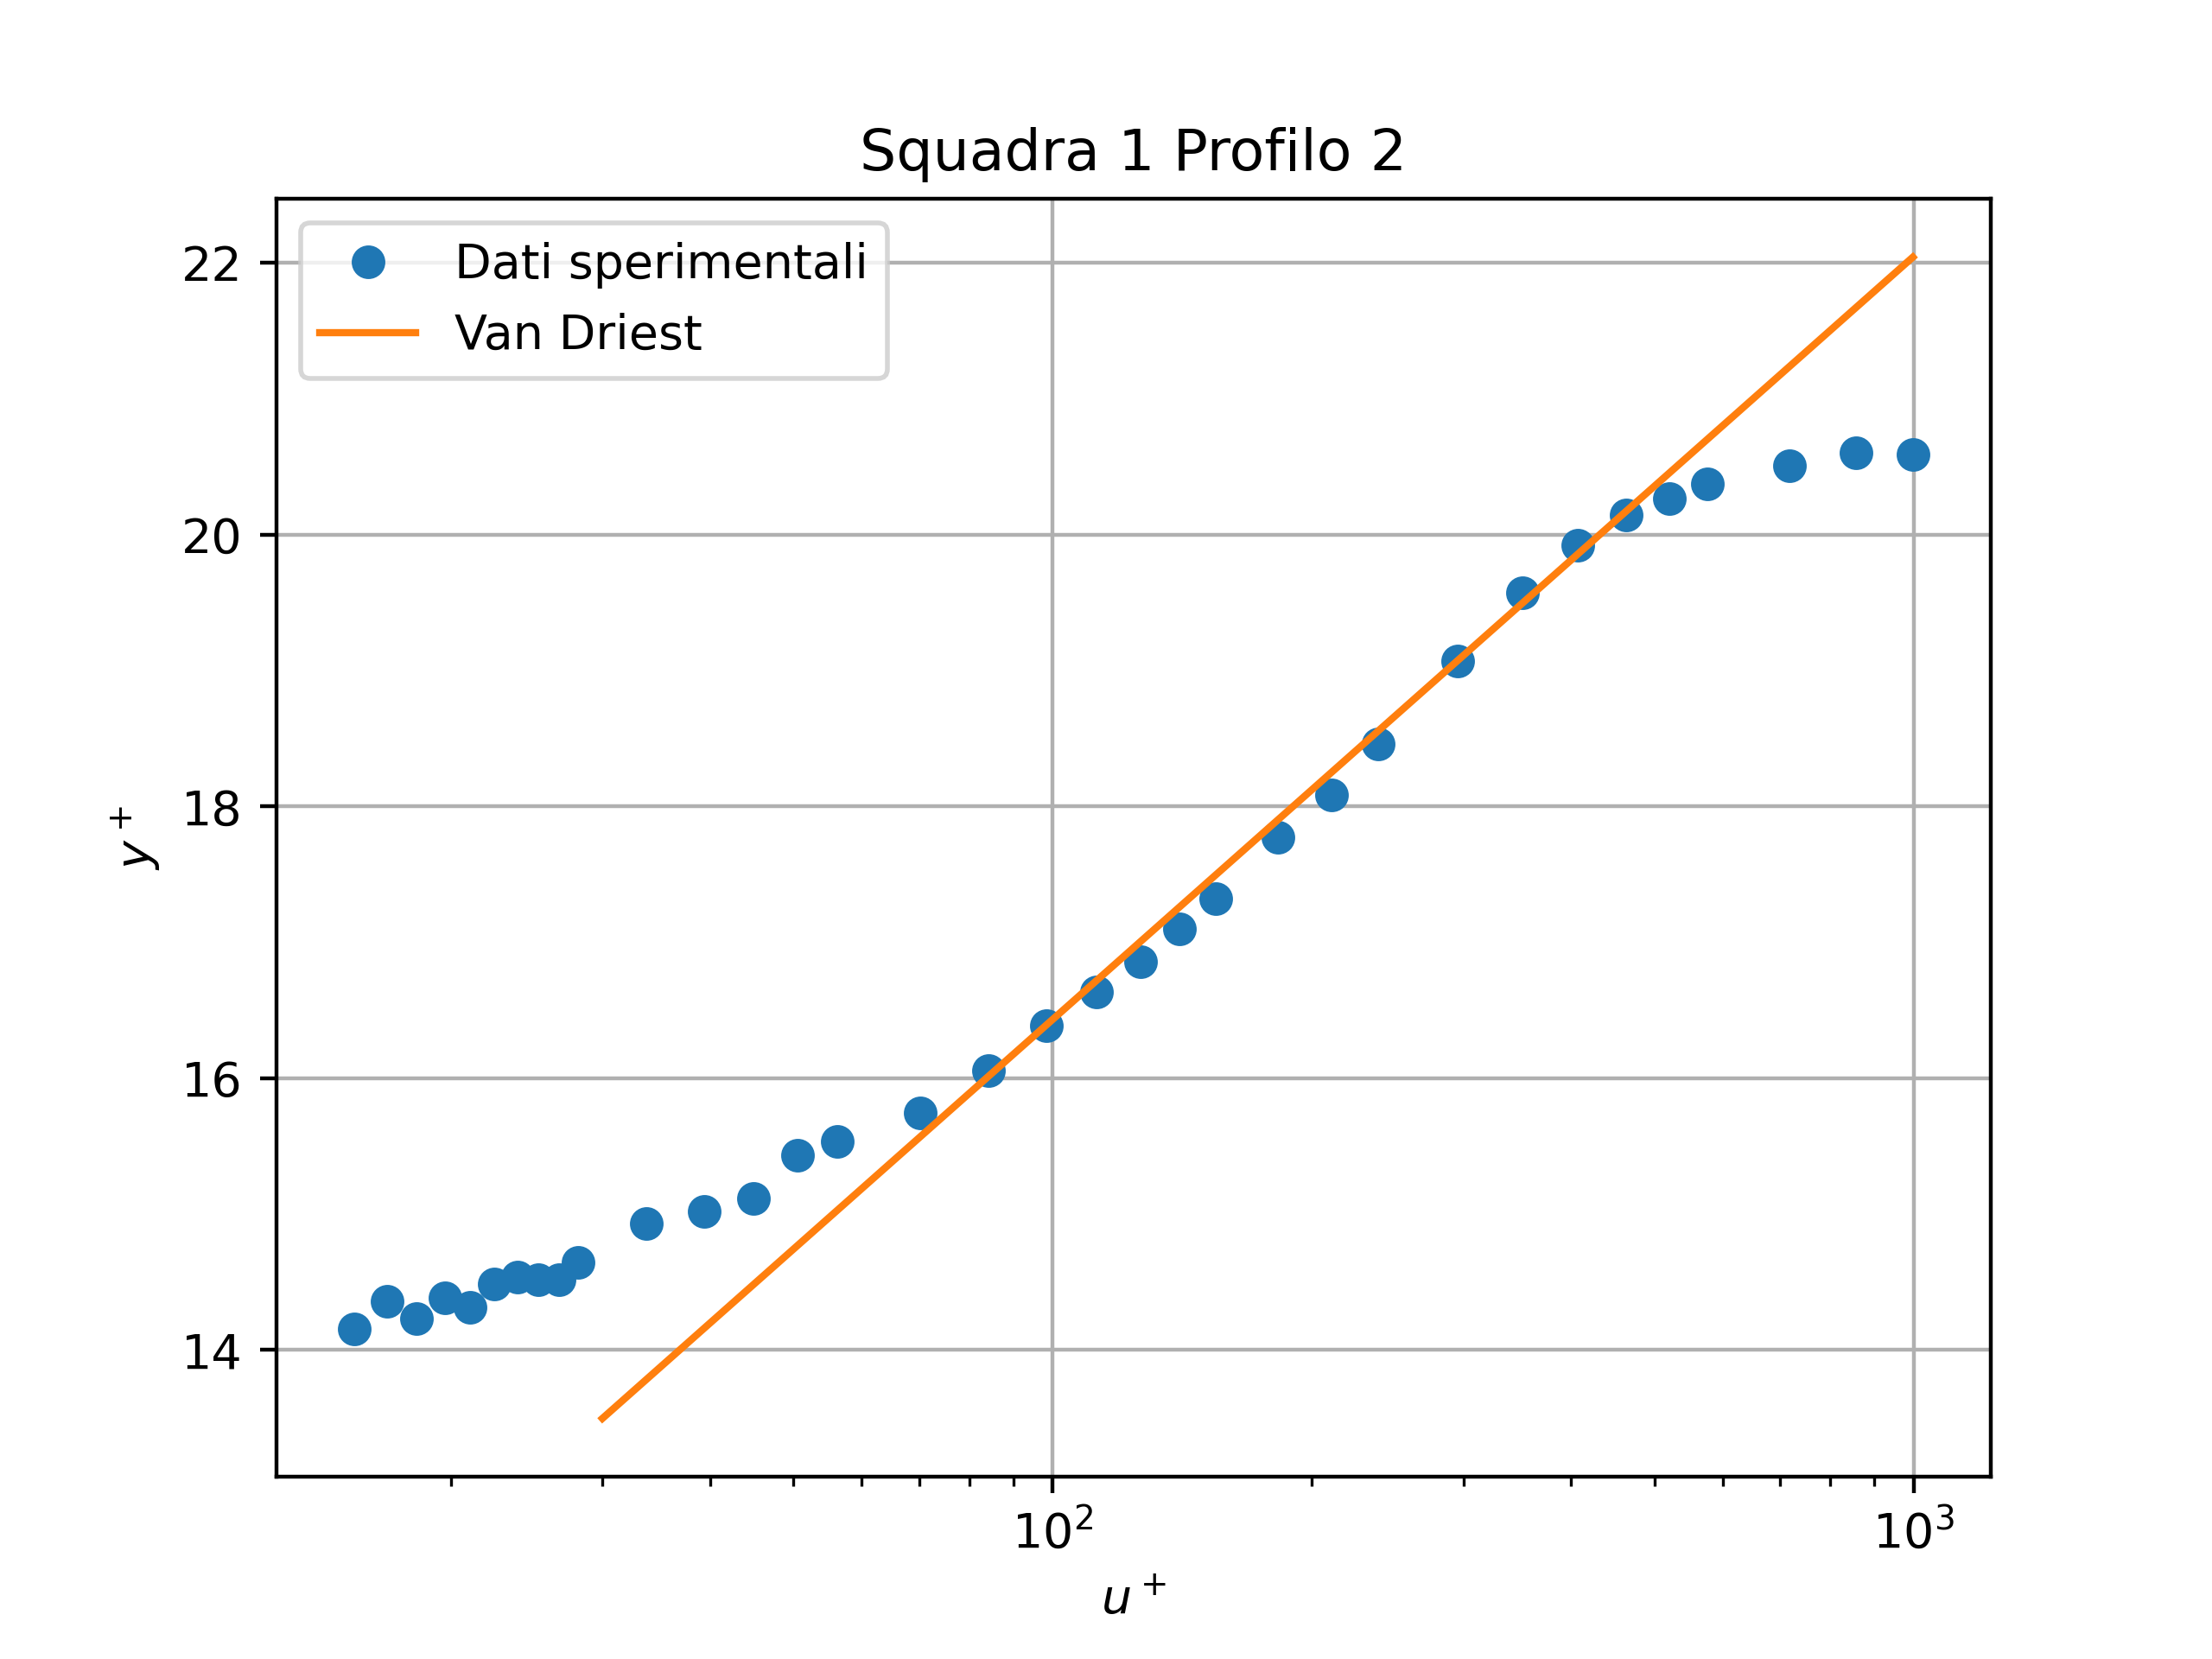
\includegraphics[width=.85\textwidth]{images/9/sq1p2+.png}
    \caption{Diagramma $u^+=f(y^+)$ per la prima squadra}
\end{figure}

\begin{figure}[H]
    \centering
    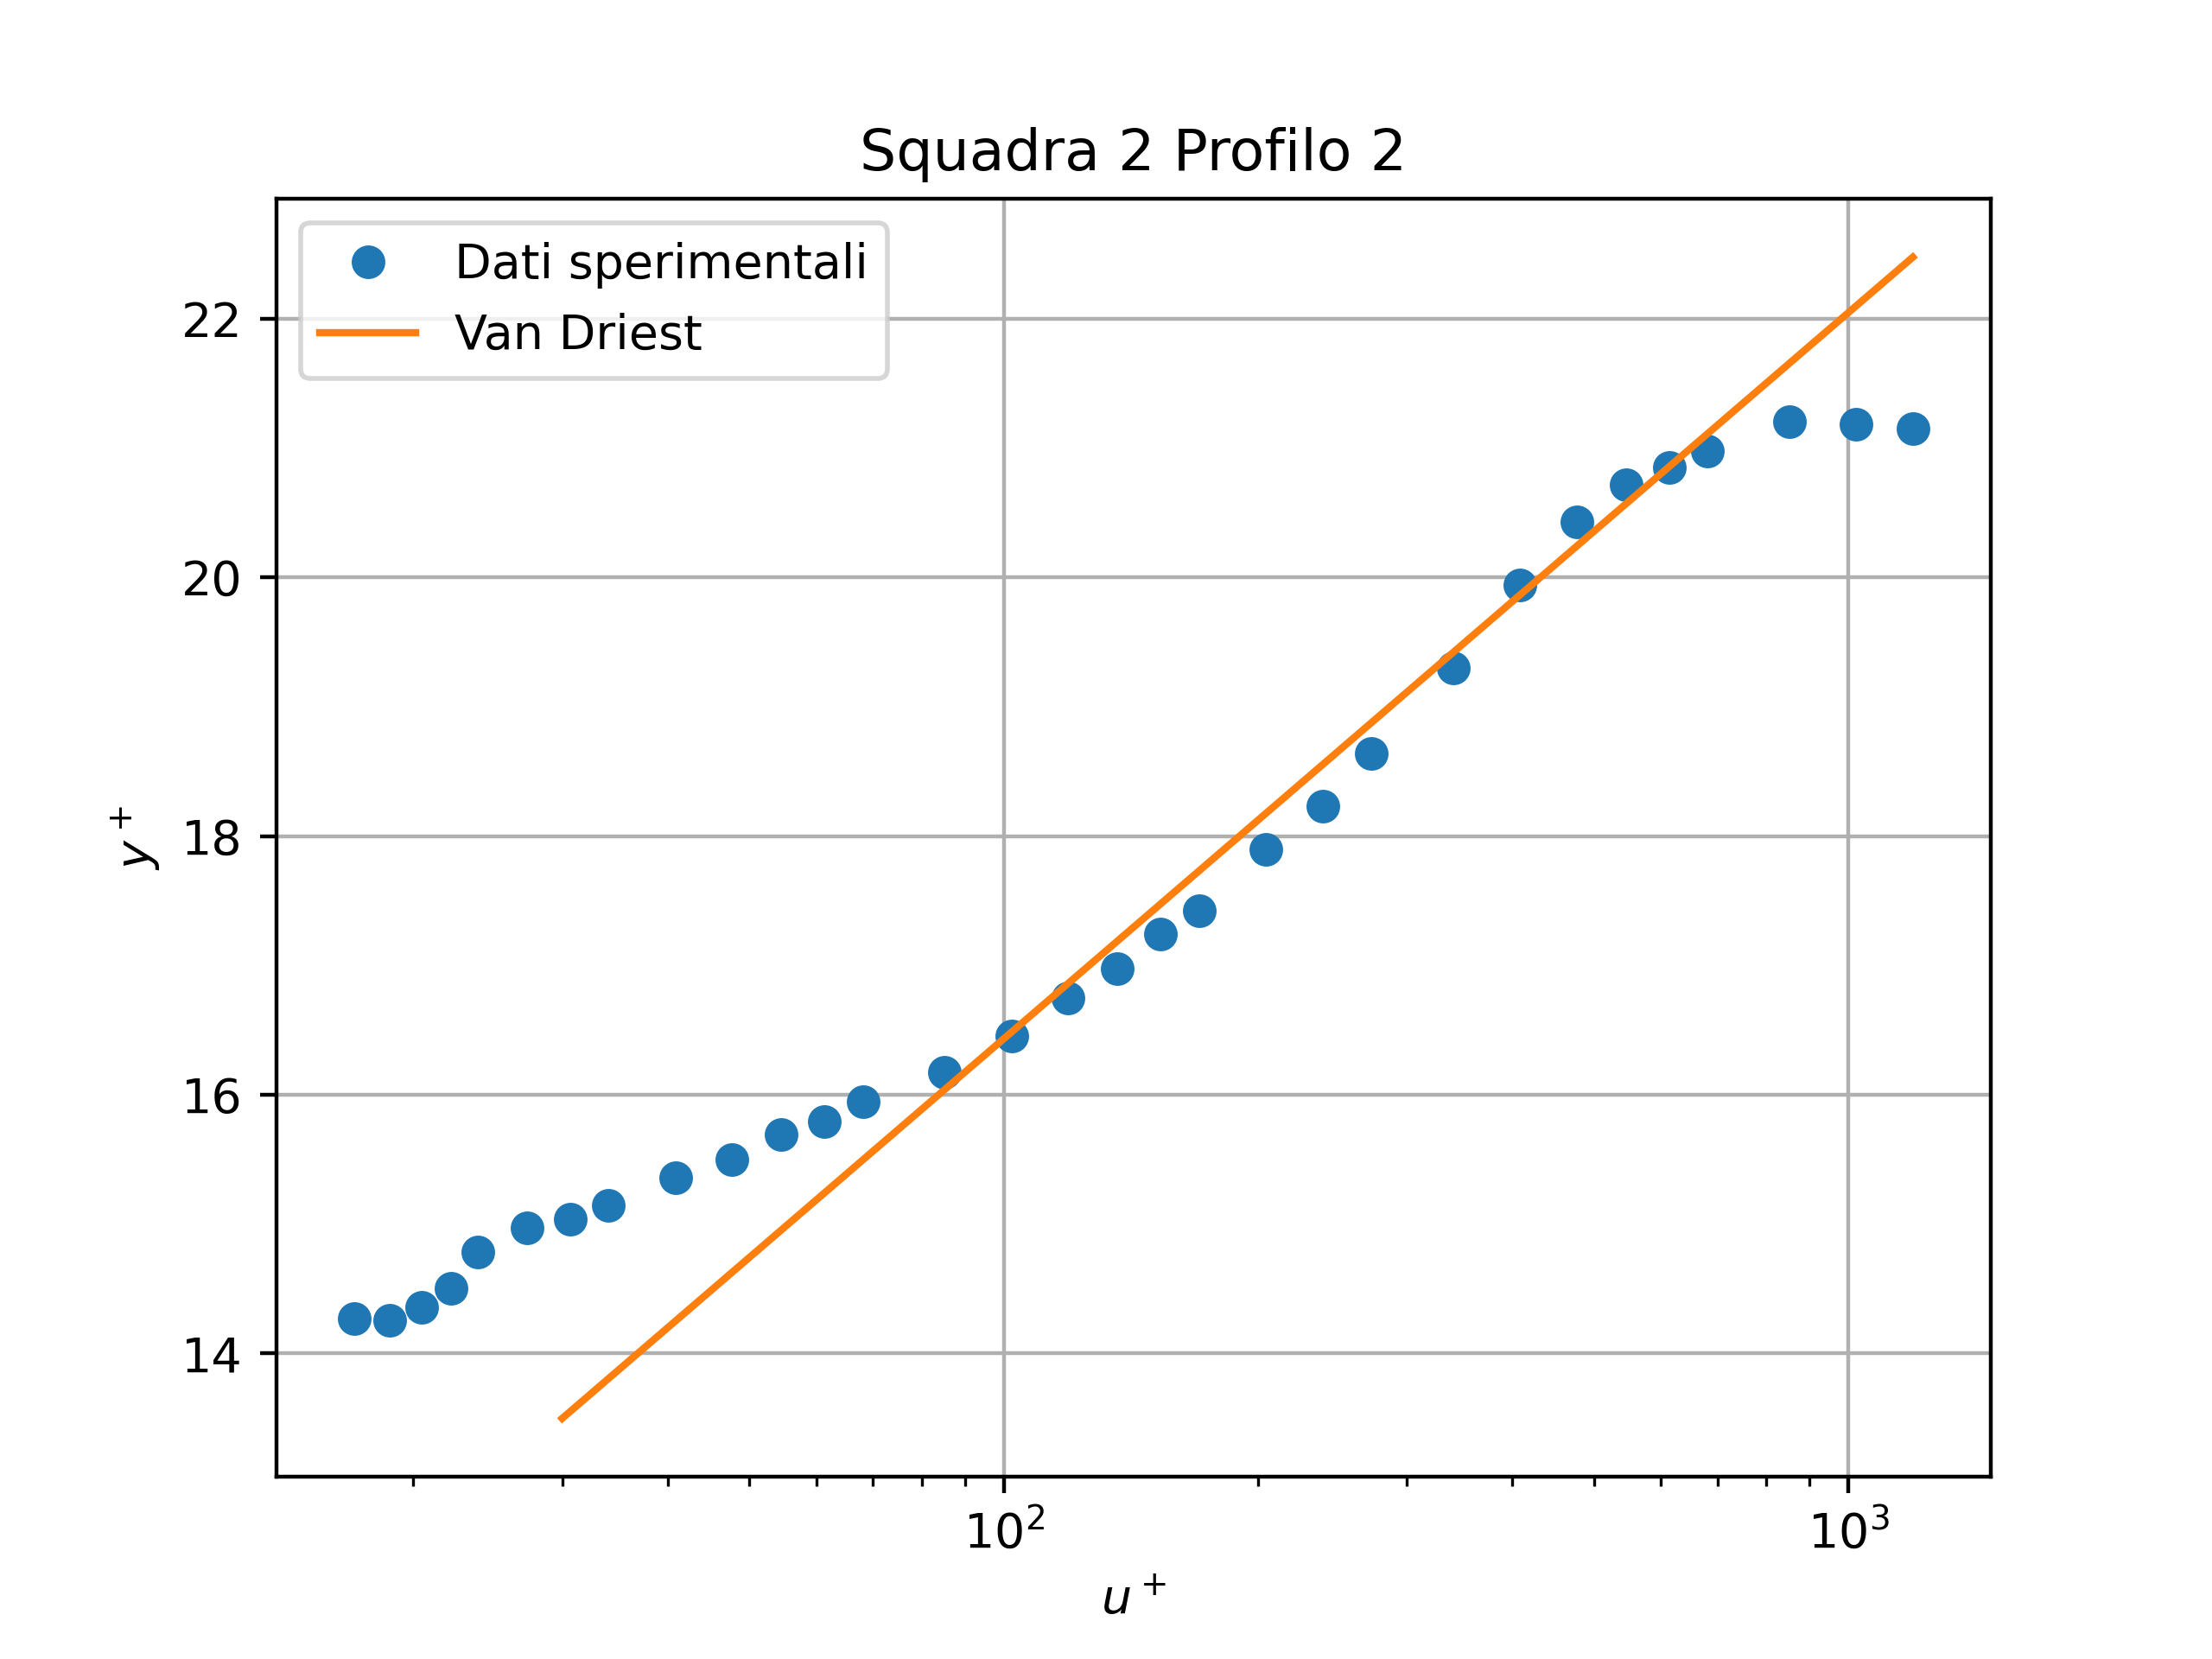
\includegraphics[width=.85\textwidth]{images/9/sq2p2+.png}
    \caption{Diagramma $u^+=f(y^+)$ per la seconda squadra}
\end{figure}

\begin{figure}[H]
    \centering
    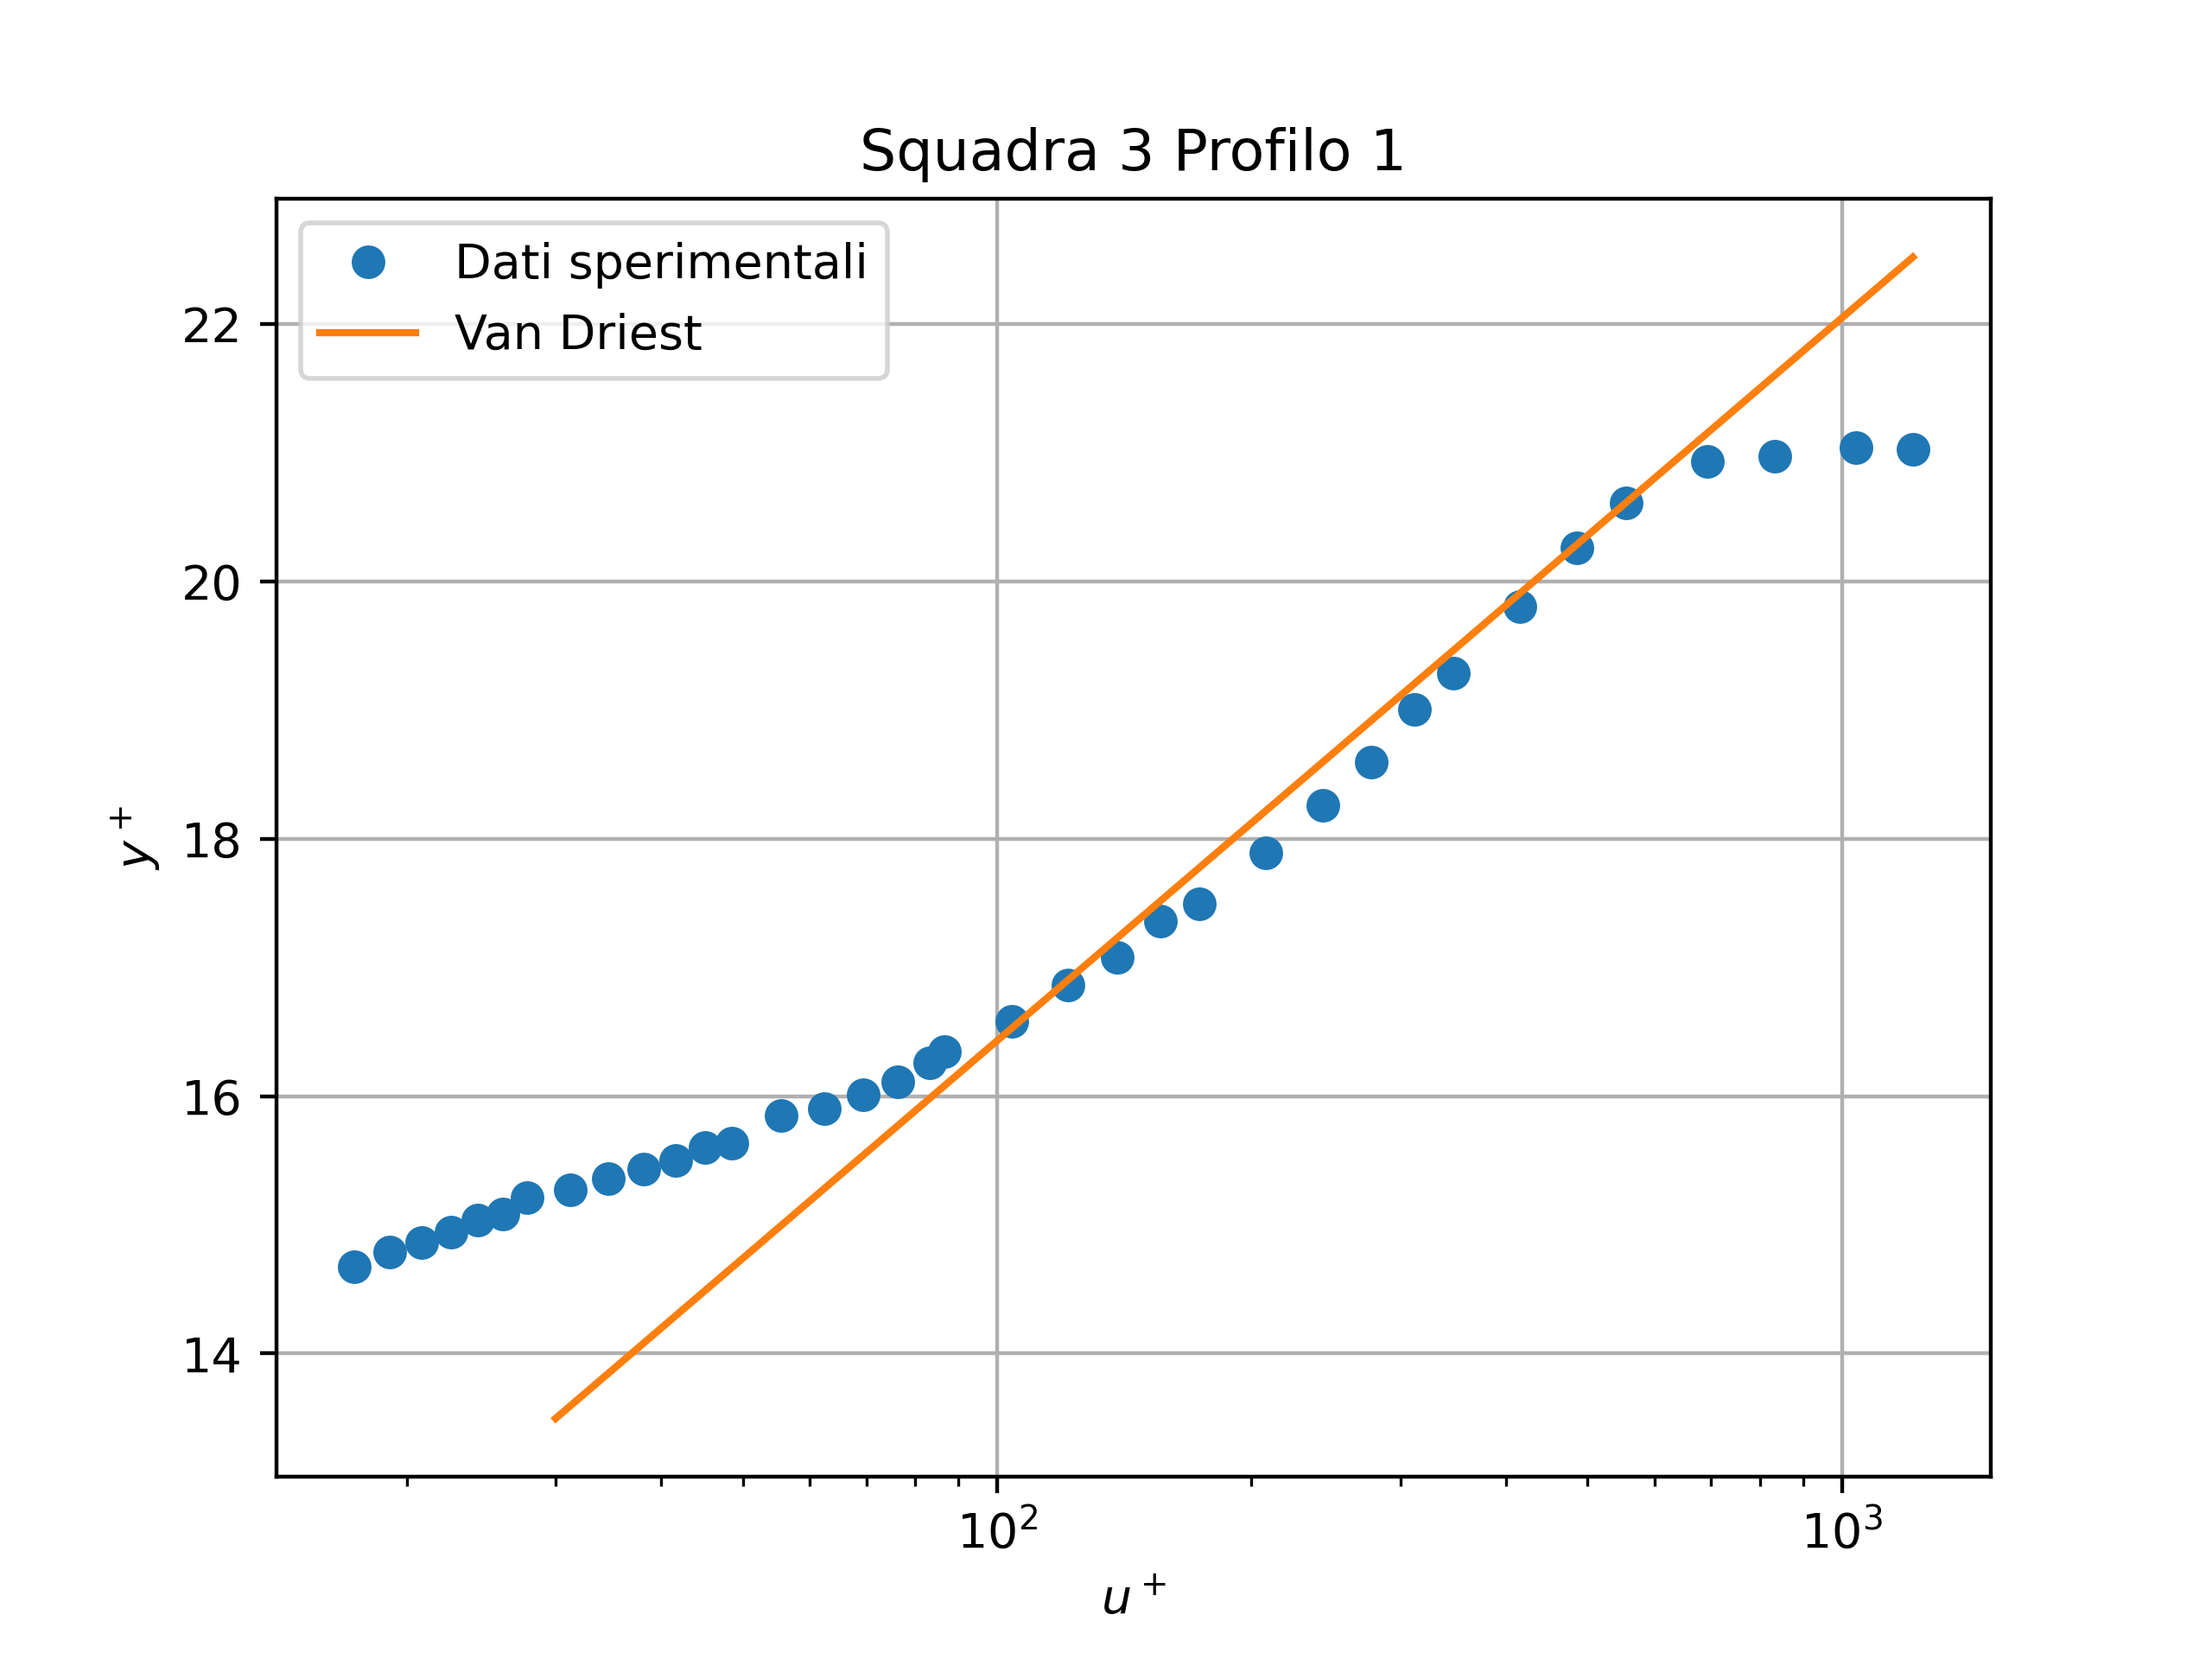
\includegraphics[width=.85\textwidth]{images/9/sq3p1+.png}
    \caption{Diagramma $u^+=f(y^+)$ per la terza squadra}
\end{figure}

\begin{figure}[H]
    \centering
    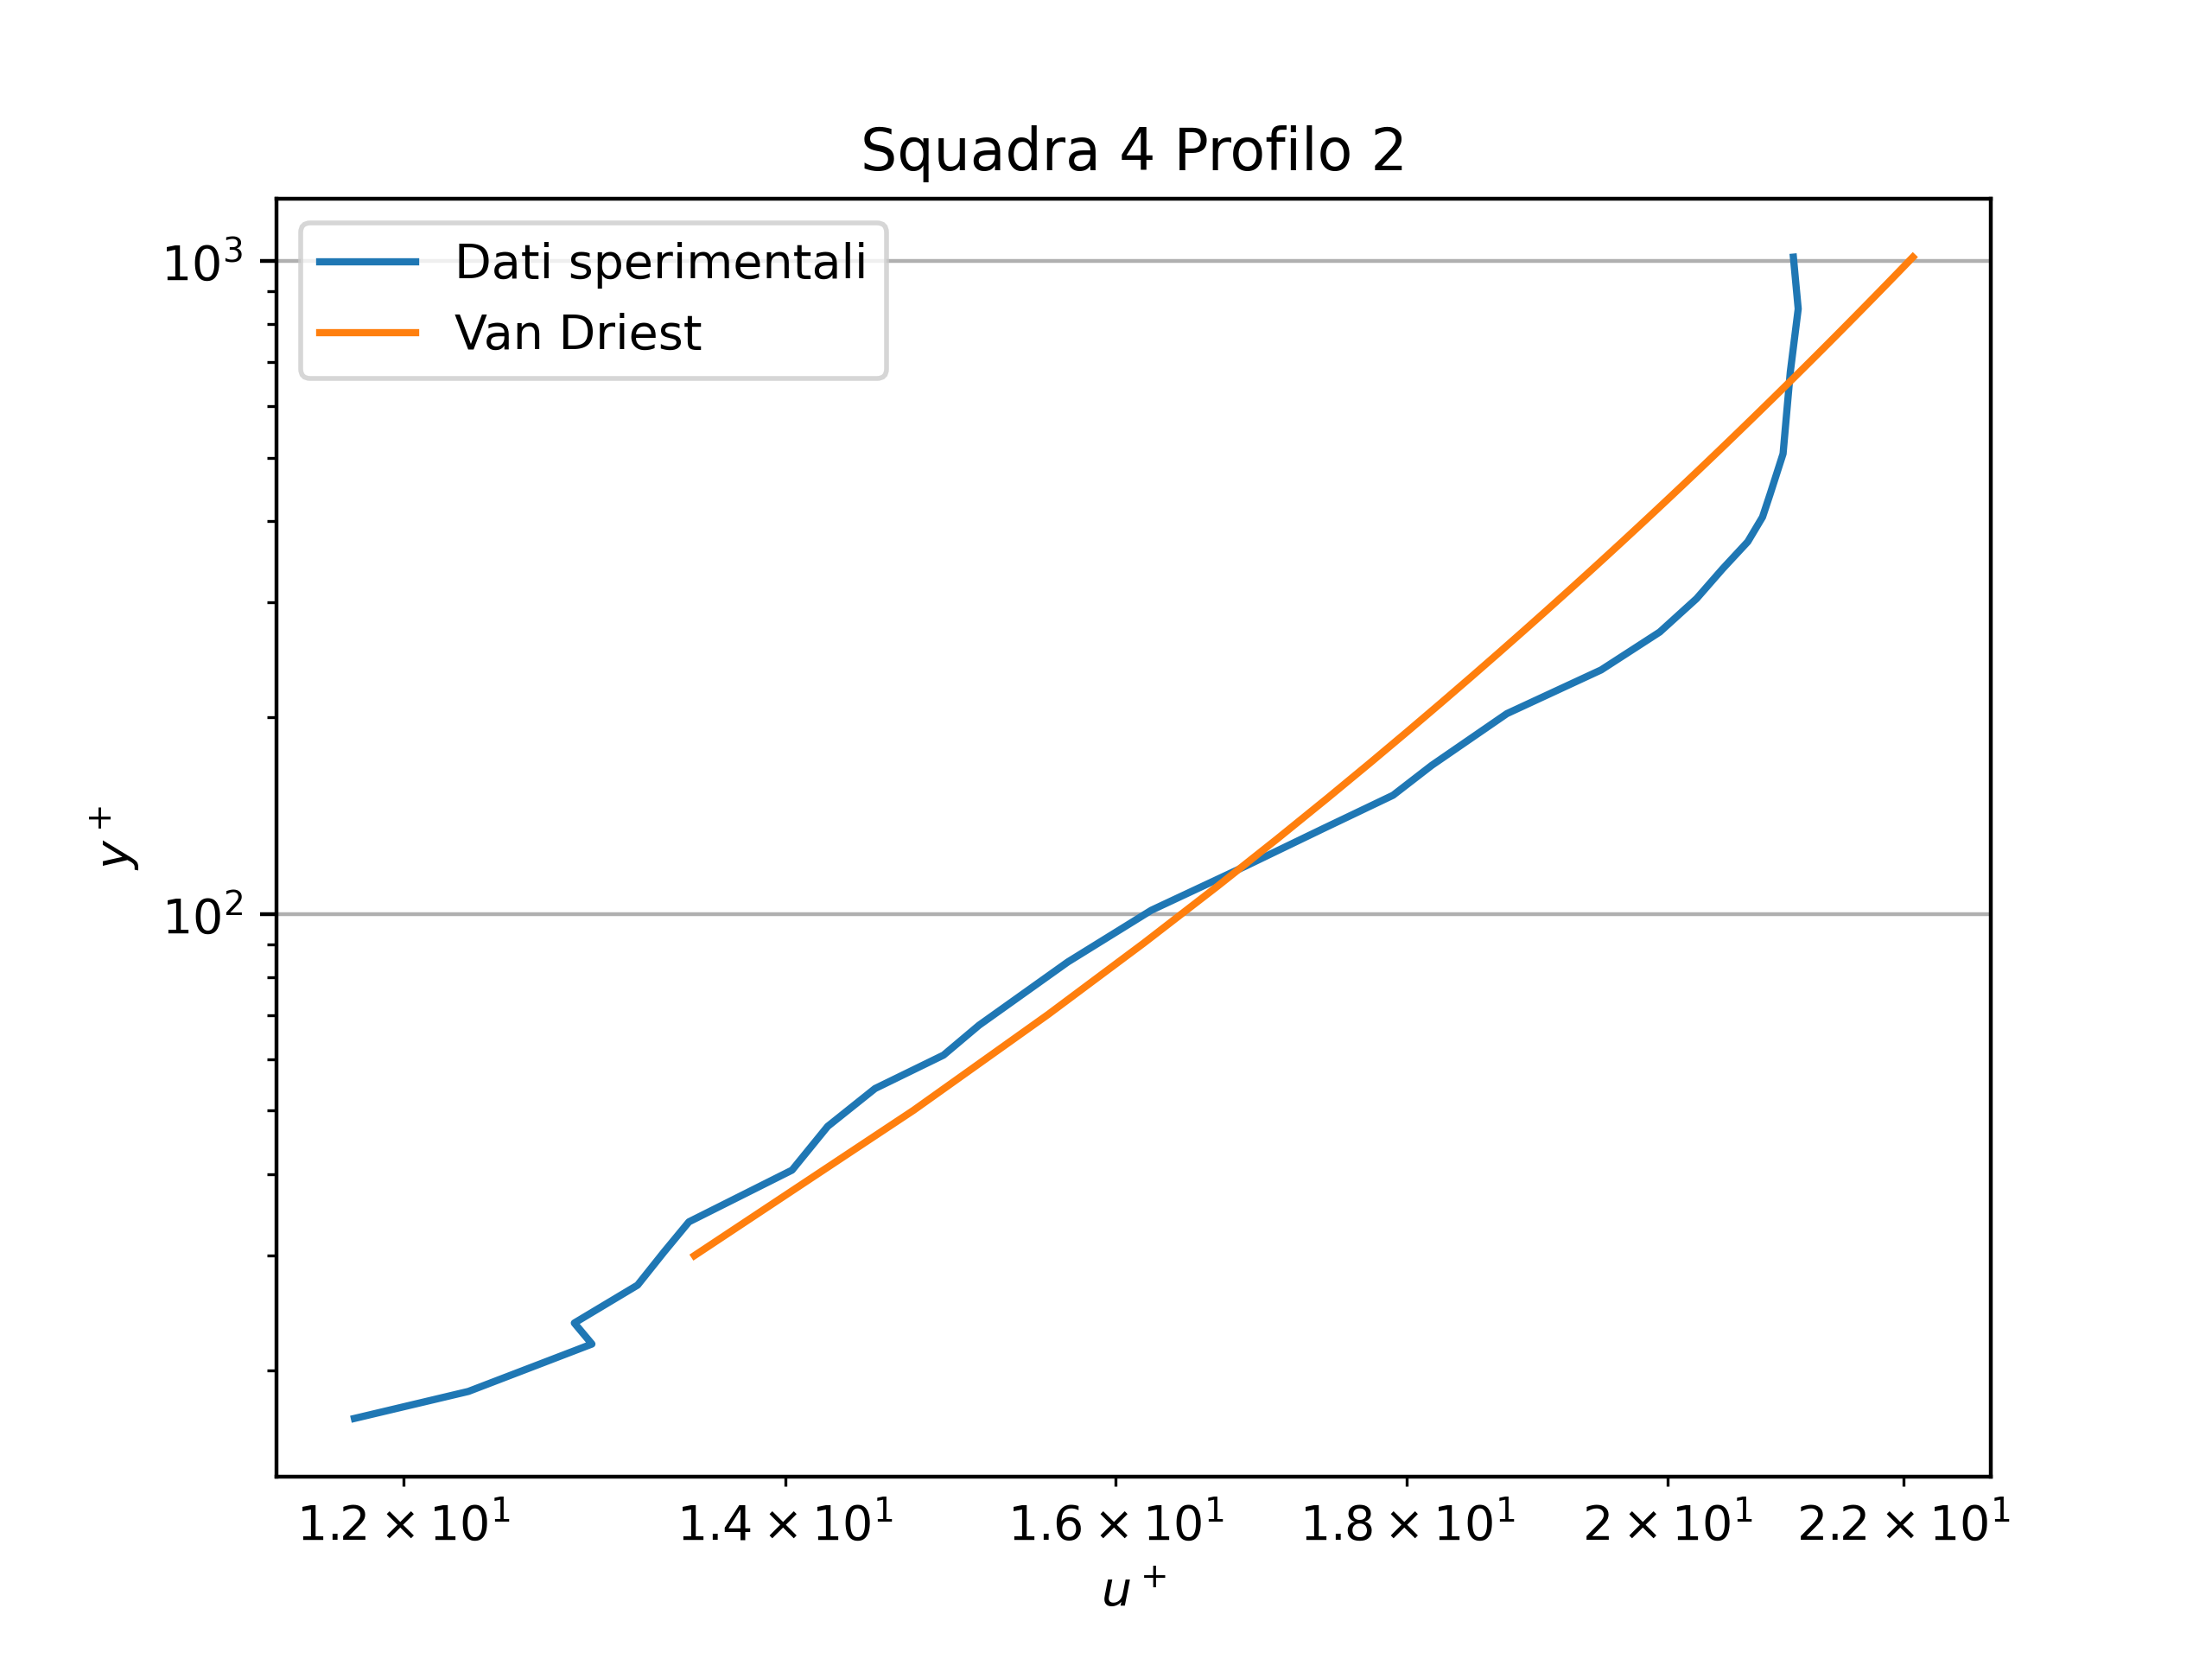
\includegraphics[width=.8\textwidth]{images/9/sq4p2+.png}
    \caption{Diagramma $u^+=f(y^+)$ per la quarta squadra}
\end{figure}

\noindent Si diagrammano inoltre le fluttuazioni adimensionali $u^+_{rms}$ in funzione della coordinata interna $y^+$:
\begin{figure}[H]
    \centering
    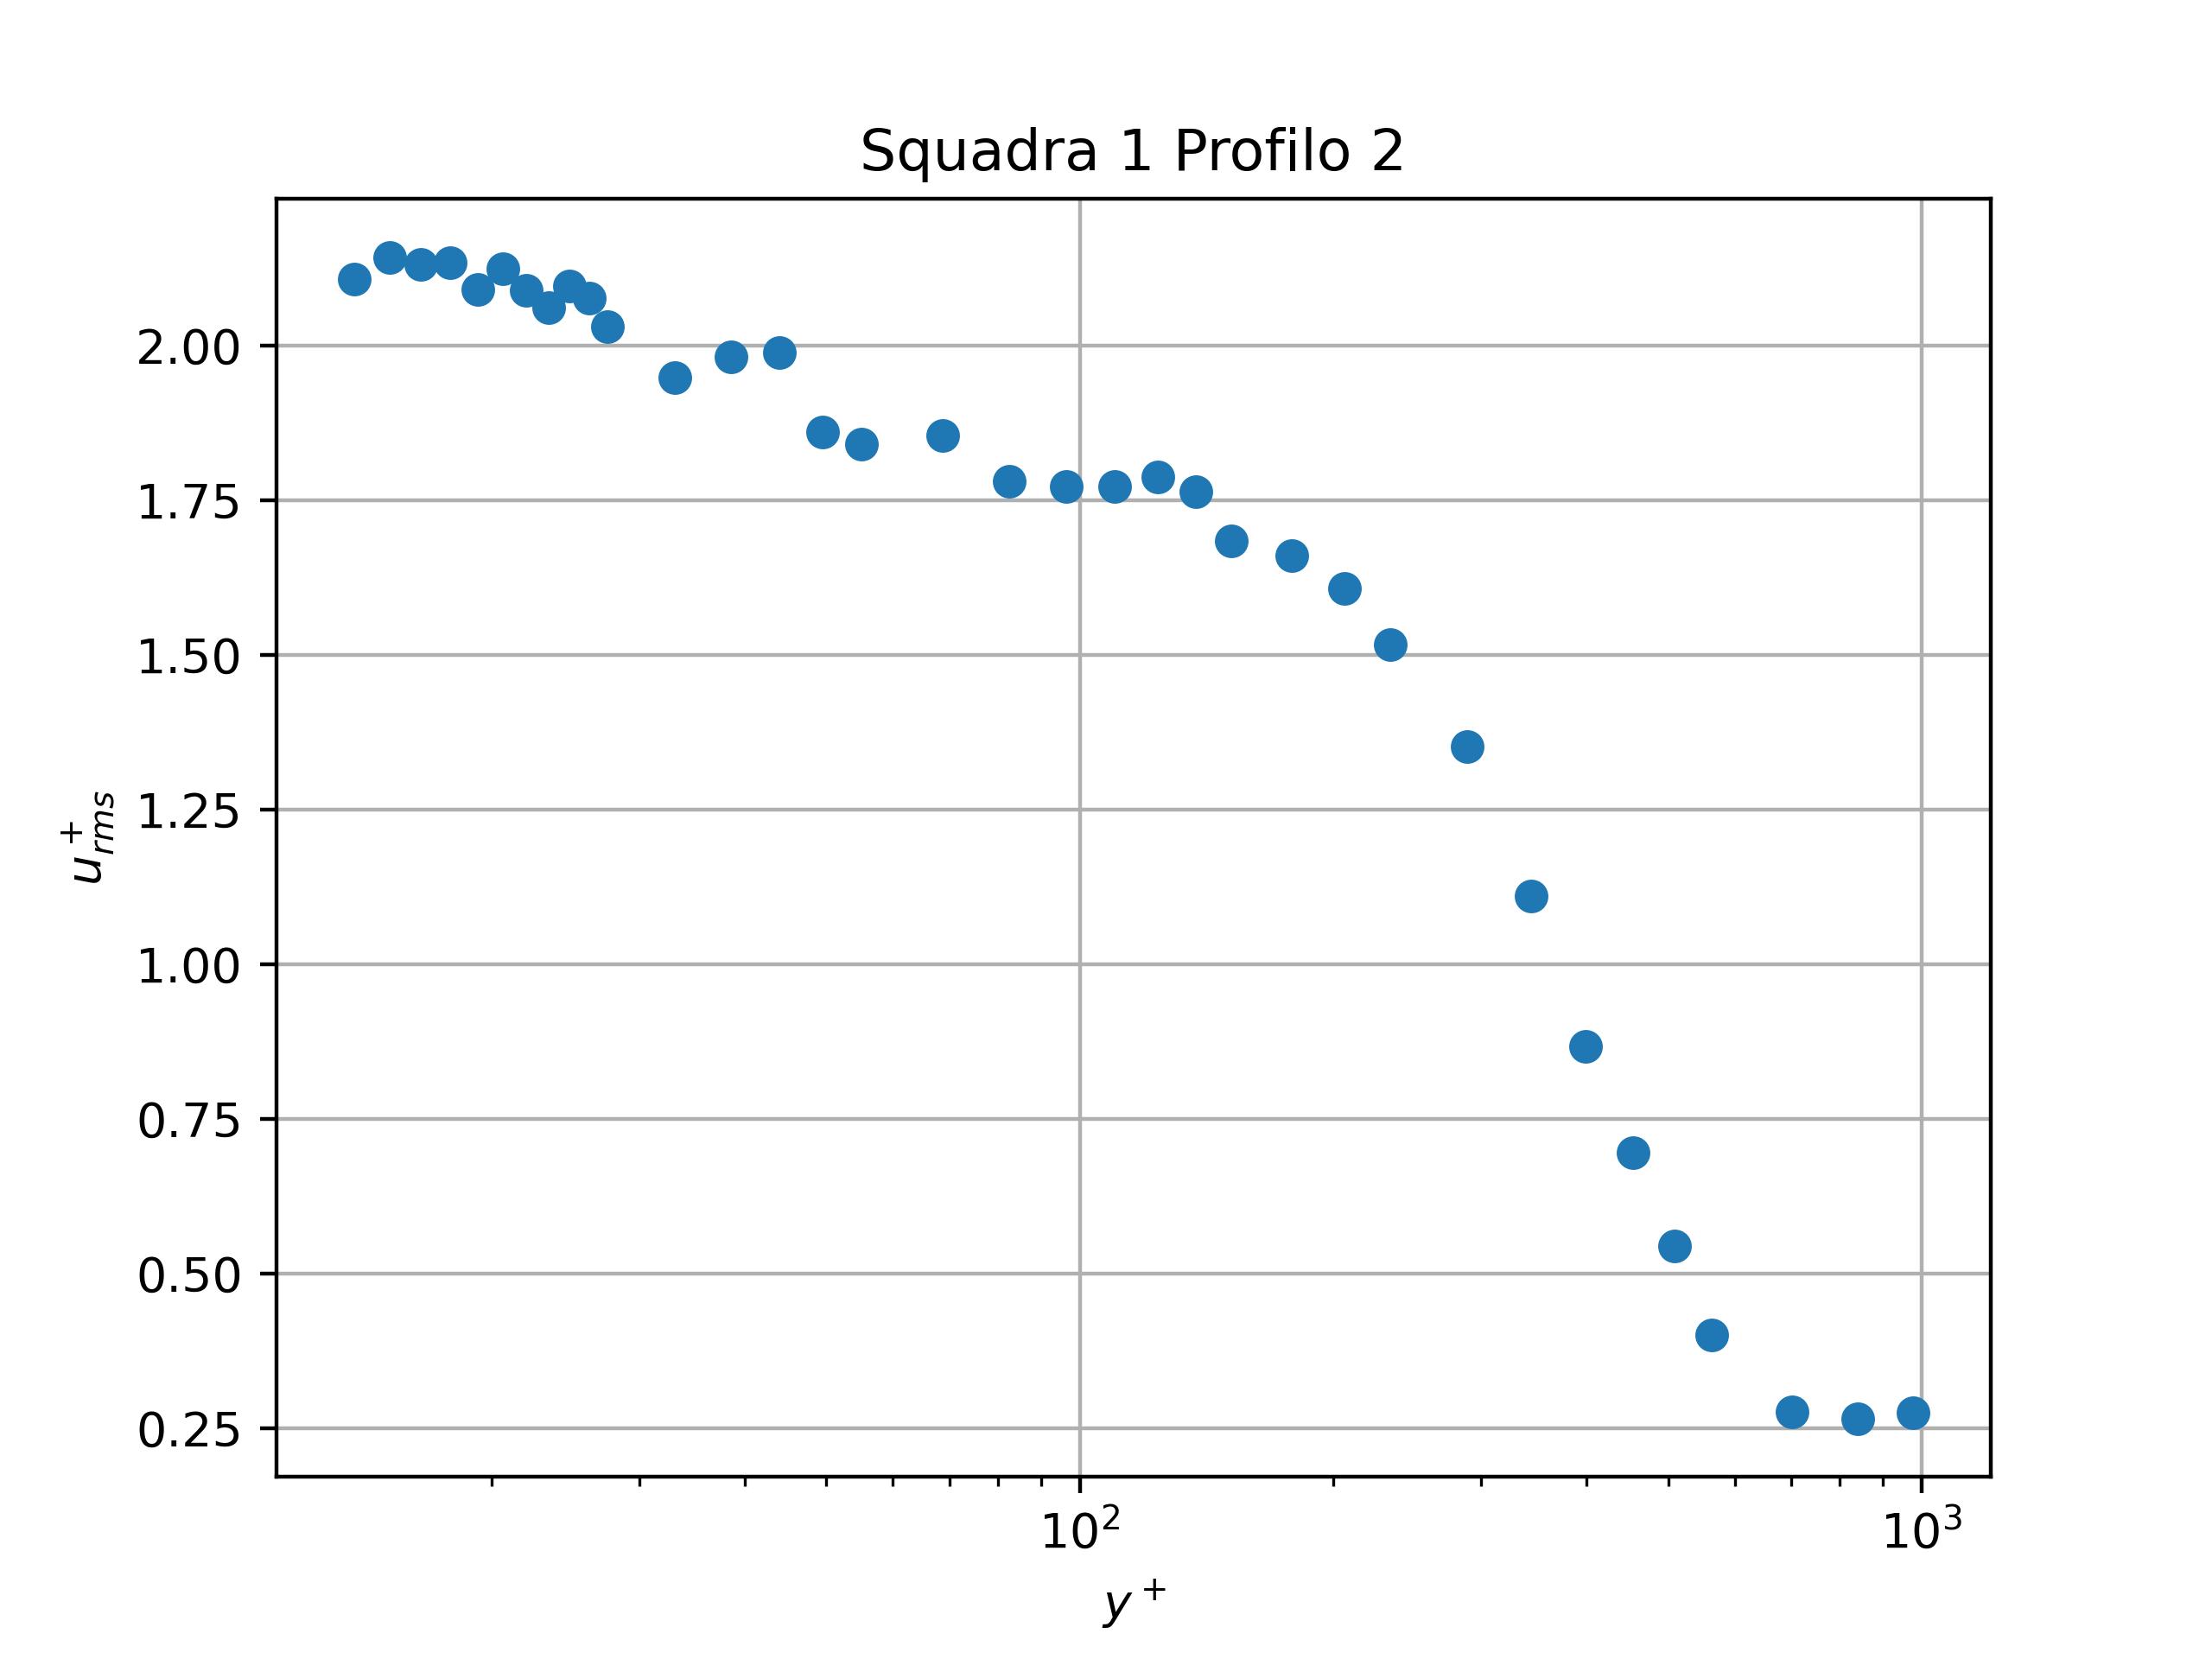
\includegraphics[width=.8\textwidth]{images/9/sq1p2+_rms.png}
    \caption{Fluttuazioni adimensionali $u^+_{rms}=f(y^+)$ per la prima squadra}
\end{figure}

\begin{figure}[H]
    \centering
    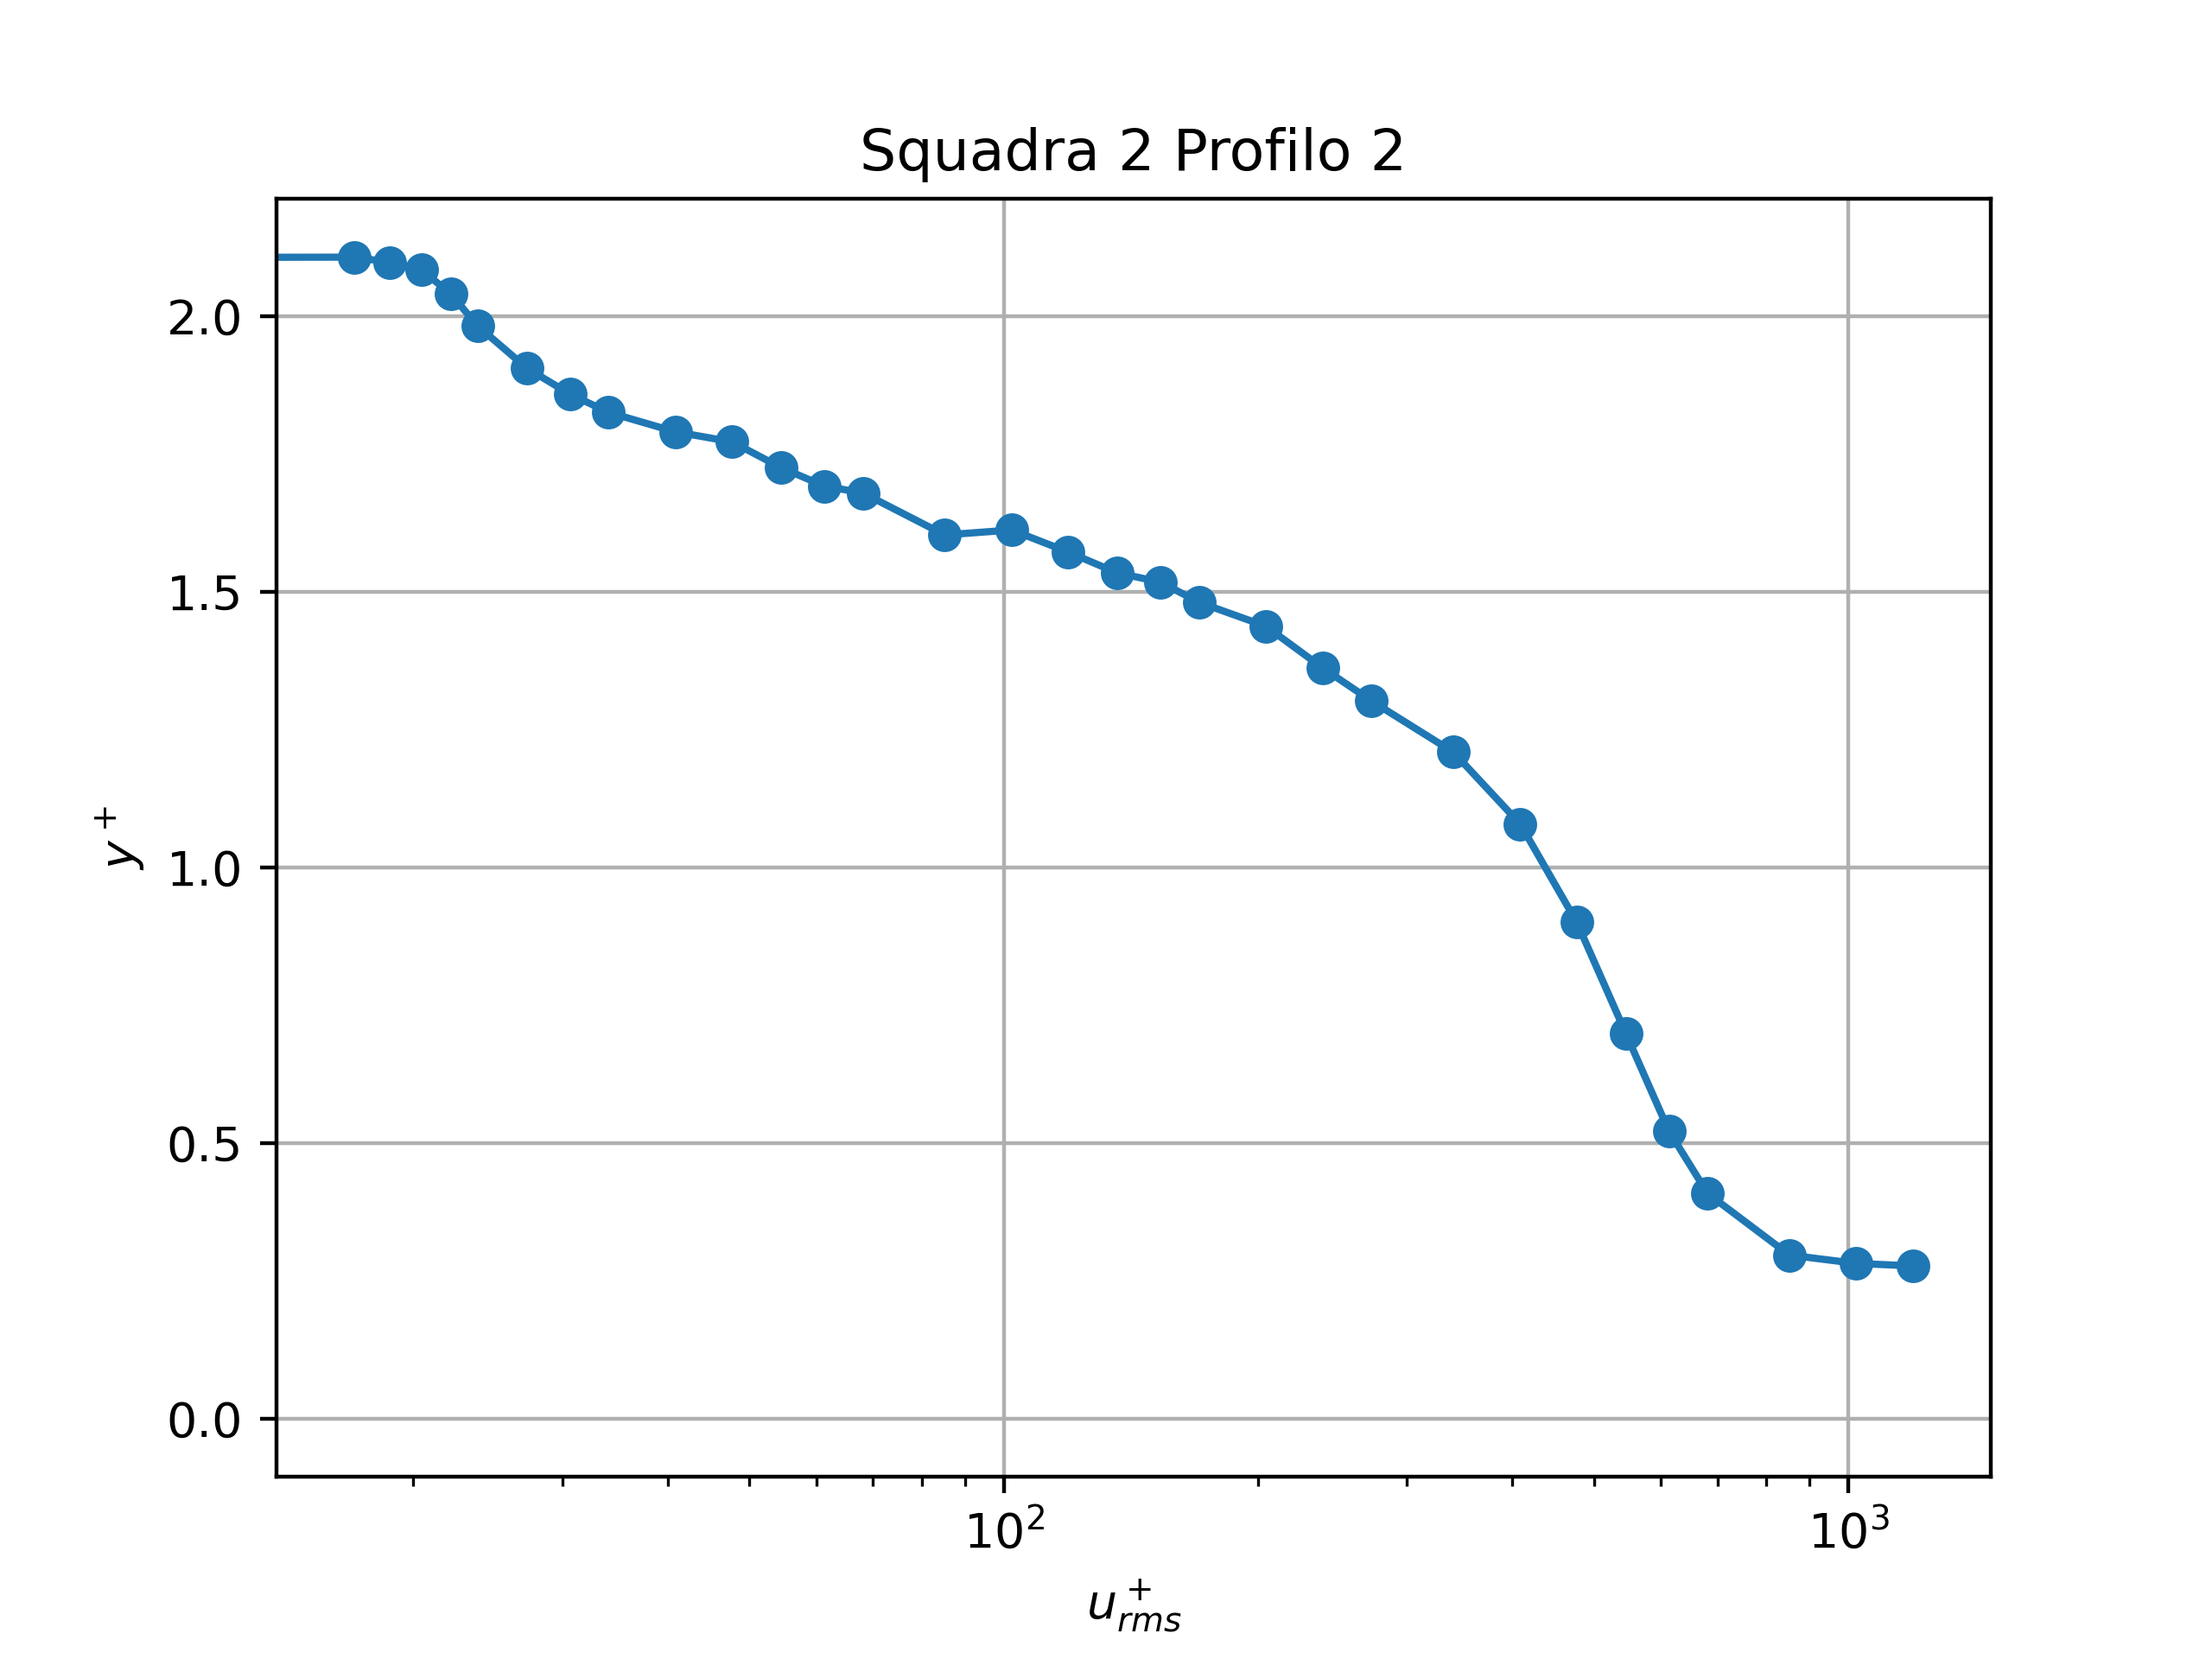
\includegraphics[width=.85\textwidth]{images/9/sq2p2+_rms.png}
    \caption{Fluttuazioni adimensionali $u^+_{rms}=f(y^+)$ per la seconda squadra}
\end{figure}

\begin{figure}[H]
    \centering
    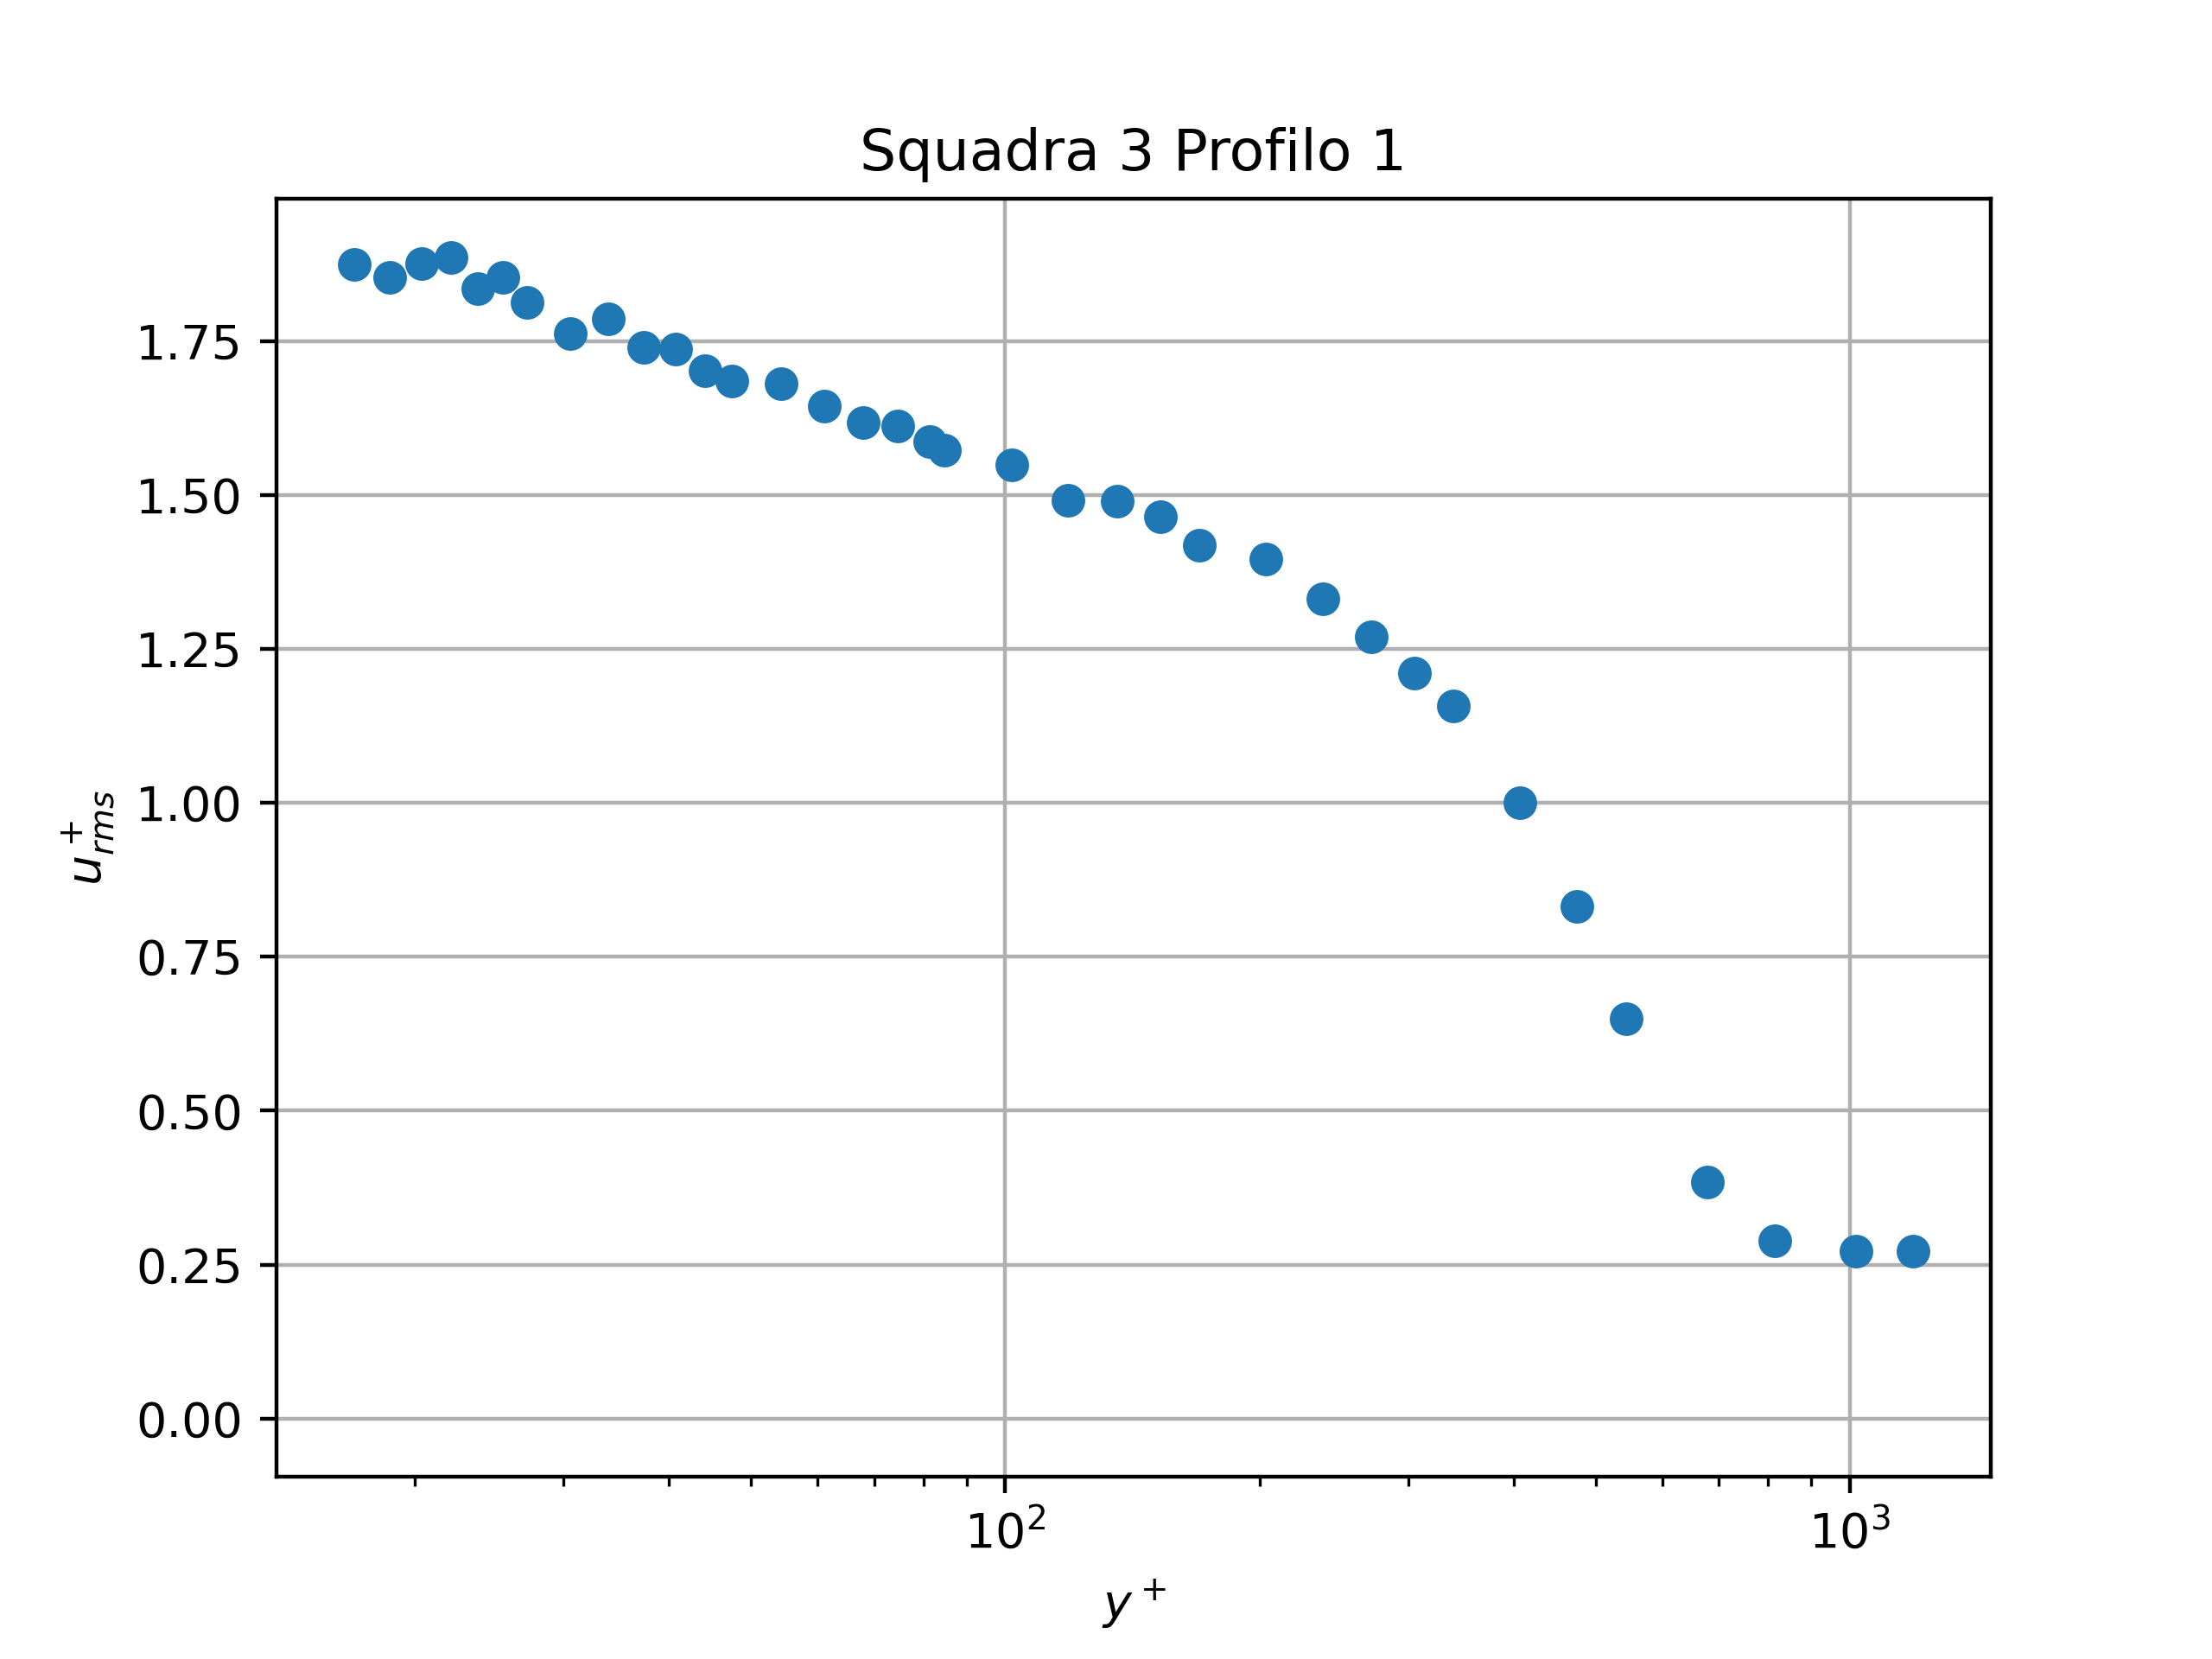
\includegraphics[width=.85\textwidth]{images/9/sq3p1+_rms.png}
    \caption{Fluttuazioni adimensionali $u^+_{rms}=f(y^+)$ per la terza squadra}
\end{figure}

\begin{figure}[H]
    \centering
    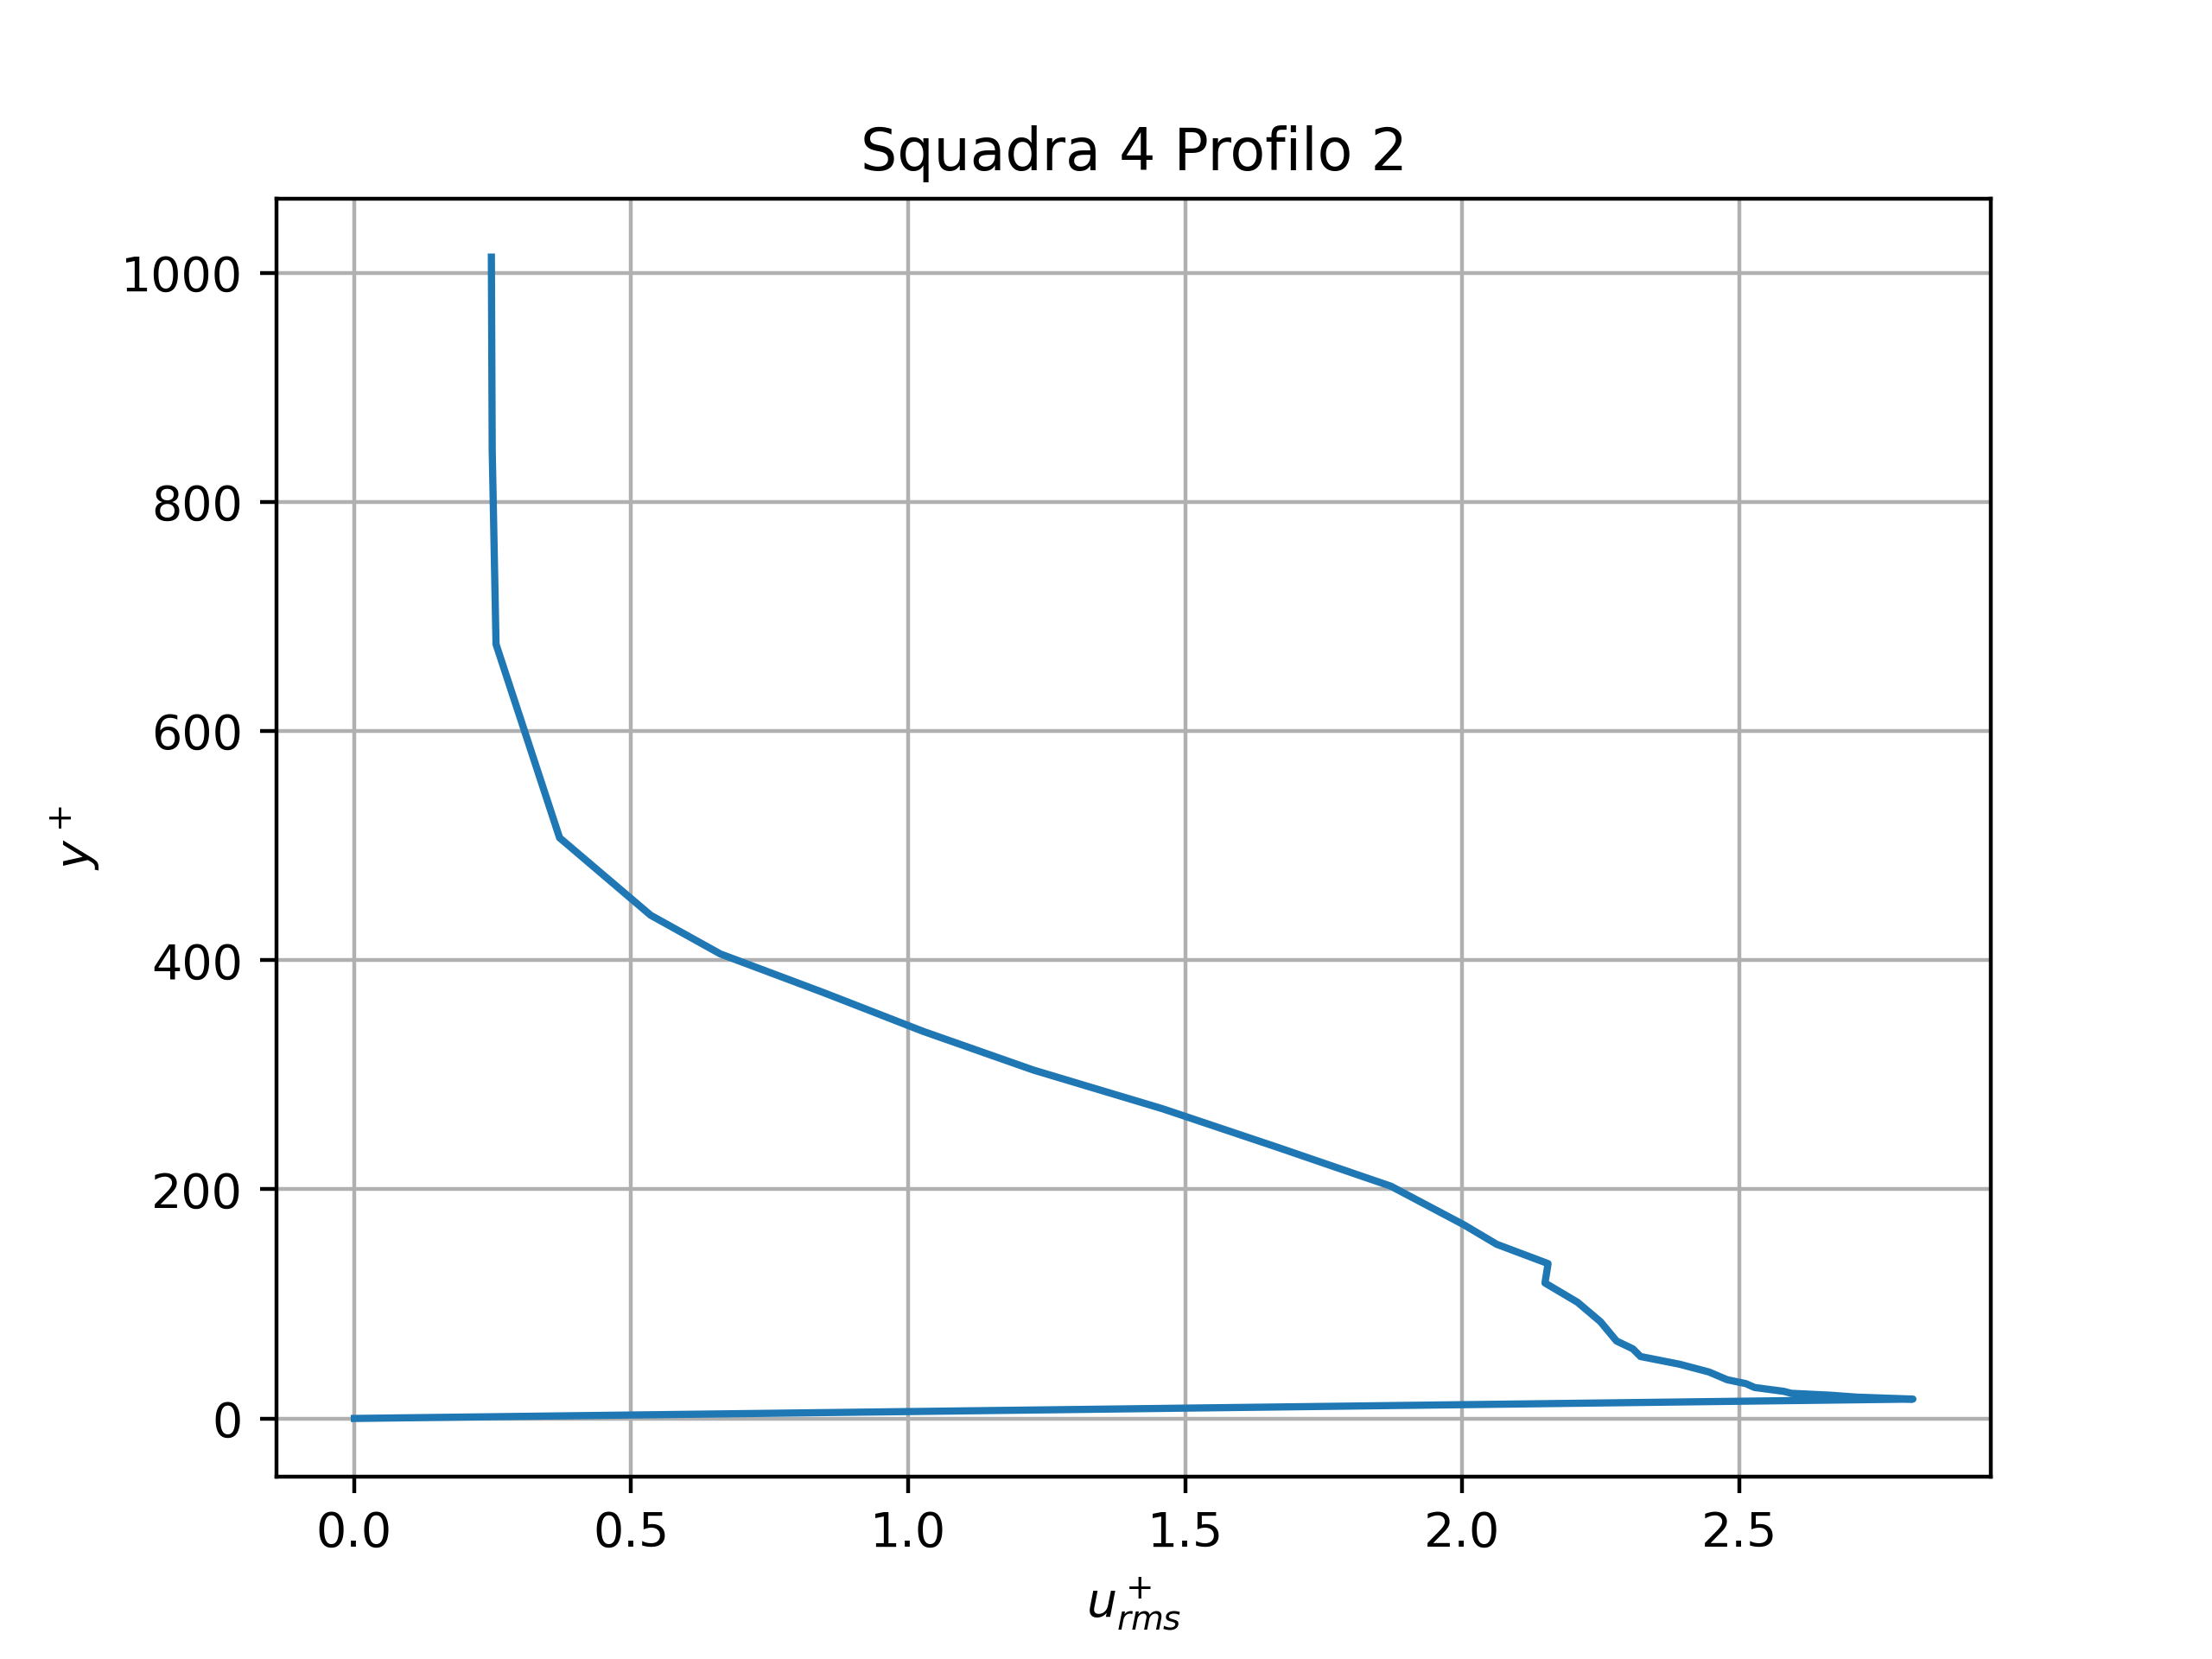
\includegraphics[width=.85\textwidth]{images/9/sq4p2+_rms.png}
    \caption{Fluttuazioni adimensionali $u^+_{rms}=f(y^+)$ per la quarta squadra}
\end{figure}

\noindent Il massimo delle fluttuazioni adimensionali $u^+_{rms}$ si rileva per una coordinata interna $y^+\approx20$, quindi, come previsto dalla teoria, nel buffer layer. Si osserva inoltre dai dati sperimentali che la sonda a filo caldo non ha raggiunto il sottostrato viscoso.

\subsection{Spettro di potenza}
Diagrammando la velocità misurata in funzione del tempo in uno strato limite turbolento, si ottiene:
\begin{figure}[H]
    \centering
    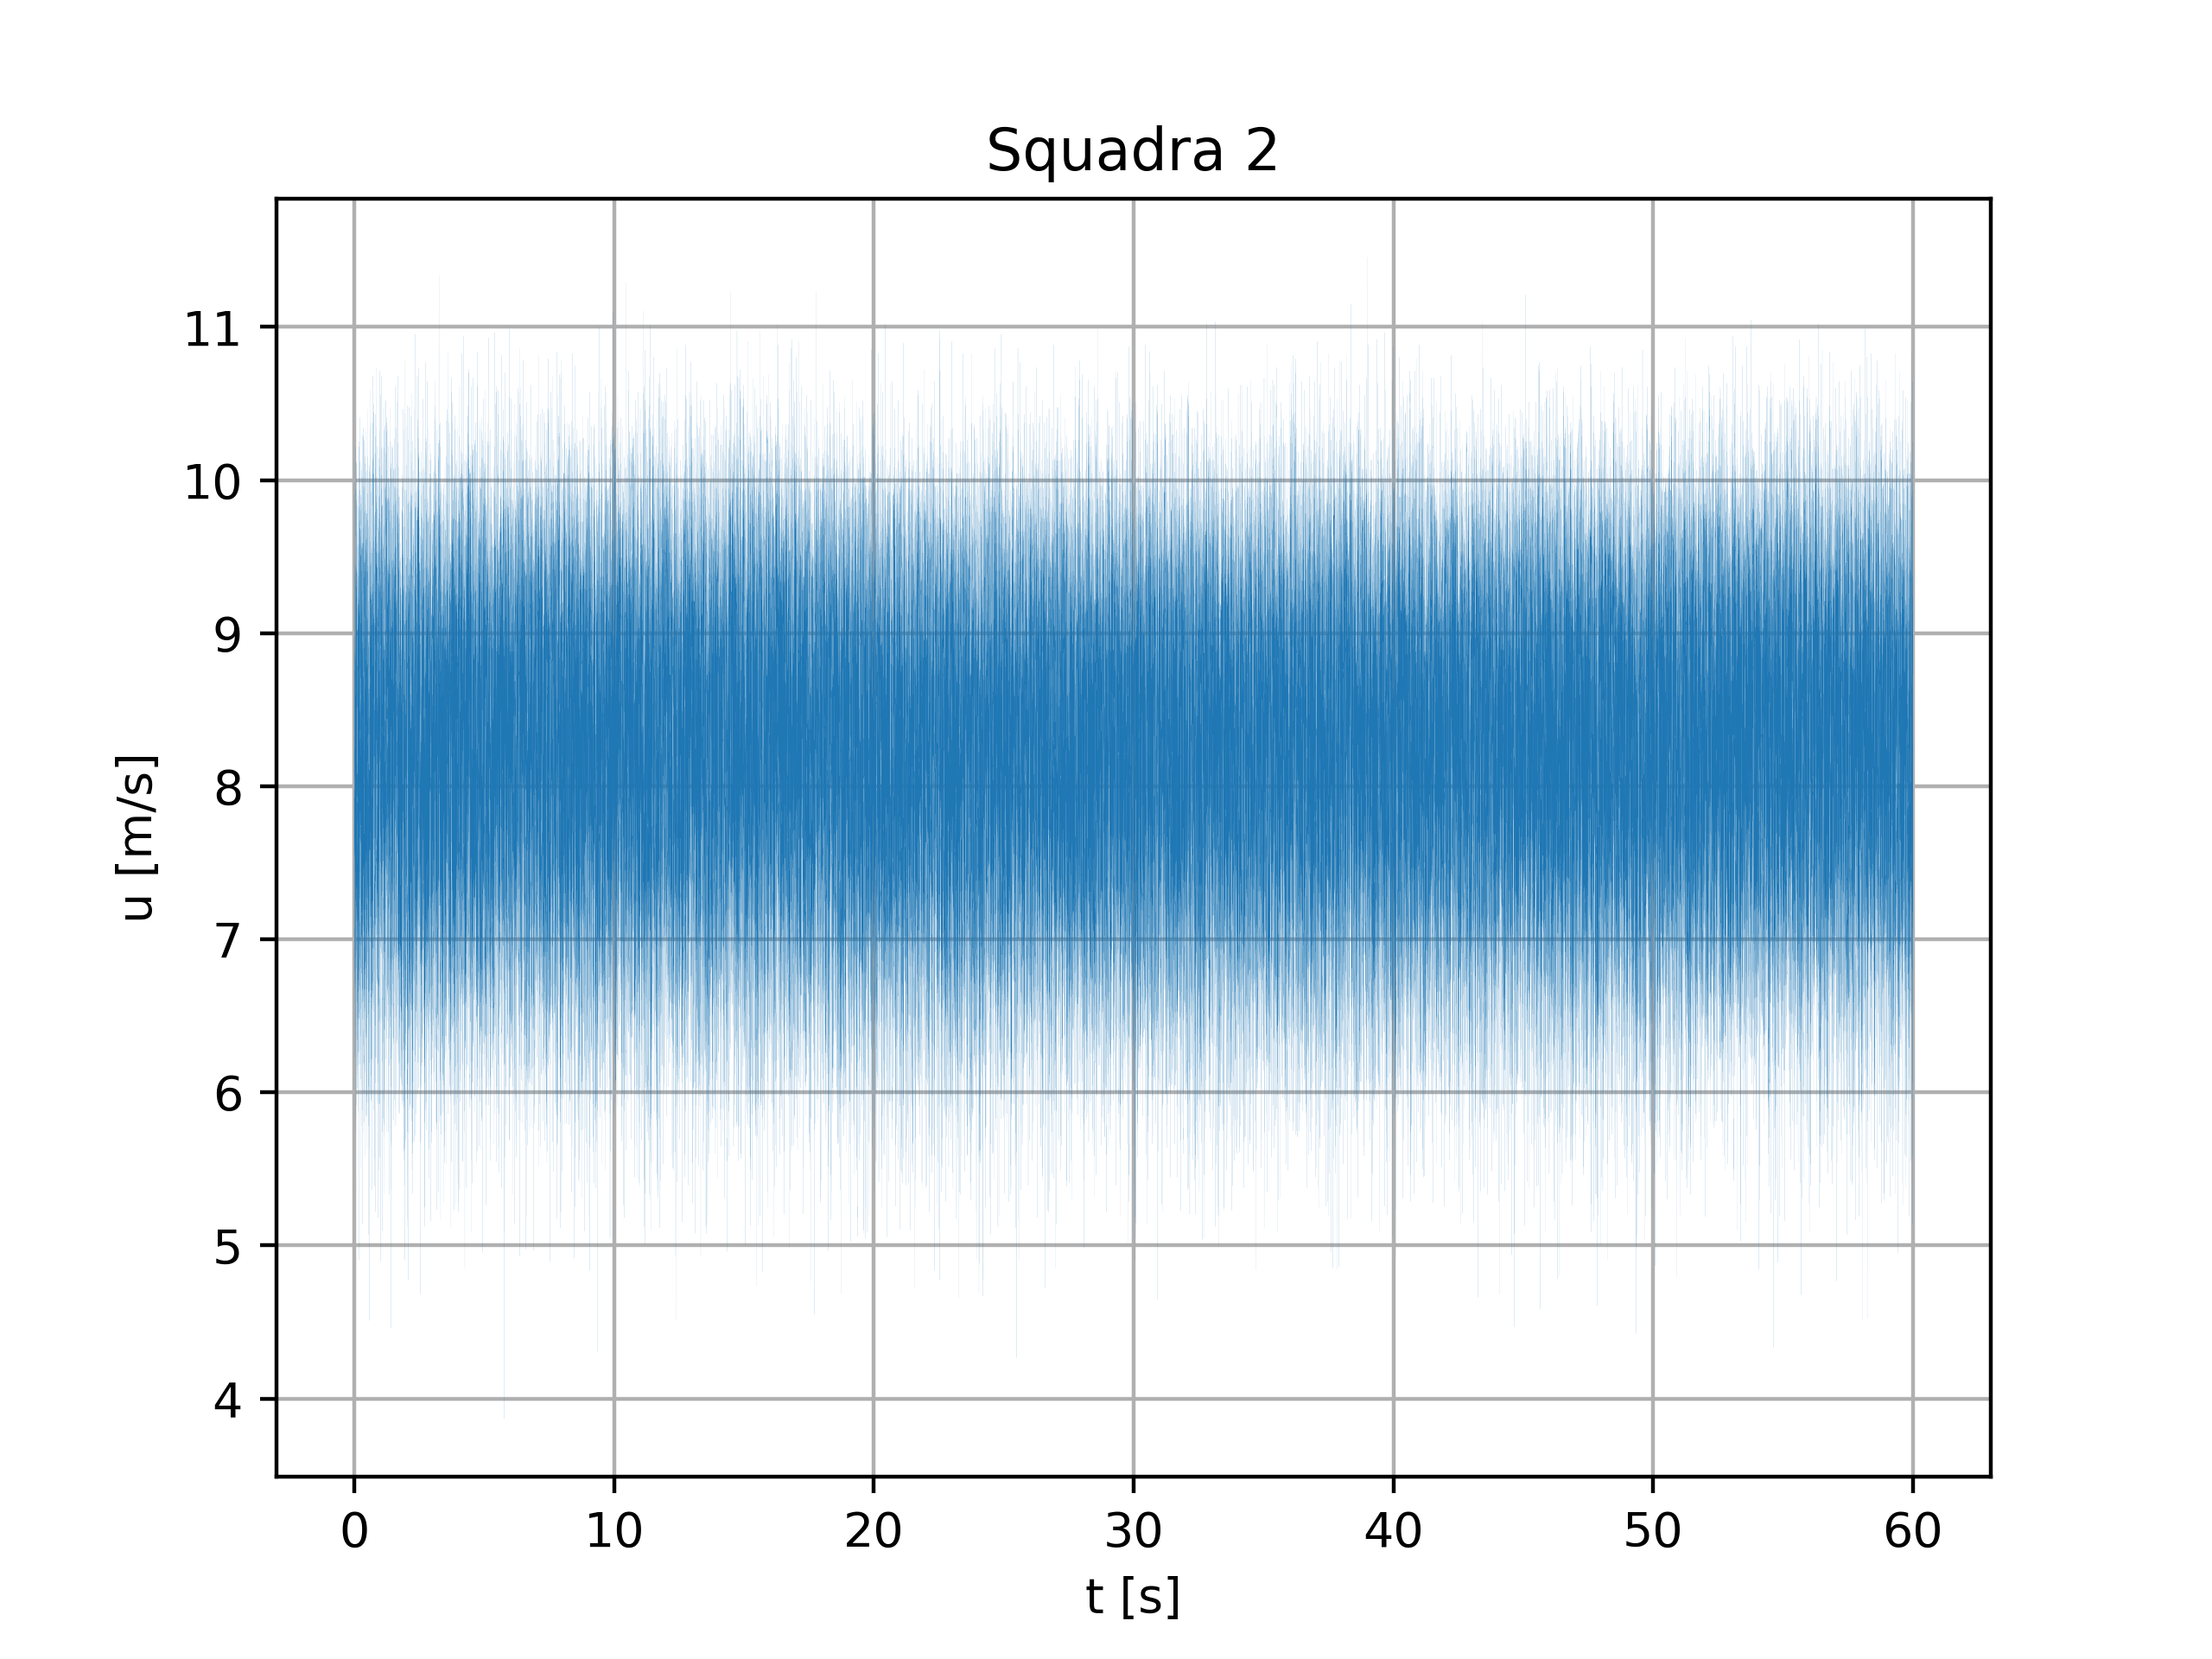
\includegraphics[width=.49\textwidth]{images/9/sq2timeseries.png}
    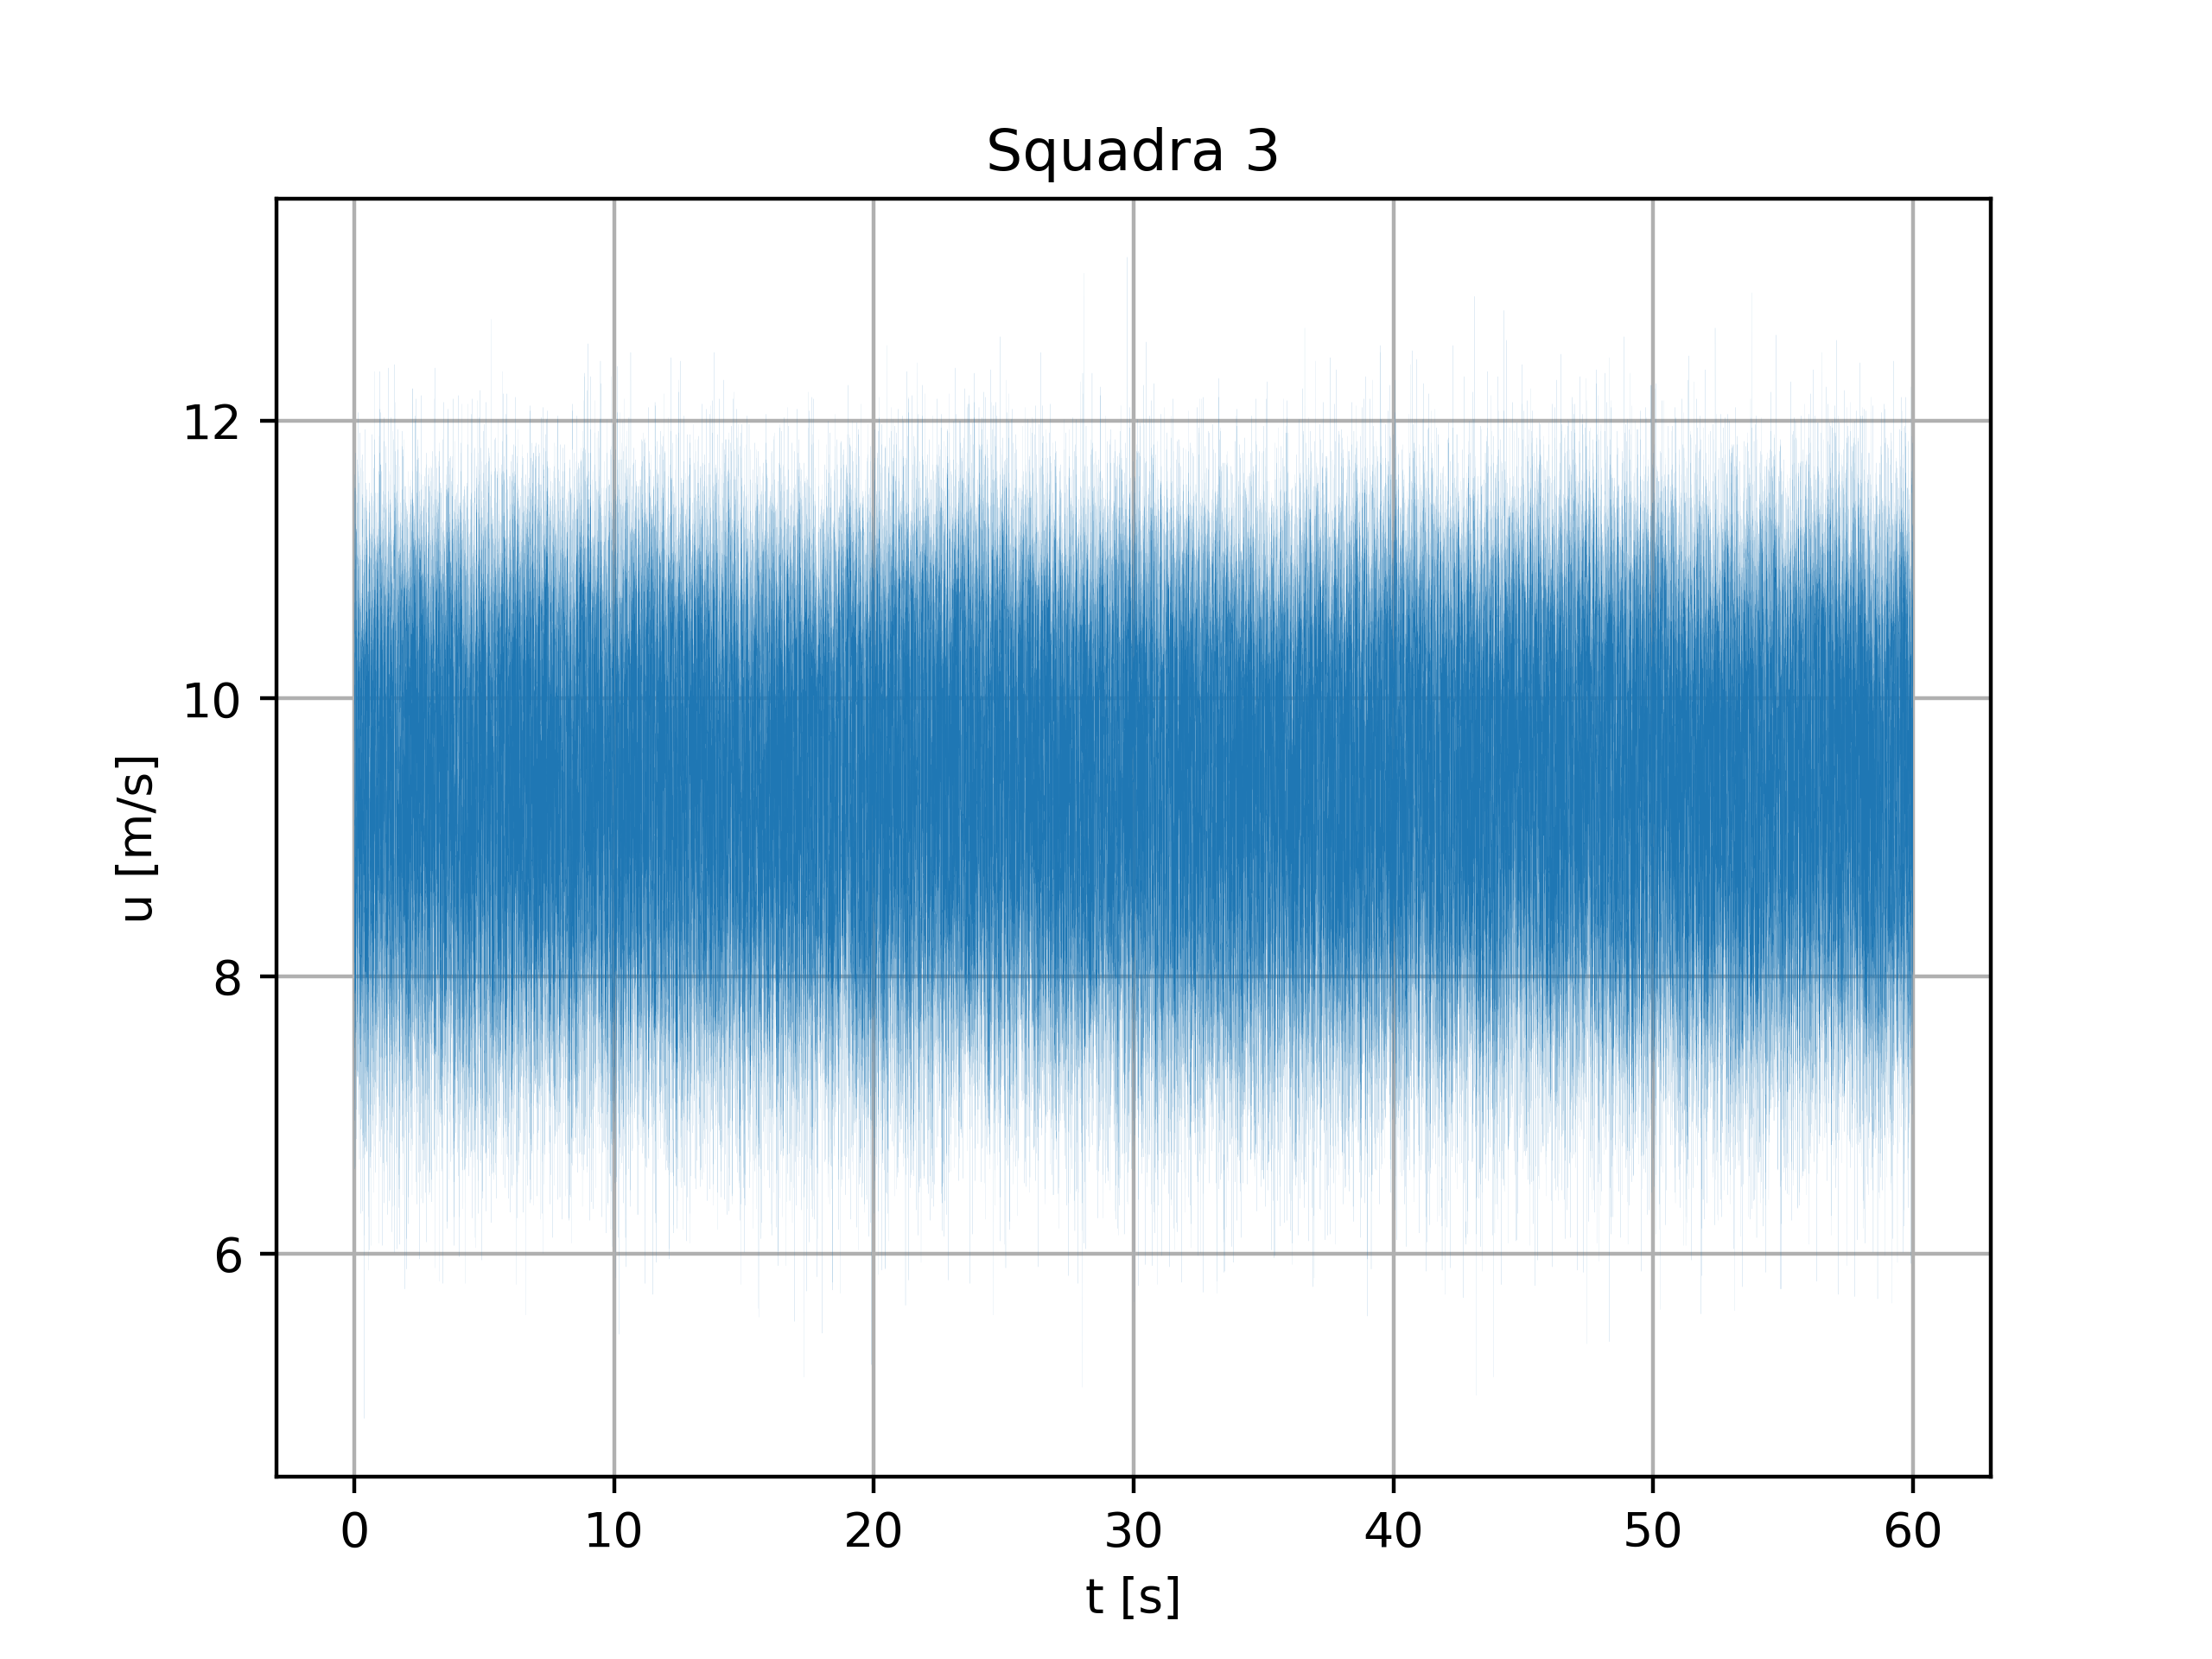
\includegraphics[width=.49\textwidth]{images/9/sq3timeseries.png}
    \caption{Velocità misurata in funzione del tempo $u(t)$ (squadre 2 e 3)}
\end{figure}

\noindent L'analisi nel dominio del tempo permette di esaminare aspetti locali o istantanei in un flusso turbolento, ma non permette di catturare la distribuzione energetica tra diverse scale spaziali e temporali, né di identificare chiaramente le frequenze dominanti e le interazioni complesse all'interno del flusso.\\\\
Un'analisi nel dominio delle frequenze, invece, offre una prospettiva più completa delle caratteristiche spettrali e dinamiche del flusso.\\\\
Per eseguire un'analisi in frequenza, ogni squadra ha effettuato una misura ad un'elevata frequenza di campionamento (fs = 30 kHz, per la quarta squadra fs = 20 kHz) per un periodo $T$ di un minuto (55 secondi per la squadra 4).\\\\
Dai segnali di tensione in uscita $E_i$ rilevati dalla sonda a filo caldo si ricavano i valori di velocità $U_i$ utilizzando la legge di King:
\begin{equation*}
    U_i = \left( \frac{E_i^2-A}B \right)^{1/n}
\end{equation*}
Si prosegue utilizzando il metodo di Welch, una tecnica per stimare la densità spettrale di potenza (PSD) di un segnale. Il metodo di Welch suddivide il segnale originale in segmenti sovrapposti, applica una finestra a ciascun segmento, calcola la trasformata di Fourier e stima la PSD per ciascuna finestra ed infine fa una media per ottenere la stima finale della PSD con una varianza ridotta.\\\\
Il segnale in questione, relativo agli $N$ valori della velocità misurata $U[i]$, è quindi suddiviso in $K$ segmenti sovrapposti di lunghezza $L$, con una sovrapposizione di $D$ campioni. Il numero di segmenti è dato da:
\begin{equation*}
    K = \frac{N-D}{L-D}
\end{equation*}
Per ogni indice $k$, dove $k=0,1,...,K-1$, si considera il segmento:
\begin{equation*}
    U_k[i] = \left\{U[i+k(L-D)]\right\} \text{ per } i=0,1,...,L-1
\end{equation*}
Su ogni segmento si applica una finestra $w[i]$ di lunghezza $L$, ottenendo quindi il segnale finestrato:
\begin{equation*}
    U_k^w[i] = U_k[i]w[i]
\end{equation*}
Applicare una finestra significa moltiplicare ogni segmento del segnale con una funzione finestra, questo processo è importante per ridurre effetti indesiderati dovuti alla discontinuità ai bordi dei segmenti. In particolare, nel caso in esame è applicata una finestra di Hanning (Hann), caratterizzata da una forma coseno che riduce dolcemente i valori verso zero ai bordi:
\begin{equation*}
    w[n] = 0.5\left(1-\cos\left( \frac{2\pi n}{N-1} \right)\right)
\end{equation*}
Per ogni segmento finestrato $U_k^w[i]$, si calcola la trasformata di Fourier discreta (DFT):
\begin{equation*}
    \hat U_k^w[f] = \sum_{i=0}^{L-1} U_k^w[i]e^{-j2\pi fi/L}
\end{equation*}
Dove $f=0,1,...,L-1$ sono gli indici di frequenza.\\\\
Successivamente, si stima la PSD per ciascun segmento $k$:
\begin{equation*}
    P_k[f] = \frac 1L \left| \hat U_k^w[f] \right|^2
\end{equation*}
La stima finale della PSD è ottenuta mediando le stime di PSD di ciascun segmento:
\begin{equation*}
    P[f] = \frac 1K \sum_{k=0}^{K-1} P_k[f]
\end{equation*}
Considerando un numero di punti per segmento pari a $L=N/100$ ed un numero di punti in sovrapposizione pari a $D=L/2$, si ottengono i seguenti diagrammi per le quattro squadre:
\begin{figure}[H]
    \centering
    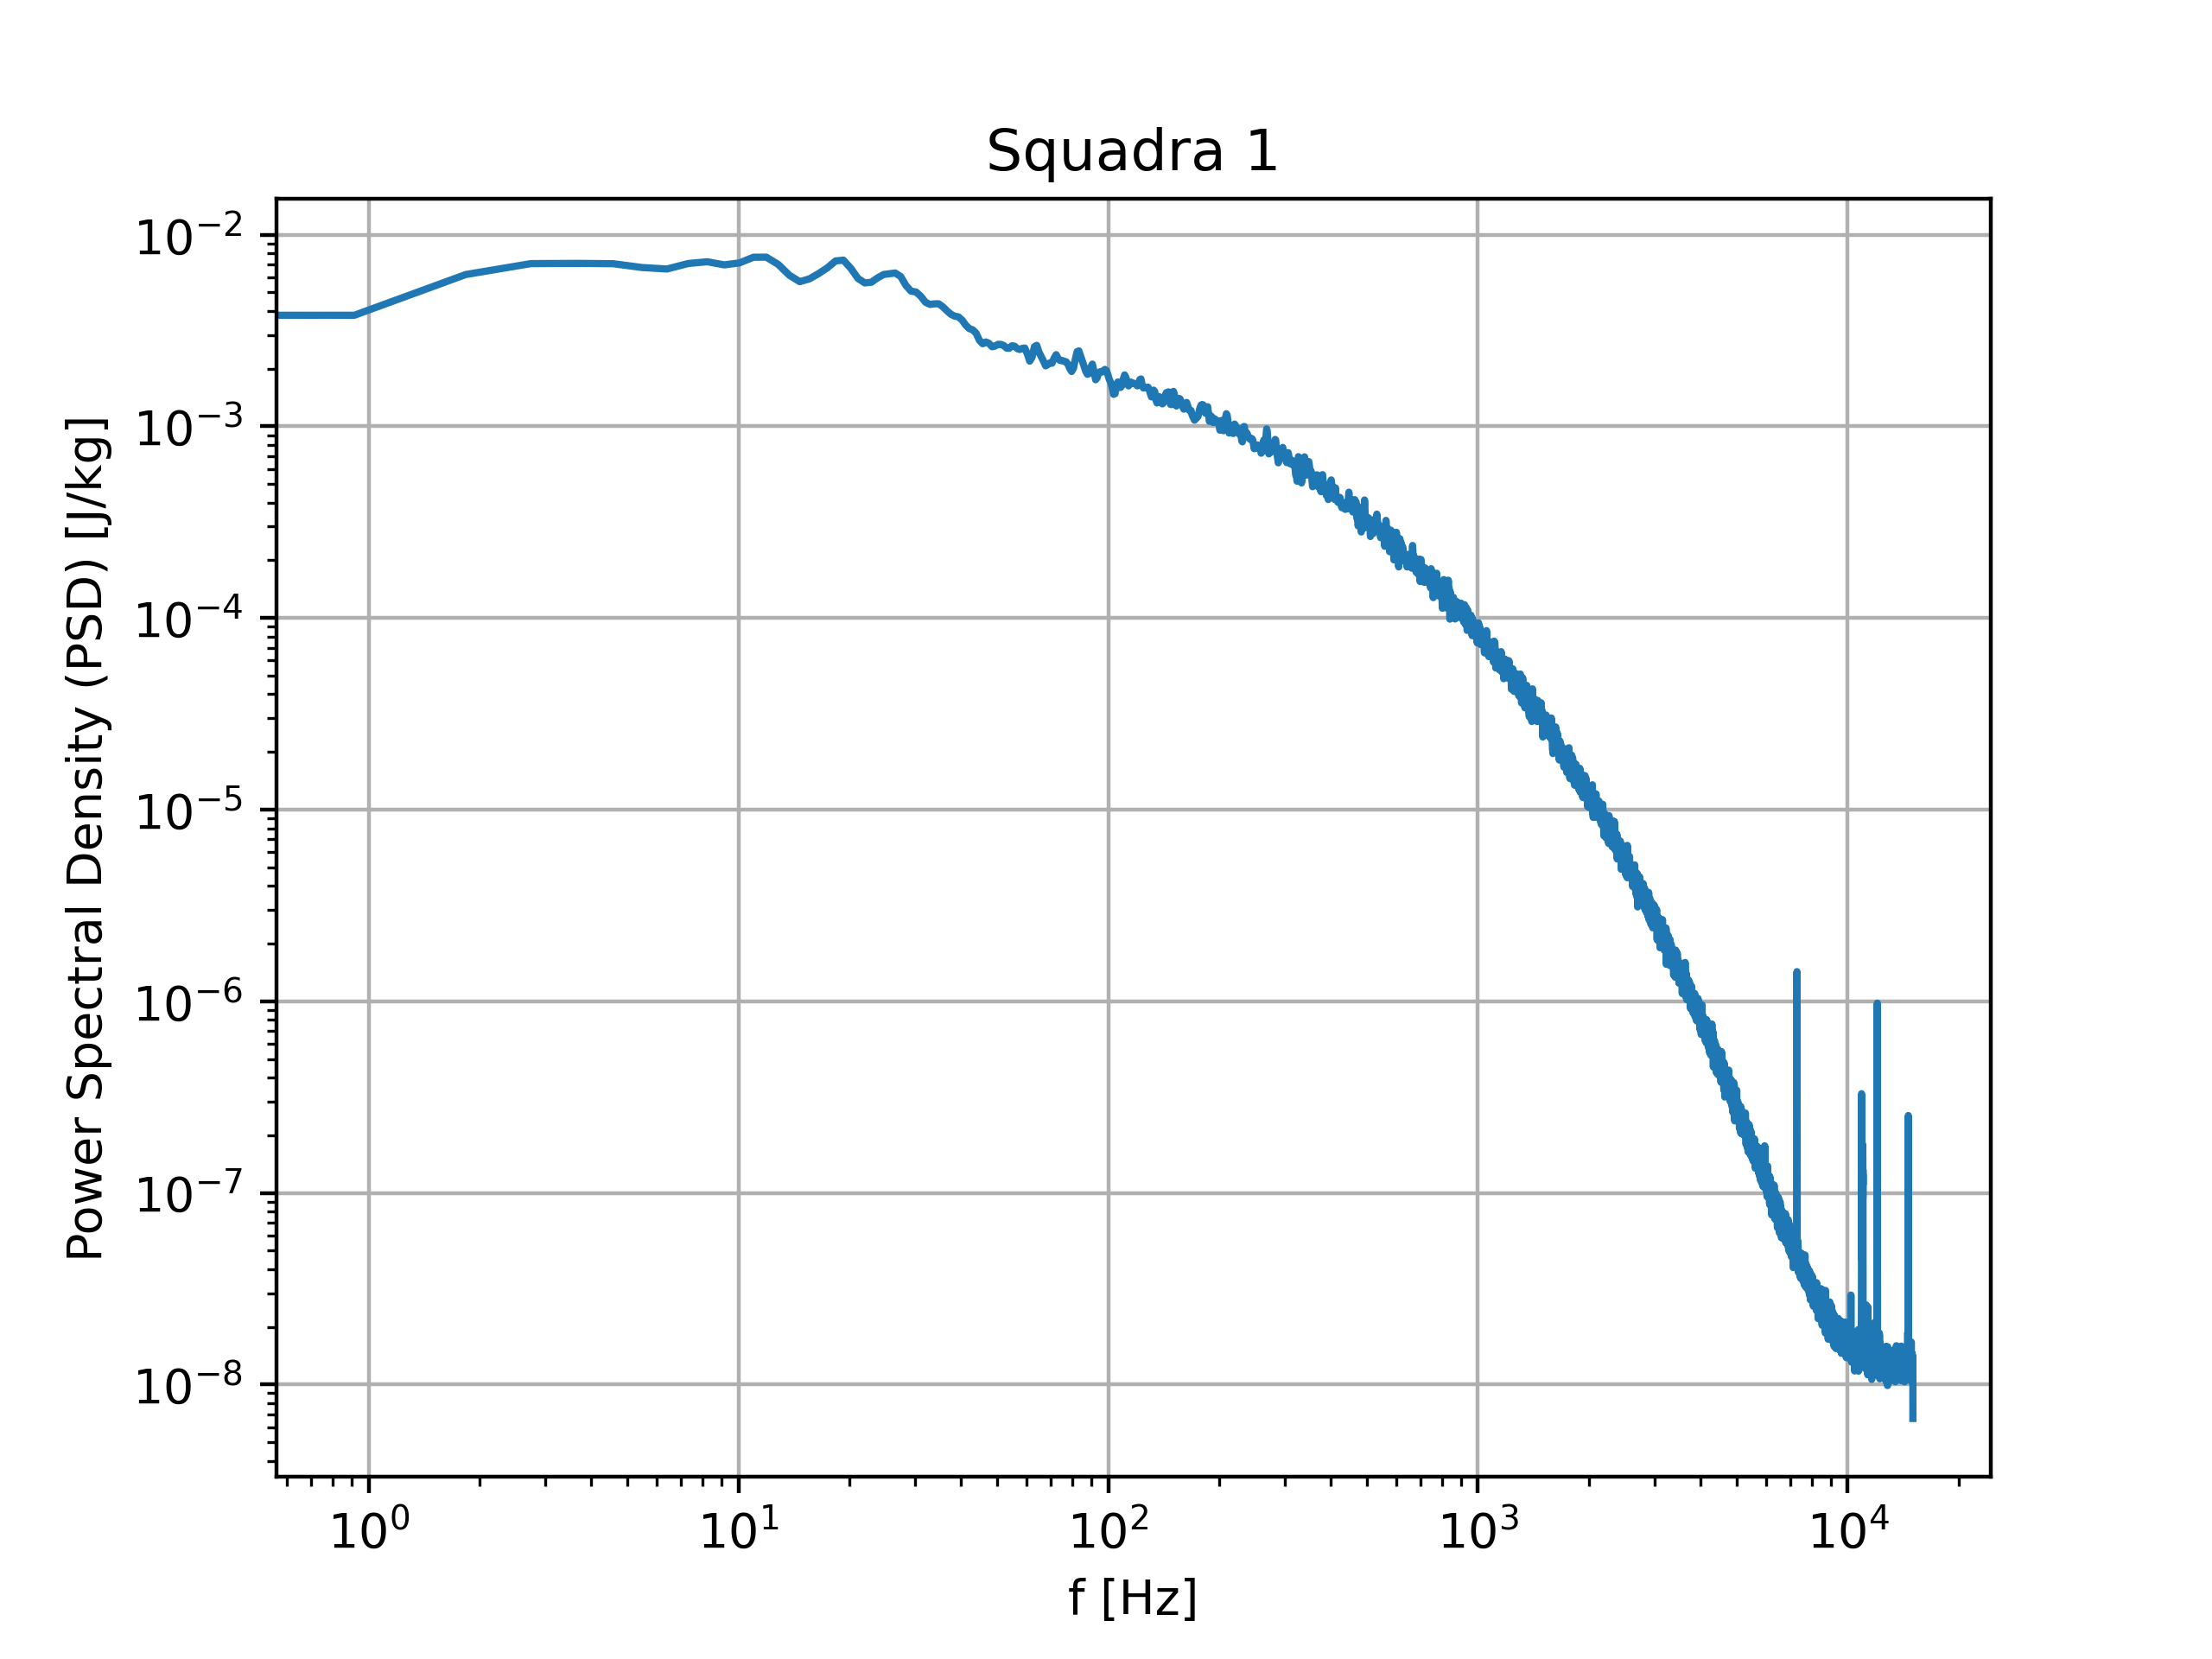
\includegraphics[width=.85\textwidth]{images/9/sq1timeserieswelchcl.png}
    \caption{Densità spettrale di potenza per la prima squadra ($L=N/100$)}
\end{figure}

\begin{figure}[H]
    \centering
    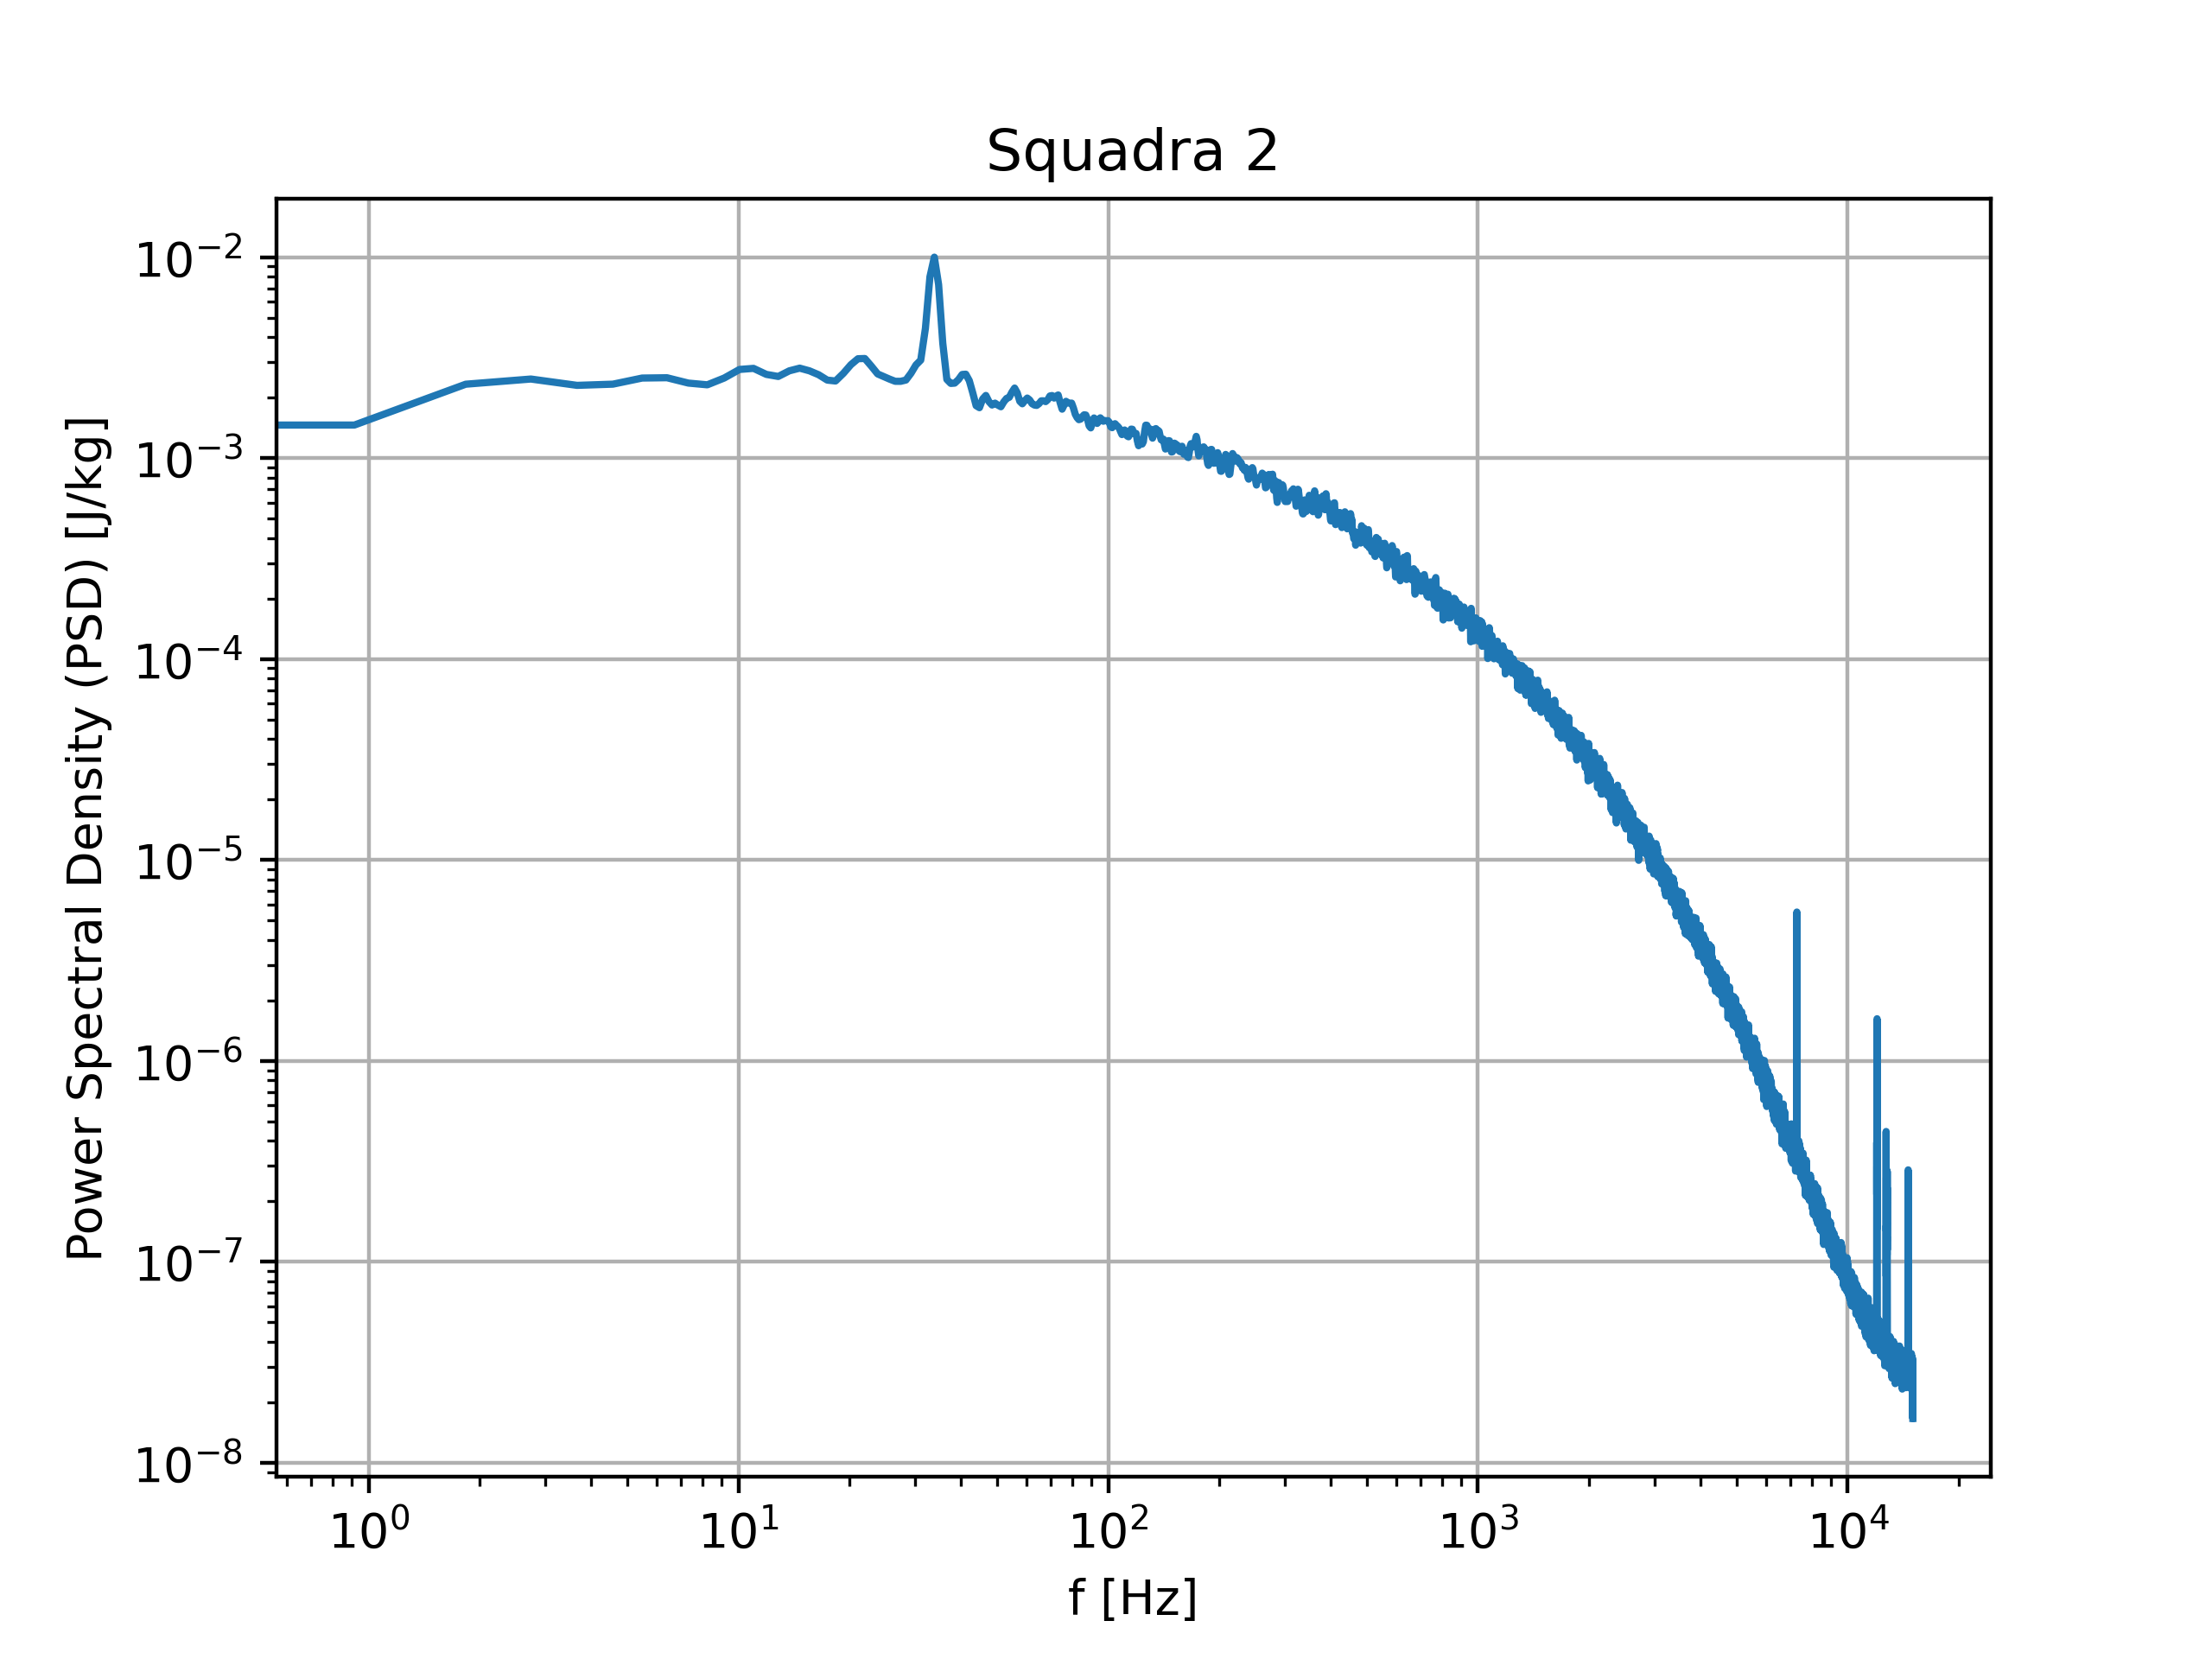
\includegraphics[width=.84\textwidth]{images/9/sq2timeserieswelchcl.png}
    \caption{Densità spettrale di potenza per la seconda squadra ($L=N/100$)}
\end{figure}

\begin{figure}[H]
    \centering
    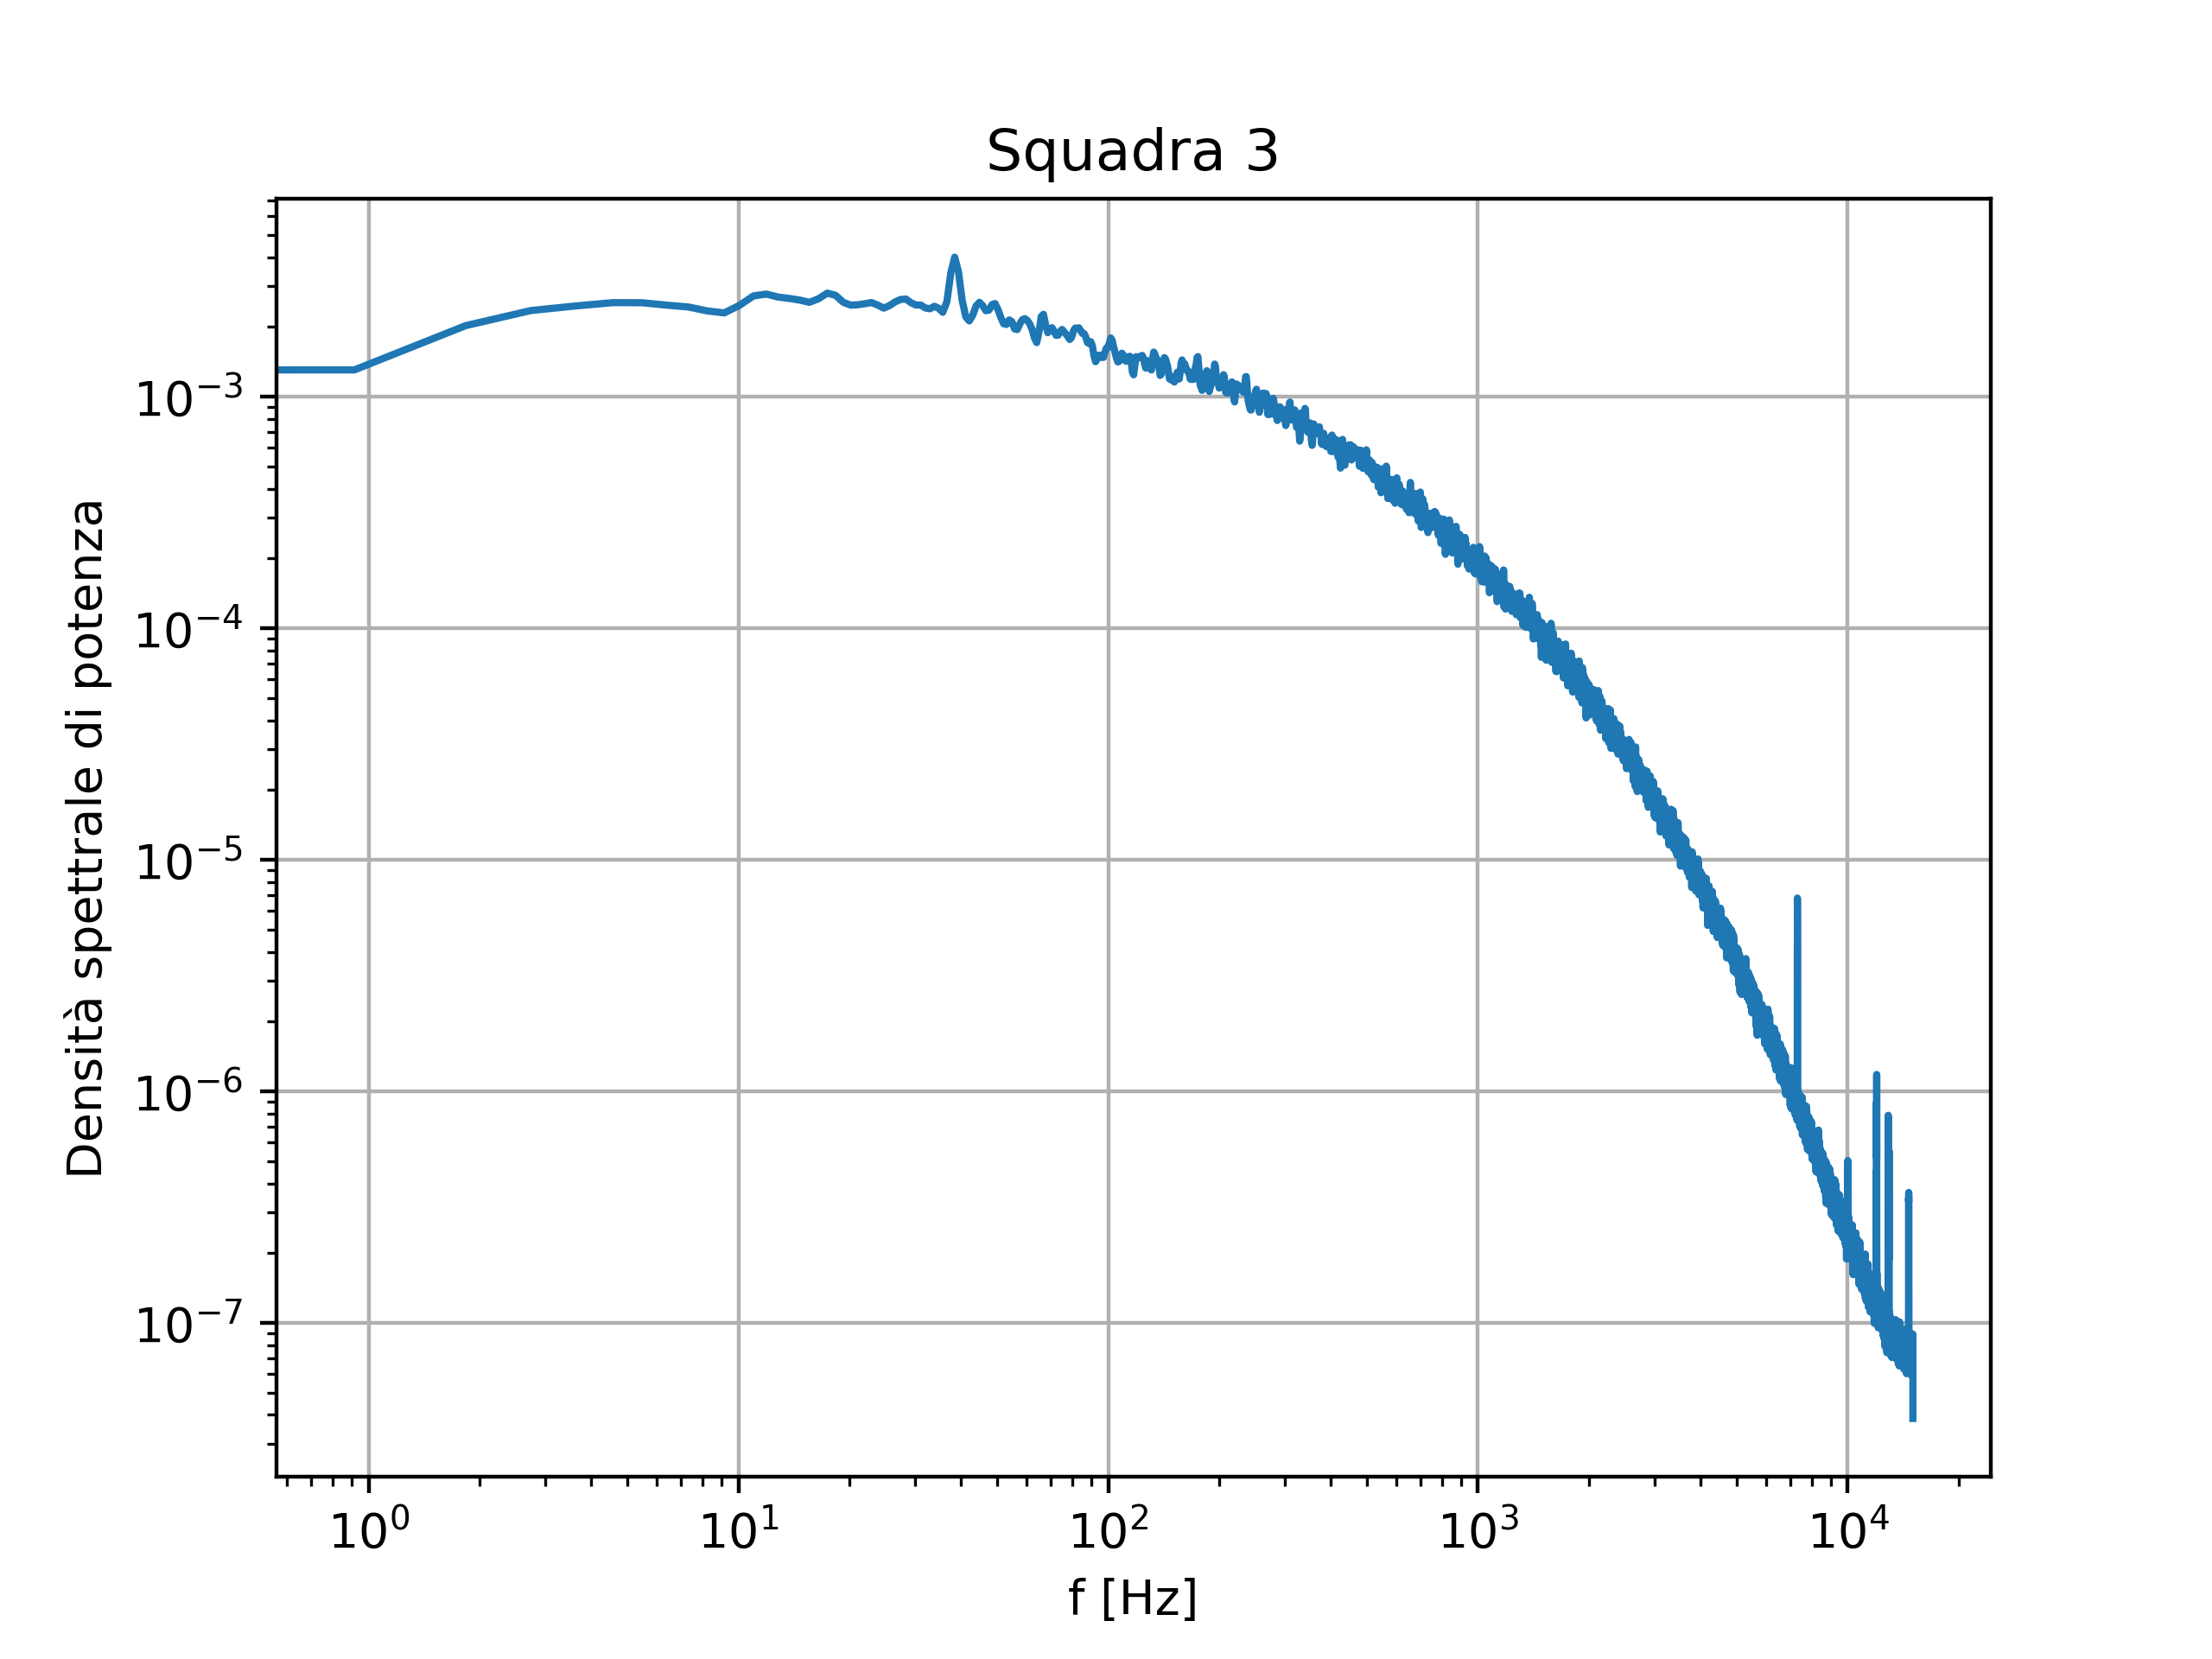
\includegraphics[width=.84\textwidth]{images/9/sq3timeserieswelchcl.png}
    \caption{Densità spettrale di potenza per la terza squadra ($L=N/100$)}
\end{figure}

\begin{figure}[H]
    \centering
    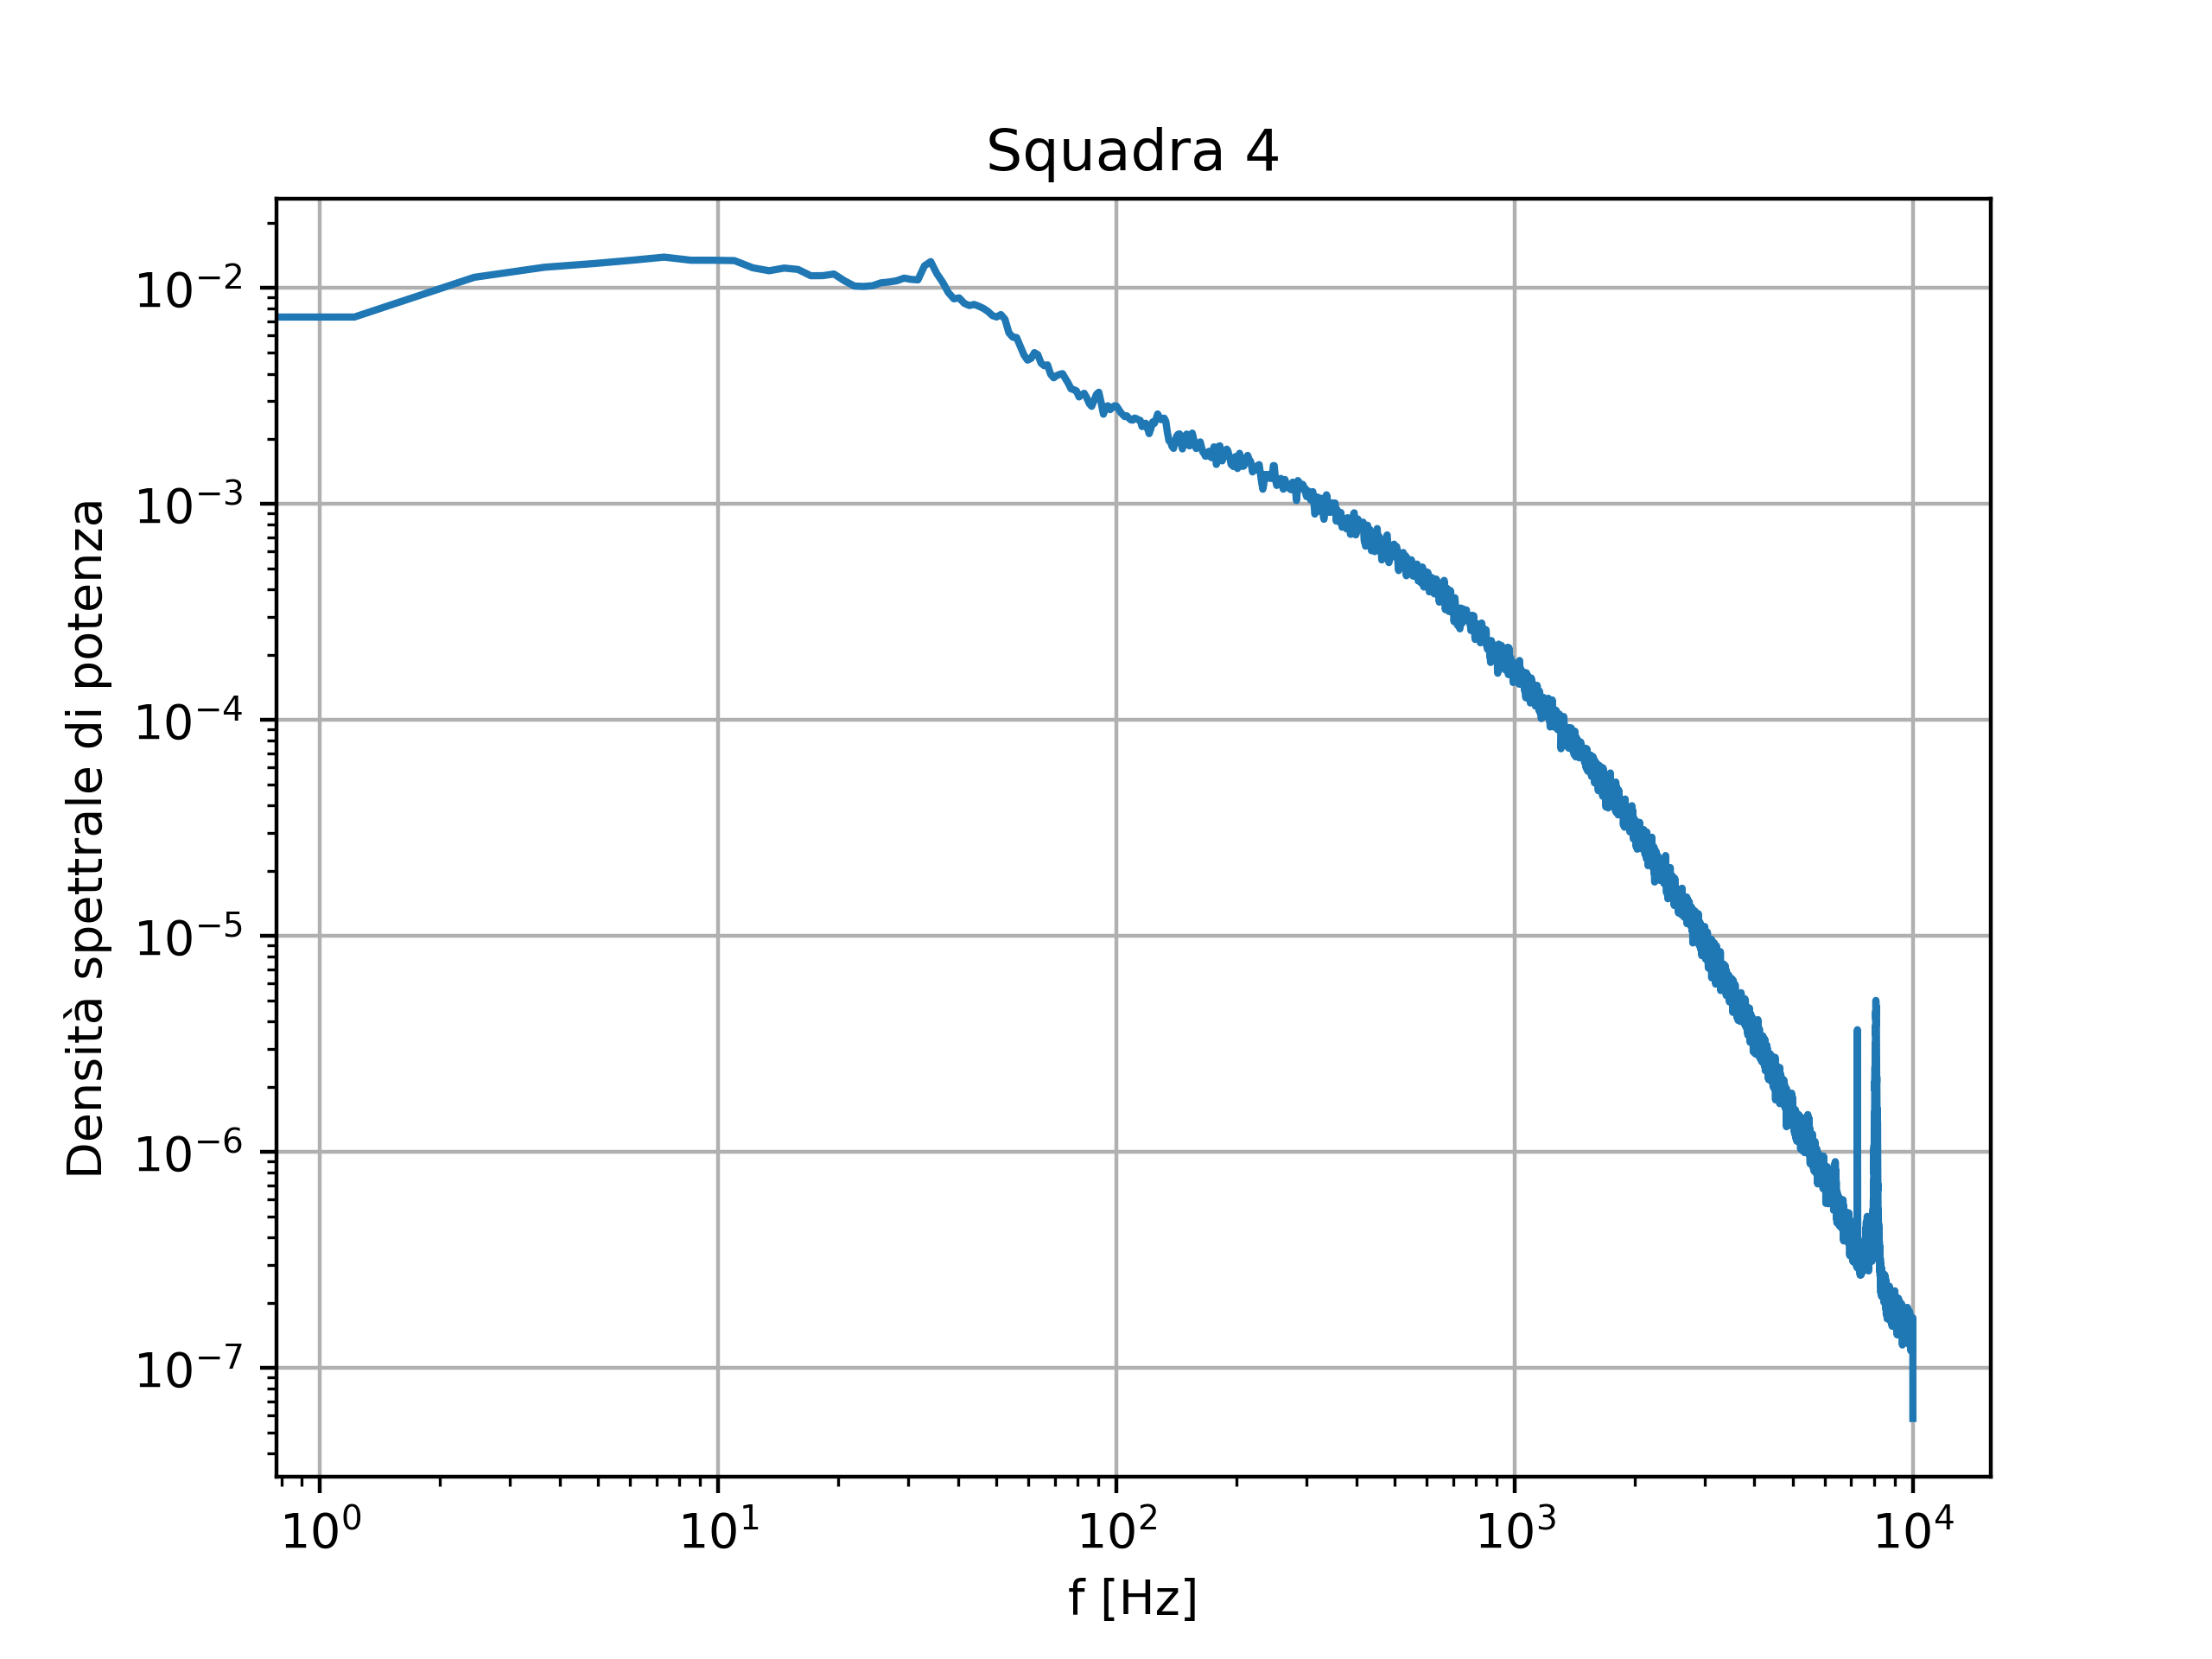
\includegraphics[width=.73\textwidth]{images/9/sq4timeserieswelchcl.png}
    \caption{Densità spettrale di potenza per la quarta squadra ($L=N/100$)}
\end{figure}

\noindent Questi diagrammi mostrano in modo molto evidente e chiaro la distribuzione energetica dello strato limite turbolento in funzione delle frequenze, tuttavia, dato il basso numero di punti per segmento, alcune frequenze caratteristiche potrebbero non essere evidenti per motivazioni di tipo numerico. Aumentando il numero di punti per segmento a $L=N/4.5$, si ottengono i seguenti diagrammi:

\begin{figure}[H]
    \centering
    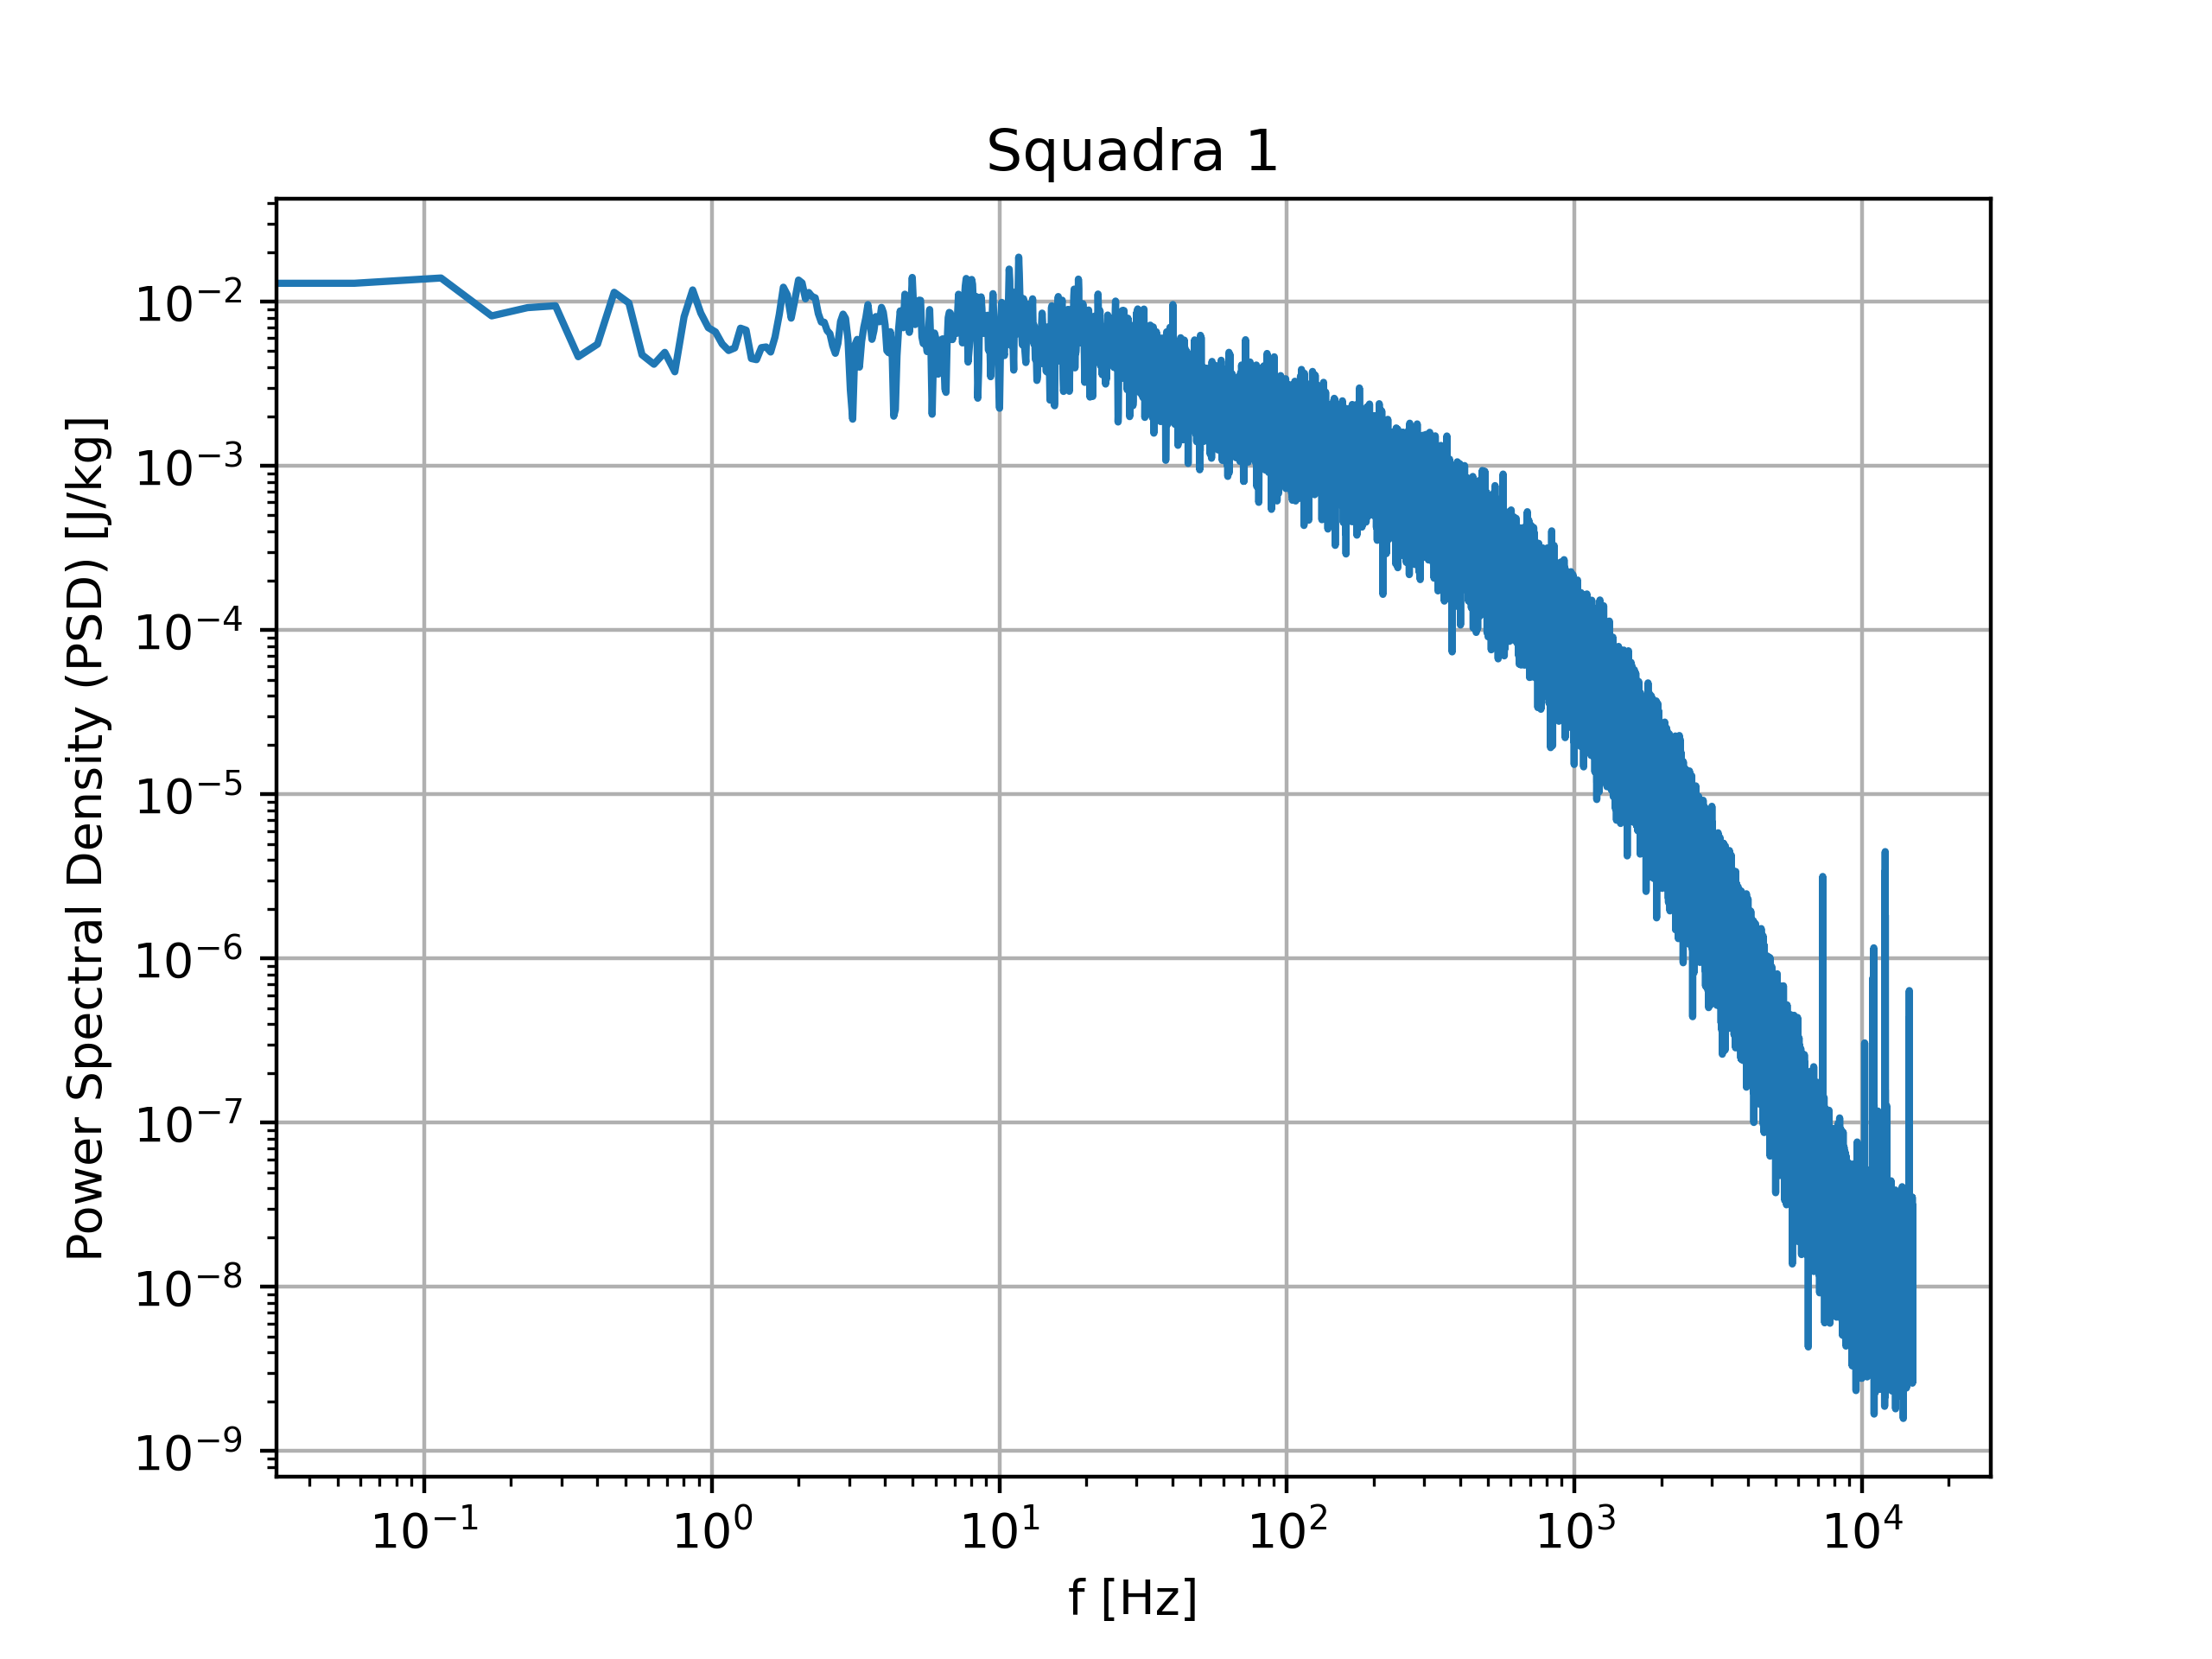
\includegraphics[width=.73\textwidth]{images/9/sq1timeserieswelch.png}
    \caption{Densità spettrale di potenza per la prima squadra ($L=N/4.5$)}
\end{figure}

\begin{figure}[H]
    \centering
    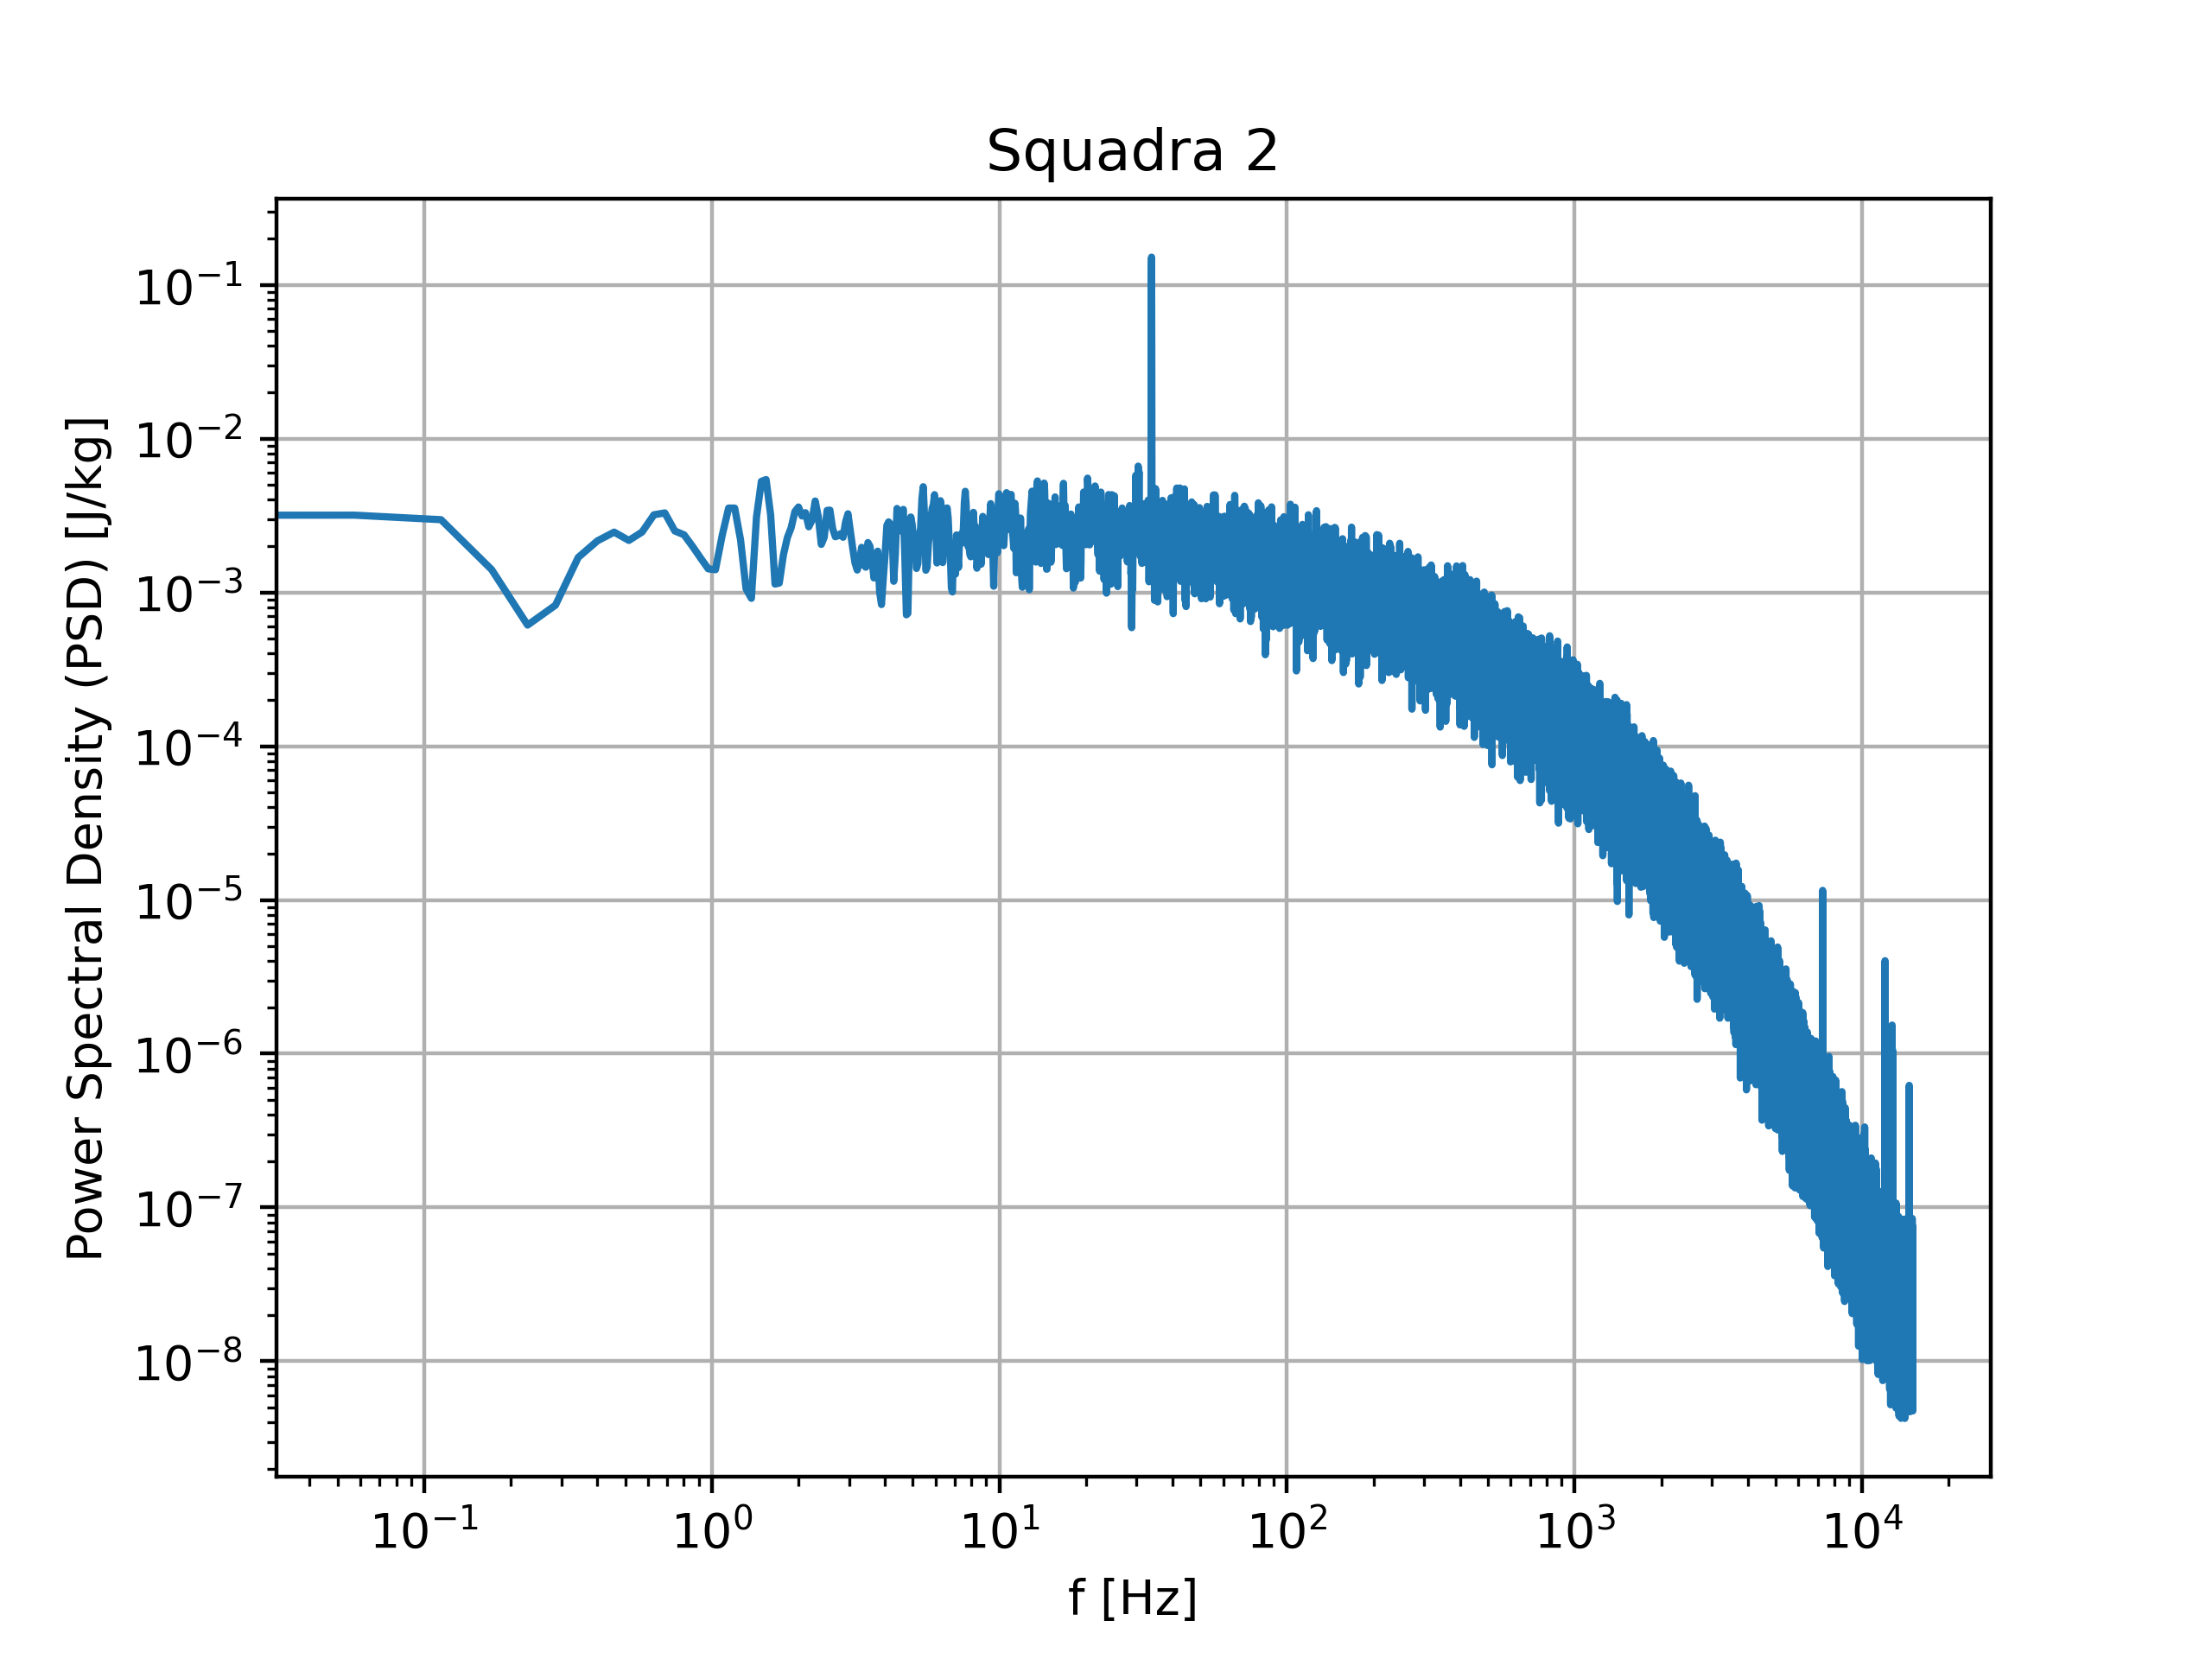
\includegraphics[width=.84\textwidth]{images/9/sq2timeserieswelch.png}
    \caption{Densità spettrale di potenza per la seconda squadra ($L=N/4.5$)}
\end{figure}

\begin{figure}[H]
    \centering
    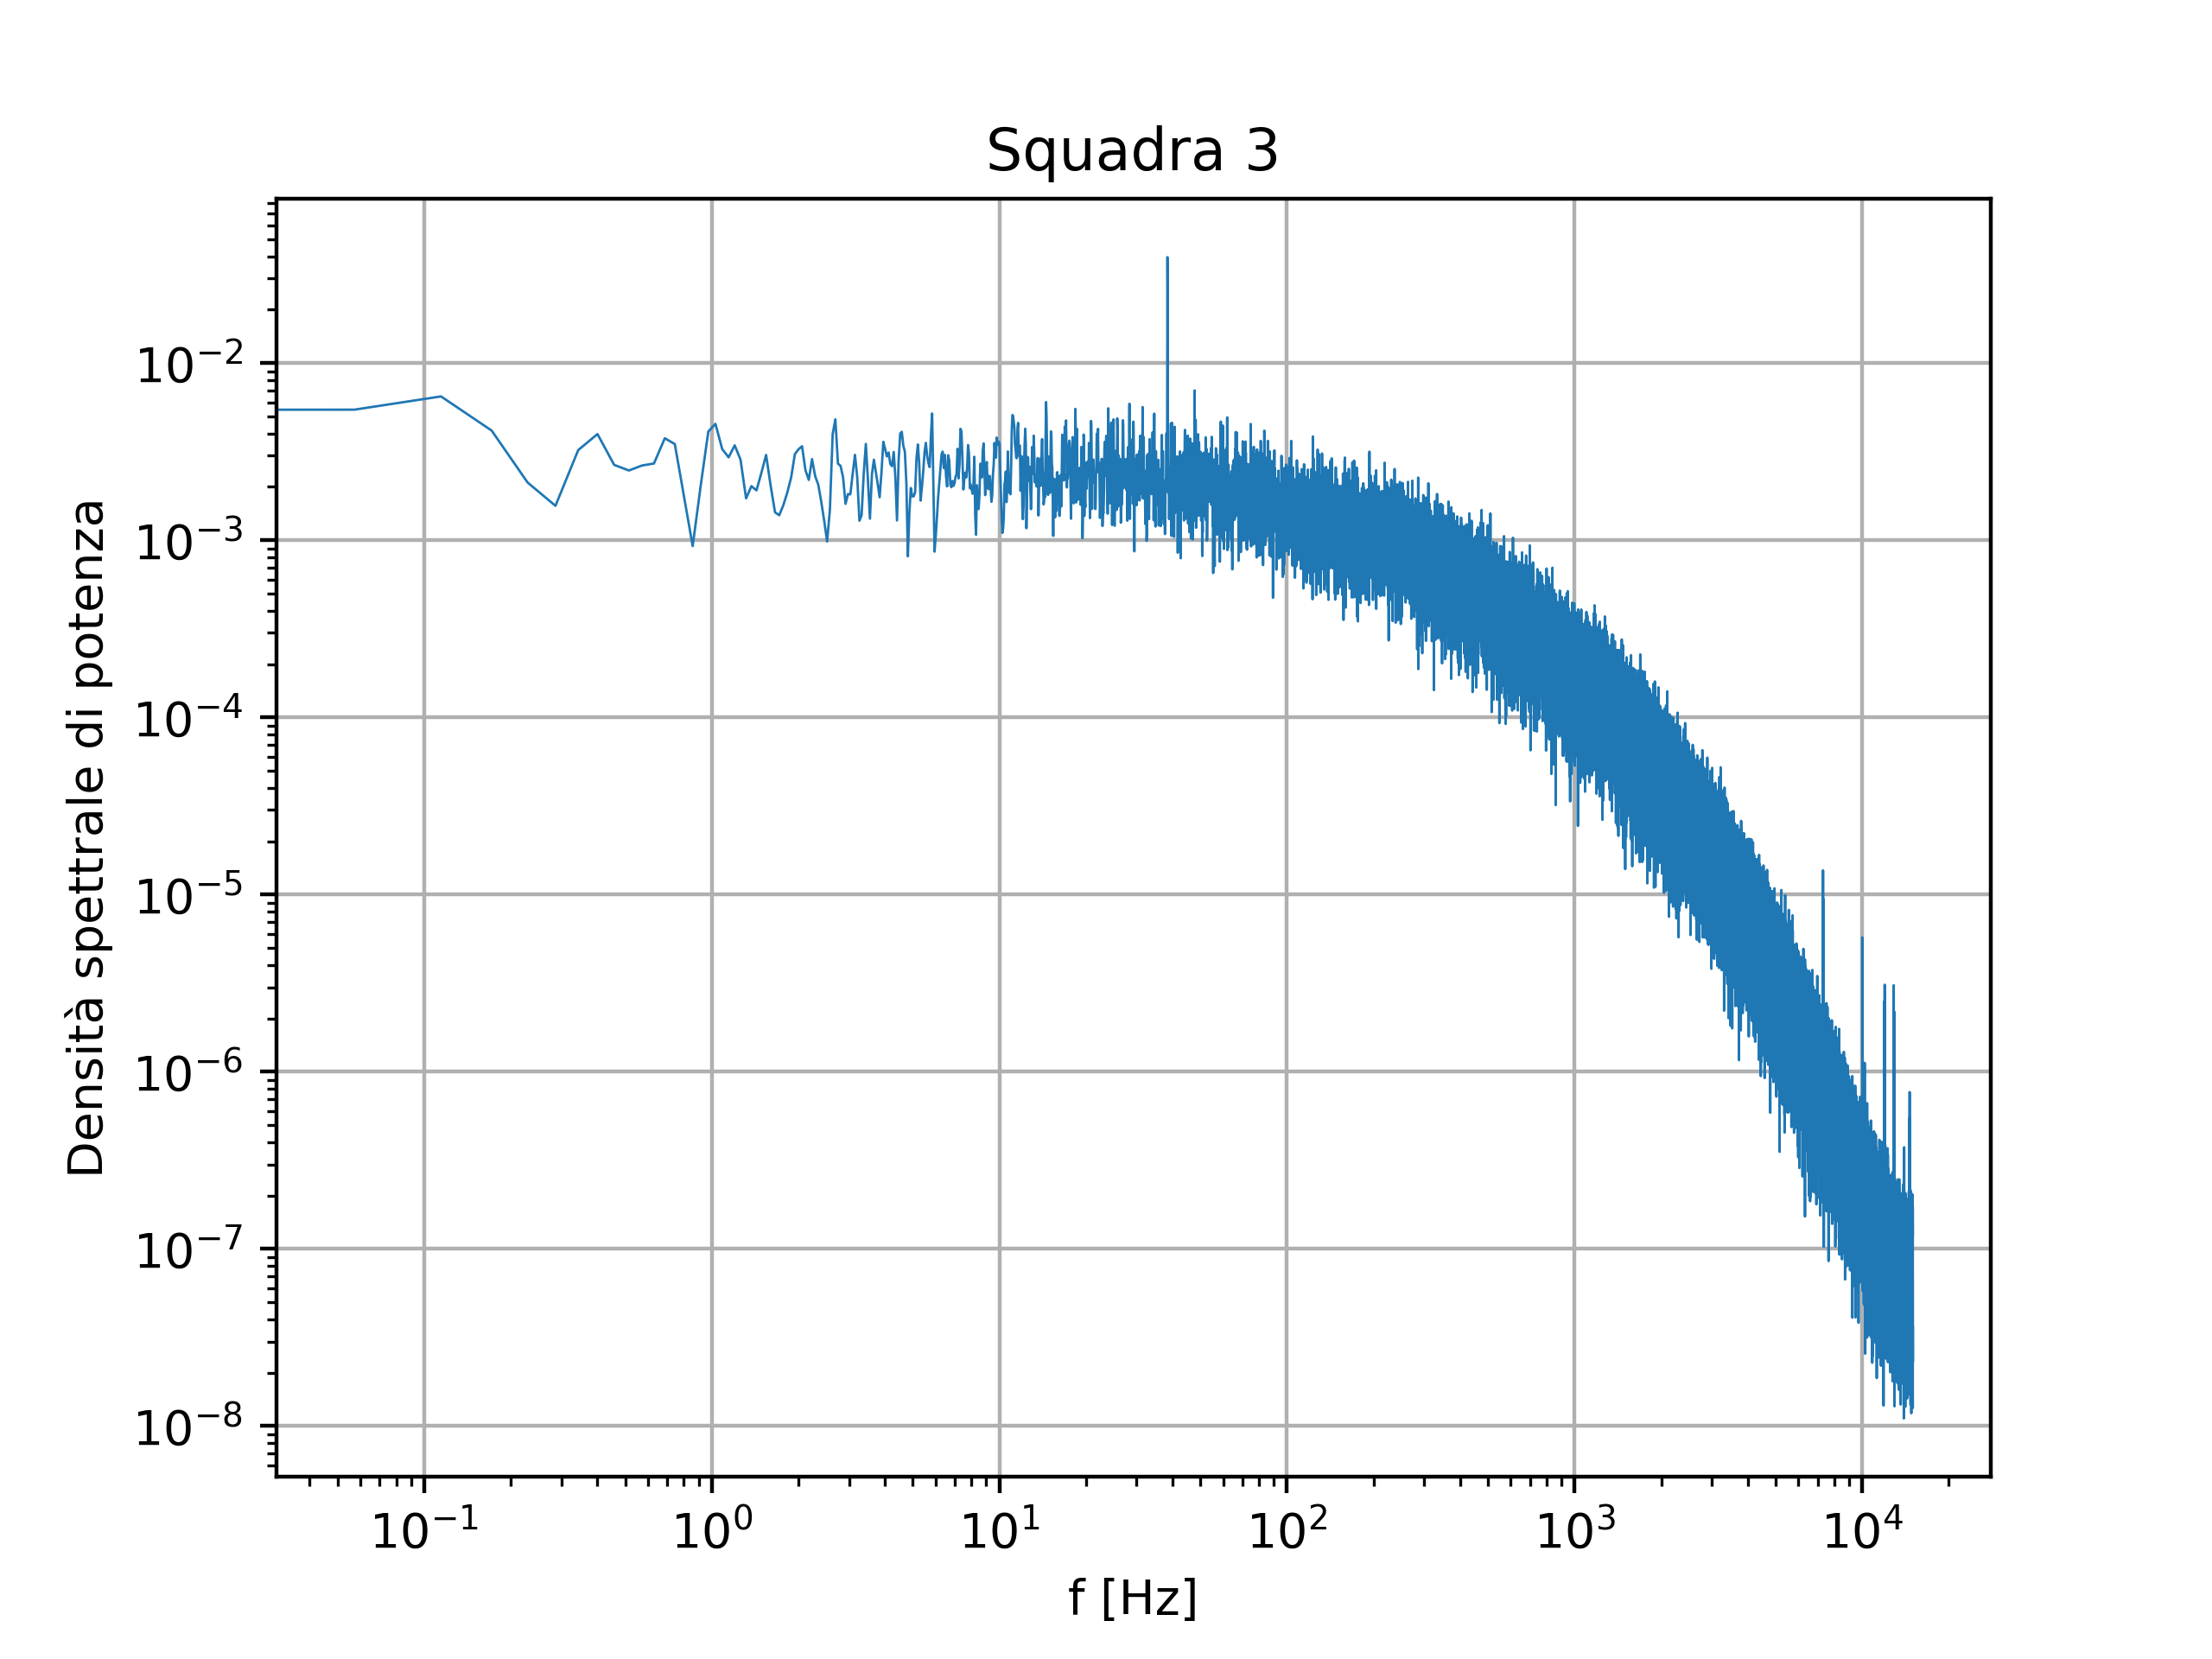
\includegraphics[width=.84\textwidth]{images/9/sq3timeserieswelch.png}
    \caption{Densità spettrale di potenza per la terza squadra ($L=N/4.5$)}
\end{figure}

\begin{figure}[H]
    \centering
    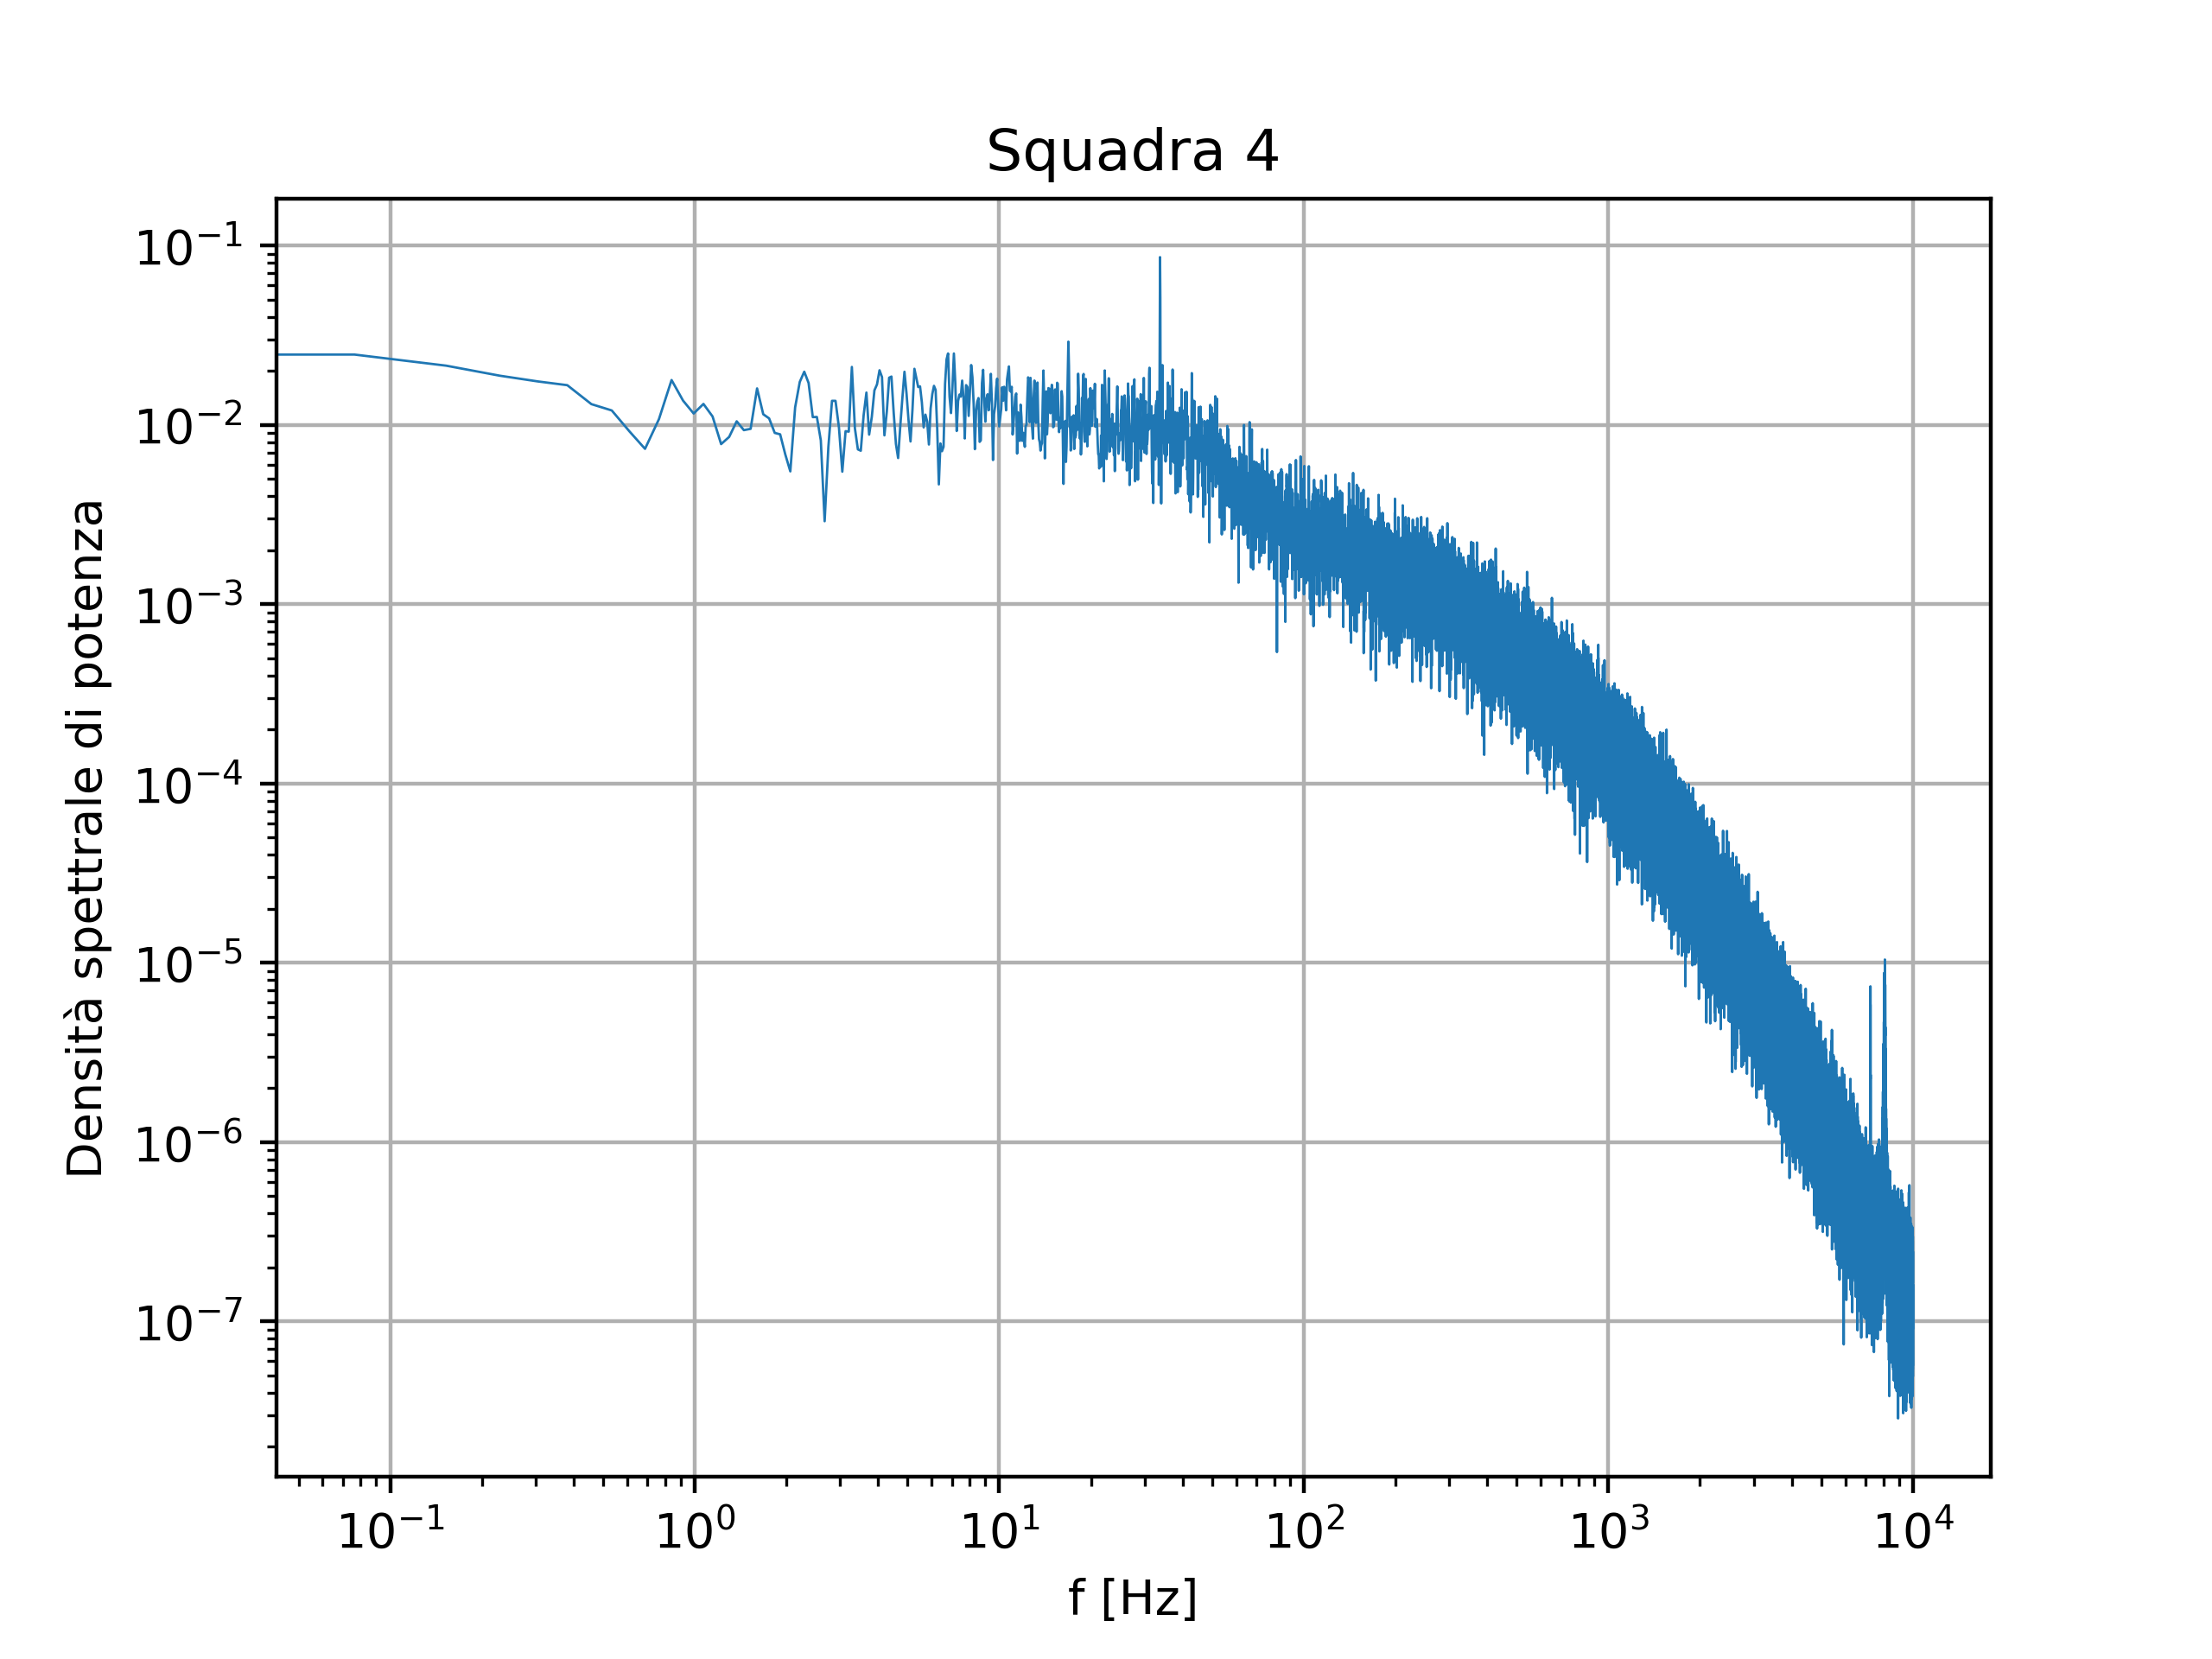
\includegraphics[width=\textwidth]{images/9/sq4timeserieswelch.png}
    \caption{Densità spettrale di potenza per la quarta squadra ($L=N/4.5$)}
\end{figure}

\noindent In questi ultimi diagrammi si evidenziano dei picchi nella densità spettrale di potenza corrispondenti a delle frequenze ($f\approx30$ Hz) caratteristiche del sistema. Questi picchi di energia possono essere dovuti a fenomeni di sfilamento vorticoso dei supporti della sonda a filo caldo o del tubo di Pitot all'ingresso della camera di prova.\\\\
I picchi di energia che invece si osservano a valori di frequenza più alti sono probabilmente dovuti a fenomeni numerici spuri o ad interferenze di tipo elettromagnetico.